% -------------------------------------------------------------------------------------
% Einlesen der .sty-Dateien
% -------------------------------------------------------------------------------------
%  se-pa1-input-styles.tex
%
%  Joerg Baumgart 01.08.2011
%
%  Zusammenfassung und Konfiguration wichtiger Styles f\"ur die 
%  Erzeugung von Seminar-, Projekt- und Bachelorarbeiten
%
%
\documentclass[12pt,BCOR=10mm,headinclude=on,footinclude=off,bibliography=totoc]{scrreprt}
\usepackage[T1]{fontenc}
\usepackage[utf8]{inputenc}
\usepackage[ngerman]{babel} % Deutsche Einstellungen
\usepackage{lmodern}

\usepackage{tikz} % Graphikpaket, das zu pdfLaTeX kompatibel ist
\usepackage{xkeyval} % Definition von Kommandos mit mehreren optionalen Argumenten
\usepackage{listings} % Formatierung von Programmlistings
\usepackage{graphicx} % Einbinden von Graphiken
\usepackage{ifthen}
\usepackage{color}
\usepackage{slashbox} % Diagonalen in Tabellenfeldern
\usepackage{framed} % Erzeugung schwarzer Linien am linken Rand zur Hervorhebung von Textteilen
\usepackage{caption} % Korrektes Setzen einer mehrzeiligen float-Unterschrift bei neu definierten float-Umgebungen
%\usepackage{floatrow}

% Es wird jeweils die sty-Datei importiert und entsprechende Konfigurationseinstellungen werden vorgenommen
%
\usepackage{sty/se-jb-scrpage2} % Formatierung der Kopf- und Fu{\ss}zeilen
\usepackage{sty/se-jb-footmisc}    % Fussnoten besser formatieren

\usepackage{sty/se-jb-glossaries} % Abk\"urzungsverzeichnis, Symbolverzeichnis, Glossar
   
\usepackage{sty/se-jb-floatrow}    % Definition und Konfiguration von float-Umgebungen (figure, table, die neue programm-Umgebung)
% Achtung: se-jb-varioref muss nach se-jb-floatrow importiert werden; 
% andernfalls ist der counter programm f\"ur die labelformat-Anweisung noch nicht definiert   
\usepackage{sty/se-jb-varioref}   % Definition von Querverweisen
\usepackage{sty/se-jb-chngcntr}   % Kapitelweise oder globale Nummerierung von Abbildungen etc.
   
\usepackage{sty/se-jb-listen} % Definition neuer, besser formatierter Listen
\usepackage{sty/se-jb-wa-kommandos} % neue Kommandos f\"ur Seminar-, Projekt- und Bachelorarbeiten


% -------------------------------------------------------------------------------------
% Individuelle Konfiguration des Dokumentes
% -------------------------------------------------------------------------------------
%  Individuelle Konfiguration einer Projektarbeit
%
%
%
%

%
% Literaturverzeichnis
% 
%\usepackage{se-jb-jurabib-theisen} % Literaturverzeichnis gem\"ass den Vorgaben von Theisen aufbauen

\usepackage{bibgerm}
\usepackage{url}
\usepackage{booktabs}
\usepackage{array}

\providecommand{\seCite}[3]{\ifthenelse{\equal{#2}{}}{#1 \cite{#3}}{#1 \cite[#2]{#3}}}


\providecommand{\seFootcite}[3]{\ifthenelse{\equal{#2}{}}{\footnote{#1 \cite{#3}}}{\footnote{#1 \cite[#2]{#3}}}}


% Weitere Optionseinstellungen f\"ur das Koma-Script
%
% Zwischen Abs\"atzen einen Abstand von 0.5 \baselineskip erzeugen
\KOMAoption{parskip}{full}
%
% Vergleiche Duden "Gliederung von Nummern, S.111" 
% DIN 5008 anschauen, wenn sie neu ver\"offentlicht wurde
\KOMAoption{numbers}{noendperiod}
%
%



%  Voreinstellungen f\"ur floats
%  Durch die verwendeten Parameter wird die Wahrscheinlichkeit deutlich kleiner, 
%  dass Gleitobjekte (z. B. Abbildungen) ans Ende des Dokumentes verschoben 
%  werden; 
%  Achtung: clearpage erzwingt die Ausgabe von Gleitobjekten
%
\renewcommand{\topfraction}{1}  % Gleitobjekte d\"urfen eine Seite zu 100% belegen 
\renewcommand{\bottomfraction}{1} % Entsprechender Wert f\"ur den unteren Teil der Seite
\renewcommand{\textfraction}{0} % Eine Seite darf auch ohne Fliesstext existieren
%%%\renewcommand{\floatpagefraction}{1} % Bedeutung unklar, daher keine Ver\"anderung des Vorgabewertes 
                                                                        % von 0.5; eventuell bringt ein \"Anderung auf 1 etwas, wenn 
                                                                         % Probleme mit floats auftreten
                                                                         
                                                                         
                                                                         
% Konfiguration von Programm-Listings
% 
% Achtung: hier gibt es nahezu beliebig viele weitere Konfigurationm\"oglichkeiten; vgl. Paketdokumentation
%
\lstset{language=[R/3 6.10]ABAP,basicstyle=\ttfamily,keywordstyle=\color{blue},captionpos=b,aboveskip=0mm,belowskip=0mm,
          xleftmargin=0em}        
          
%
% Grundkonfiguration der Abs\"ande zwischen den Items der maximal f\"unf Verschachtelungsebenen der 
% neuen Listenumgebungen
%                                                                             
% Initialisierung der Abst\"ande zwischen den items f\"ur seList; Grundeinheit: 0.5\baselineskip; siehe se-jb-listen
\seSetlistbaselineskip{1}{0.75}{0.75}{0.75}{0.75}
% Initialisierung der Abst\"ande zwischen den items f\"ur seToplist; Grundeinheit: 0.5\baselineskip; siehe se-jb-listen
\seSettoplistbaselineskip{1}{0.75}{0.75}{0.75}{0.75}     


%
%  Konfiguration der verschiedenen Verzeichnisse
%
%  abstandEintrag: Wert wird mit \baselineskip multipliziert
%

%
%  Abbildungsverzeichnis
%
\seKonfigurationAbb[
%verzeichnisname=Abbildungsverzeichnis,
labeltextLinks=, % kein Text links;
%labeltextRechts=:,
labelbreite=1cm,
%labeleinzug=1cm,
%abstandEintrag=1,
newpage=ja,
%pnumwidth=20mm,
%dotsep=1000,
%tocrmarg=4.5cm,
%abstandVerzeichnis=-1mm
]

%
% LIstingverzeichnis
%
\seKonfigurationPrg[
%verzeichnisname=Listing-Verzeichnis,
labeltextLinks=,
%labeltextRechts=:,
labelbreite=1cm,
%labeleinzug=2cm,
%abstandEintrag=1,
newpage=ja,
%%pnumwidth=20mm,
%dotsep=1000,
%tocrmarg=4.5cm,
%abstandVerzeichnis=-10mm
]

%
% Tabellenverzeichnis
%
\seKonfigurationTab[
%verzeichnisname=Liste der Tabellen,
labeltextLinks=,
%labeltextRechts=:,
labelbreite=1cm,
%labeleinzug=0.5cm,
%abstandEintrag=1,
newpage=ja,
%pnumwidth=20mm,
%dotsep=1000,
%tocrmarg=4.5cm,
%abstandVerzeichnis=-10mm
]

%
% Abk\"urzungsverzeichnis
%
\seKonfigurationAbk[
%verzeichnisname=Liste der Abk\"urzungen,
%labelbreite=3cm,
%labeleinzug=0.5cm,
%abstandEintrag=1,
%newpage=ja,
%abstandVerzeichnis=-10mm
]

%
% Symbolverzeichnis
% 
\seKonfigurationSym[
%verzeichnisname=Liste der Symbole,
%labelbreite=4cm,
%labeleinzug=3.5cm,
%abstandEintrag=1,
newpage=ja,
%abstandVerzeichnis=-10mm
]

%
% Glossar
%
\seKonfigurationGlo[
%verzeichnisname=Glossar,
%abstandEintrag=0,
]



% (eventuelle) Neudefinition f\"ur die Unter-/\"Uberschriften von Abbildungen, Tabellen und Listings
%
%
%\renewcommand{\seCaptionNameAbbildung}{Abb.}
%\renewcommand{\seCaptionNameTabelle}{Tab.}
%\renewcommand{\seCaptionNameProgramm}{Prg.}


% % (eventuelle) Neudefinition f\"ur Querverweise innerhalb des Textes
%
%
%
%\renewcommand{\seQuerverweisSeite}{Seite}
%\renewcommand{\seQuerverweisAbbildung}{Abb.}
%\renewcommand{\seQuerverweisTabelle}{Tab.}
%\renewcommand{\seQuerverweisProgramm}{Prg.}
%\renewcommand{\seQuerverweisKapitel}{Kap.}
%\renewcommand{\seQuerverweisGleichung}{Gl.}

% Kommandos, die direkt nach \begin{document} ausgef\"uhrt werden m\"ussen
%
%
%
\AtBeginDocument{%
\renewcommand{\listfigurename}{\seAbbildungenVerzeichnisname}
\renewcommand{\listtablename}{\seTabellenVerzeichnisname}
\renewcommand{\figurename}{\seCaptionNameAbbildung}
\renewcommand{\tablename}{\seCaptionNameTabelle}
\pagenumbering{roman}
}
                                                              
                                                                         

% -------------------------------------------------------------------------------------
% Individuelle Definition von Abk\"urzungen, Symbolen und eventuell Glossareintr\"agen
% -------------------------------------------------------------------------------------
%--------------------------------------------------------------------------------------
% Trennungsregeln
%--------------------------------------------------------------------------------------
\hyphenation{prob-lem-los}
\hyphenation{Inter-banken-han-del}
\hyphenation{Business-Objects}
\hyphenation{Web-ser-vice}
\hyphenation{Web-ser-vi-ces}
\hyphenation{Dash-board}
\hyphenation{Dash-boards}
\hyphenation{Zu-gangs-be-schrän-kung-en}
\hyphenation{ge-star-tet}
\hyphenation{NSFR}
\hyphenation{LCR}
\hyphenation{Va-ri-a-blen-aus-prä-gung-en}
\hyphenation{Dia-gramm}
\hyphenation{An-wen-dung}
\hyphenation{An-wen-dung-en}
\hyphenation{An-for-de-rung}
\hyphenation{An-for-de-rung-en}
\hyphenation{Haupt-an-for-de-rung-en}
\hyphenation{tech-nisch-en}
\hyphenation{Funk-ti-o-na-li-tät}
\hyphenation{Or-ches-trie-rung}
\hyphenation{Xcel-si-us}
\hyphenation{Xcel-si-us-A-dap-ter}
\hyphenation{Ein-stel-lung}
\hyphenation{Ein-stel-lung-en}
\hyphenation{Li-qui-di-tät}
\hyphenation{Li-qui-di-täts-ri-si-ko}
\hyphenation{Li-qui-di-täts-ri-si-ko-ma-nage-ment}
\hyphenation{Dash-board}


%--------------------------------------------------------------------------------------
% Abkürzungen
%--------------------------------------------------------------------------------------
\newacronym{dbms}{DBMS}{Da\-ten\-bank\-ma\-nage\-ment\-sys\-tem}
\newacronym{sql}{SQL}{Structured Query Language}
\newacronym{MaRisk}{MaRisk}{Mindestanforderungen an das Risikomanagement}
\newacronym{LiqV}{LiqV}{Liquiditätsverordnung}
\newacronym{ngap}{NGAP}{Next Generation ABAP Plattform}
\newacronym{erp}{ERP}{Enterprise Resource Planning}
\newacronym{crm}{CRM}{Customer Relationship Management}
\newacronym{saplrm}{SAP\,\,LRM}{SAP Liquidity Risk Management}
\newacronym{http}{HTTP}{Hypertext Transfer Protocol}
\newacronym{xml}{XML}{Extensible Markup Language}
\newacronym{NetWeaver}{NetWeaver}{SAP NetWeaver Application Server}
\newacronym{xcelsius}{Xcelsius}{BusinessObjects Xcelsius}
\newacronym{biz}{BIZ}{Bank für Internationalen Zahlungsausgleich}
\newacronym{url}{URL}{Uniform Resource Locator}
\newacronym{wysiwyg}{WYSIWYG}{What You See Is What You Get}
\newacronym{sdk}{SDK}{Software Development Kit}
\newacronym{lcr}{LCR}{Liquidity Coverage Ratio}
\newacronym{nsfr}{NSFR}{Net Stable Funding Ratio}
\newacronym{rest}{REST}{Representational State Transfer}
\newacronym{ria}{RIA}{Rich Internet Application}
\newacronym{abap}{ABAP}{Advanced Business Application Programming}
\newacronym{bw}{BW}{Business Warehouse}
\newacronym{libor}{LIBOR}{London Inter Bank Offered Rate}

%--------------------------------------------------------------------------------------
% Glossareinträge
%--------------------------------------------------------------------------------------

\newglossaryentry{glos:netFramework}{
first=.NET Framework\textsuperscript{GL},
name=.NET Framework,
description={ Das .NET Framework ist eine Plattform von Microsoft, mit der Anwendungen für das Betriebssystem Microsoft Windows erstellt und ausgeführt werden können. Die wichtigsten Komponenten sind Klassenbibliotheken, zum Beispiel für die Entwicklung der Oberflächen, und die Common Language Runtime. Die Anwendungen können in verschiedenen Programmiersprachen geschrieben werden. Zu den unterstützten Sprachen zählen unter anderem C++ und C\#. Der Quellcode wird dann in die Common Intermediate Language compiliert. Diese Zwischensprache kann dann von der Common Language Runtime ausgeführt werden.\seFootcite{vgl.}{S.382ff}{Lou.10}}
}


\newglossaryentry{glos:interbankenhandel}{
first=Inter\-banken\-han\-del\textsuperscript{GL},
name=Interbankenhandel,
description={Der Interbankenhandel ist der Handel von Wertpapieren, Anlagen oder ähnlichem zwischen Banken. Synonym wird auch oft der Begriff Interbankenmarkt verwendet. Für die Zinssätze, mit denen Banken untereinander handeln, existieren anerkannte Referenzen, wie zum Beispiel die \gls{libor}. In Liquiditätsengpässen kann der Interbankenhandel eine wichtige Refinanzierungsrolle darstellen. Der Handel zwischen Banken hängt sehr stark von dem gegenseitigen Vertrauen ab.\seFootcite{vgl.}{S.145f}{Wil.10}}
}

\newglossaryentry{glos:bankrun}{
first=Bankenpanik\textsuperscript{GL},
name=Bankenpanik,
description={Eine Bankenpanik ist ein Ereignis, bei dem eine große Anzahl von Anlegern versucht, ihre Einlagen bei einer Bank abzuziehen. Der Grund kann zum einen in der Veröffentlichung von schlechten Ergebnissen der Bank und damit in einem Vertrauensverlust begründet sein, zum anderen aber auch rein spekulativ sein. Für die Bank besteht die Gefahr der Insolvenz. Im Englischen spricht man von einem Bank Run.\seFootcite{vgl.}{S.1f}{Sch.11}}
}

\newglossaryentry{glos:sqlscript}{
first=SQLScript\textsuperscript{GL},
name=SQLScript,
description={SQLScript ist eine Erweiterung der Abfragesprache SQL und wird in der Datenbank von SAP HANA verwendet. Mit Hilfe von SQLScript lässt sich Anwendungslogik in die Datenbank auslagern. Dazu wurden unter anderem Datentypen, Prozeduren und Kontrollstrukturen hinzugefügt.\seFootcite{vgl.}{S.9f}{SQLScript.11}}
}

\newglossaryentry{glos:ria}{
first=\gls{ria}\textsuperscript{GL},
name=\gls{ria},
sort=RIA,
description={Unter dem Begriff Rich Internet Application werden Webanwendungen bezeichnet, die in ihrer Funktionalität und ihrem Aussehen Desktopanwendungen ähneln. Erstmals eingeführt wurde der Begriff von Macromedia. Zwischen normalen Webanwendungen und RIA kann keine klare Grenze gezogen werden. Ein wichtiges Indiz für eine RIA ist der Einsatz von Technologien wie zum Beispiel Adobe Flash, Adobe Air oder Microsoft Silverlight.\footnote{\seCite{vgl.}{S.32f}{DD.08} \seCite{und}{S.3f}{Pfe.09}\newline
Adobe Flash - http://www.adobe.com/products/flashplayer.html \newline
Adobe Air - http://www.adobe.com/products/air.html \newline
Microsoft Silverlight - http://www.microsoft.com/silverlight/} }
}

\newglossaryentry{glos:bydesign}{
first=SAP Business ByDesign\textsuperscript{GL},
name=SAP Business ByDesign,
description={SAP Business ByDesign ist eine Anwendung von SAP für mittelständige Unternehmen. Zu dem Funktionsunfang gehört sowohl ein \gls{erp}- als auch eine \gls{crm}-Lösung. Die Besonderheit von SAP Business ByDesign ist, dass es auf Servern bei SAP betrieben wird und Kunden die Anwendung mieten und über das Internet konsumieren.}
}

\newglossaryentry{glos:lcr}{
first=\gls{lcr}\textsuperscript{GL},
name=\gls{lcr},
sort=LCR,
description={
Die \gls{lcr}, die auch als Mindestliquiditätsquote bezeichnet wird, ist eine requlatorische Vorgabe im Rahmen von Basel III. Durch die Einhaltung soll sichergestellt werden, dass eine Bank unerwartete Zahlungsmittelabflüsse über einen Zeitraum von 30 Tagen mit eigenen liquiden Aktiva ausgleichen kann.\seFootcite{vgl.}{S.4}{BIS.10}
}
}

\newglossaryentry{glos:nsfr}{
first=\gls{nsfr}\textsuperscript{GL},
name=\gls{nsfr},
sort=NSFR,
description={
Die \gls{nsfr} ist eine requlatorische Vorgabe im Rahmen von Basel III und soll eine mittel- und langfristige Refinanzierung von Banken fördern. Er besteht aus dem Verhältnis von verfügbaren und erforderlichen langfristiger Refinanzierung. Sie wird auch als strukturelle Liquiditätsquote beizeichnet.\seFootcite{vgl.}{S.28}{BIS.10}
}
}

\newglossaryentry{glos:sdk}{
first=\gls{sdk}\textsuperscript{GL},
name=\gls{sdk},
sort=SDK,
description={
Ein \gls{sdk} besteht aus einer Reihe von Anwendungen, mit deren Hilfe Anwendungen erstellt werden können. Meistens gehört zum Umfang eines \gls{sdk} auch eine Dokumentation der Programmierschnittstelle und eine Entwicklungsumgebung dazu.
}
}

\newglossaryentry{glos:atom}{
first=Atom Syndication Format\textsuperscript{GL},
name=Atom Syndication Format,
description={
Das Atom Syndication Format ist ein XML-basierendes Format für den plattformunabhängigen Austausch von Informationen. Es wird in der Regel für sich periodisch änderne Informationen, wie zum Beispiel Newsfeeds, genutzt.\seFootcite{vgl.}{}{ATOM.07}
}
}

\newglossaryentry{glos:tomcat}{
first=Apache Tomcat\textsuperscript{GL},
name=Apache Tomcat,
description={
Der Apache Tomcat ist ein Projekt der Apache Software Foundation, mit dem Java-Code auf Webservern ausgeführt werden kann. Dadurch können dynamische Webanwendungen entwickelt werden.
}
}

\newglossaryentry{glos:rest}{
first=\gls{rest}\textsuperscript{GL},
name=\gls{rest},
sort=REST,
description={
\gls{rest} ist ein Paradigma für die Umsetzung von Webservices. Dabei sieht es vor, dass eine Ressource eindeutig über einen Uniform Resource Identifier identifiziert werden kann. Diese Ressource kann in verschiedenen Repräsentationen abgerufen werden. Auf Ressourcen lassen sich festgelegte Operationen anwenden. Die Kommunikation findet immer zustandslos statt.\seFootcite{vgl.}{S.245f}{RRD.07}
}
}

\newglossaryentry{glos:actionscript}{
first=ActionScript\textsuperscript{GL},
name=ActionScript,
description={
ActionScript ist die Programmiersprache für die Entwicklung von Adobe Flex-basierenden Programmen. ActionScript unterstützt die objektorientierte Programmierung und basiert auf dem Sprachkern von JavaScript. Für die Entwicklung existiert mit dem Flex Builder eine integrierte Entwicklungsumgebung.\seFootcite{vgl.}{S.3f}{Moo.07}
}
}


\newglossaryentry{glo:abap}{
first=\gls{abap}\textsuperscript{GL},
name=\gls{abap},
sort=ABAP,
description={
\gls{abap} ist eine Programmiersprache der vierten Generation. Sie wird für einen Großteil der von SAP entwickelten Anwendungen verwendet. Eine Besonderheit von \gls{abap} ist die einfache Integration von \gls{sql}-Abfragen. Mit \gls{abap} Objects ist auch die objektorientierte Programmierung möglich.
}
}

%TODO Generell keine Fußnoten nutzen, sondern lieber Glossar oder im Text!

\usepackage{setspace} 
\usepackage{enumitem} 

\usepackage{todonotes}

\newcounter{todocounter}
\newcommand{\todonum}[2][]
{\stepcounter{todocounter}\todo[#1]{\thetodocounter: #2}}

% -------------------------------------------------------------------------------------
% Anforderugnen
% -------------------------------------------------------------------------------------

\newcounter{anforderung}

\newcommand{\class}[1]{\textit{#1}}

\newcommand{\instance}[1]{\textit{#1}}

\newcommand{\method}[1]{\textit{#1}}

\newcommand{\anfl}[1]{
	\refstepcounter{anforderung}
	(A\arabic{anforderung})
	\label{anf:#1}
}

\newcommand{\anfRef}[2]{\ifthenelse {\equal{\pageref{#1}}{\thepage}}    {Anforderung \ref{#1} #2(A\ref{#1})}{Anforderung \ref{#1} #2(A\ref{#1} auf \pageref{#1})}}


\newcommand{\usecaseRef}[1]{\ifthenelse {\equal{\pageref{#1}}{\thepage}}{}{ auf \pageref{#1}}}

\newcommand{\useCaseItem}[2]{
\item[~~\textbf{#1}] #2
}


\newcommand{\loreIpsum}{Lorem ipsum dolor sit amet, consetetur sadipscing elitr, sed diam nonumy eirmod tempor invidunt ut labore et dolore magna aliquyam erat, sed diam voluptua. At vero eos et accusam et justo duo dolores et ea rebum. Stet clita kasd gubergren, no sea takimata sanctus est Lorem ipsum dolor sit amet. Lorem ipsum dolor sit amet, consetetur sadipscing elitr, sed diam nonumy eirmod tempor invidunt ut labore et dolore magna aliquyam erat, sed diam voluptua. At vero eos et accusam et justo duo dolores et ea rebum. Stet clita kasd gubergren, no sea takimata sanctus est Lorem ipsum dolor sit amet. Lorem ipsum dolor sit amet, consetetur sadipscing elitr, sed diam nonumy eirmod tempor invidunt ut labore et dolore magna aliquyam erat, sed diam voluptua.\todonum{Text Schreiben [HIGH]}}

\newcommand{\useCaseEntry}[2]{
\textbf{#1} 
\vspace*{-4mm}
\begin{addmargin}[3mm]{0cm} #2
\end{addmargin} 
}

\newcommand{\useCase}[2]{
\begin{mdframed}
{\large \textbf{Anwendungsfall #1}}
#2
\end{mdframed}

}

% Abstand vor Chapter überschriften
\renewcommand*{\chapterheadstartvskip}{\vspace*{-\topskip}}

\addtocontents{toc}{\vspace{-3ex}}



\renewcommand{\textfraction}{0.05}
\renewcommand{\topfraction}{0.95}
\renewcommand{\bottomfraction}{0.95}
\renewcommand{\floatpagefraction}{0.35}

\setcounter{totalnumber}{1} % maximale Anzahl Gleitobjekte pro Seite

\begin{document}

\newcommand{\version}{0.1}

% -------------------------------------------------------------------------------------
% Erzeugung des Titelblatts
% -------------------------------------------------------------------------------------
\seTitelblattZweiteProjektarbeit[
firmenlogo=images/sap-logo,
firmenlogoDeltaX=-13,
firmenlogoDeltaY=-10,
thema=Entwicklung einer Zwischenschicht für die Nutzung weiterer Anwendungen in Verbindung mit der Berechnungskomponente des Liquidity Risk Managements,
verfasser=Fabian Kajzar,
matrikelnummer=428094,
kurs=WWI\,09\,SW\,B,
firma=SAP AG,
abteilung=Application Strategic Innovation - HPA,
studiengangsleiter=Prof. Dr.-Ing. J\"org Baumgart,
wissenschaftlicherBetreuerName=Prof. Dr. Hans-Henning Pagnia,
wissenschaftlicherBetreuerEmail=hans-henning.pagnia@dhbw-mannheim.de,
wissenschaftlicherBetreuerTelefon=0621 4105-1131,
firmenbetreuerName=Jens Mett,
firmenbetreuerEmail=jens.mett@sap.com,
firmenbetreuerTelefon=06227 7-61785,
bearbeitungszeitraumVon=13. Februar 2012,
bearbeitungszeitraumBis=4. Mai 2012,
sperrvermerk=nein
]

\pagenumbering{Roman}
\setcounter{page}{0}

% -------------------------------------------------------------------------------------
% Erzeugung der Kurzfassung; Verfasser, Firma und Thema werden automatisch \"ubernommen
% -------------------------------------------------------------------------------------
\seKurzfassung{}
\begin{onehalfspacing}
Nicht zuletzt seit dem Zusammenbruch des US-Immobilienmarktes und der darauffolgenden weltweiten Finanzkrise hat die Behandlung von Liquiditätsrisiken sowohl in der internen Wahrnehmung von Banken als auch der öffentlichen Aufmerksamkeit stark zugenommen. Weiterhin erfordern regulatorische Vorschriften wie zum Beispiel die Mindestliquiditätsquote (Liquidity Coverage Ratio, LCR) im Rahmen von Basel III eine genaue und stetige Überwachung der Liquiditätssituation einer Bank.

Mit dem \gls{saplrm} befindet sich bei der SAP AG eine solche Lösung in Entwicklung. Die Liquiditätssituation kann dabei auf Basis von einzelnen Zahlungsströmen ermittelt und mit Hilfe von Simulationen genauer analysiert werden. Dazu wird eine eigens dafür entwickelte Berechnungskomponente eingesetzt. Die Ergebnisse dieser Komponente können allerdings nur stark eingeschränkt visualisiert werden. Eine weitere Verarbeitung der Ergebnisse in anderen Anwendungen ist nicht möglich.

Im Rahmen dieser Bachelorarbeit wird ein Konzept entwickelt, mit dem weitere Anwendungen die Ergebnisse der Berechnungskomponente einbinden und weiterverarbeiten können. Das Konzept beruht dabei auf der Konsumierung und anschließenden Orchestrierung von Webservices. Des Weiteren wird dieses Konzept für BusinessObjects Xcelsius, eine Anwendung zur Erstellung von interaktiven Dashboards, in Form eines Plug-ins umgesetzt. Dadurch wird zum einen die Funktionsfähigkeit des Konzeptes sichergestellt. Zum anderen ist mit dem Plug-in eine flexiblere Nutzung des \gls{saplrm} bezüglich der Auswertung und Weiterverarbeitung möglich.

\end{onehalfspacing}
\newpage


% -------------------------------------------------------------------------------------
% Ausgabe des Inhaltsverzeichnisses
% -------------------------------------------------------------------------------------
\seInhaltsverzeichnis[
einrueckung=ja,
gliederungsebenen=4
]

% -------------------------------------------------------------------------------------
% Ausgabe der verschiedenen Verzeichnisse
% -------------------------------------------------------------------------------------
\seVerzeichnisse[gliederungsebene=section,imInhaltsverzeichnis=ja]{abk}{sym}{abb}{tab}{prg}


% -------------------------------------------------------------------------------------
% Vorbereitung für Inhalt der Arbeit
% -------------------------------------------------------------------------------------


% -------------------------------------------------------------------------------------
% Inhalt der Arbeit
% -------------------------------------------------------------------------------------
\begin{onehalfspacing}

\chapter{Einleitung}
\pagenumbering{arabic}
\glsresetall
% Einleitung	//	Vorstellung des Themas	//	- in größeren Zusammenhang stellen
Die Problematik des Liquiditätsrisikos hat in letzter Zeit sowohl intern bei Banken, als auch in der öffentlichen Wahrnehmung an Bedeutung gewonnen. Dafür verantwortlich ist nicht zuletzt die Finanzmarktkrise aus dem Jahr 2007 mit dem Zusammenbruch der Lehman Brothers Bank. Als Folge dieser Entwicklung steigen zum einen die rechtlichen Anforderungen an Banken bezüglich ihrer Liquidität und zum anderen die Notwendigkeit für ein explizites Liquiditätsrisikomanagement. 

% Ziel der Arbeit	//	- was soll erreicht werden?	//	- was soll bewiesen werden?
Die SAP AG entwickelt mit dem \gls{saplrm} eine softwaregestützte Lösung für diese Problemstellung. Mit dem \gls{saplrm} kann die Liquiditätssituation einer Bank jederzeit festgestellt und analysiert werden. In dem aktuellen Entwicklungsstand ist die Auswertung und Darstellung der im \gls{saplrm} gewonnenen Erkenntnisse nur in begrenztem Umfang möglich. Im Rahmen dieser Bachelorarbeit soll ein Konzept entwickelt werden, mit dem weitere Anwendungen zur Auswertung und Weiterverarbeitung der Ergebnisse des \gls{saplrm} verwendet werden können. Über diese Zwischenschicht ergibt sich dadurch eine höhere Flexibilität für den Einsatz des \gls{saplrm}. Ein weiteres Ziel ist die konkrete Umsetzung und Implementierung des Konzeptes für eine Anwendung.

%Überblick über Aufbau der Arbet	//	- welche Schritte werden warum durchgeführt?
Der Aufbau der Arbeit orientiert sich dabei hauptsächlich an dem Entwicklungsprozess von Software. Sie gliedert sich in sechs Hauptkapitel. In dem ersten Kapitel wird der Themenbereich des Liquiditätsrisikomanagements aus betriebswirtschaftlicher Sicht betrachtet. In dem darauffolgenden Kapitel wird das \gls{saplrm} und \gls{xcelsius} vorgestellt. Bei \gls{xcelsius} handelt es sich um eine Anwendung zur Erstellung von interaktiven Dashboards. Für beide Anwendungen wird sowohl auf die Funktionen, als auch auf die Architektur eingegangen.

Im Anschluss daran wird das Konzept der Zwischenschicht in Form einer Spezifikation entwickelt. Dabei werden nach einer Bestimmung der Ausgangs- und der Zielsituation konkrete Anforderungen an die Zwischenschicht aufgestellt. Genauer wird hier die gewünschte Interaktion des Nutzers mit der Zwischenschicht erläutert.

Nach der Entwicklung des Konzeptes behandeln die folgenden Kapitel die konkrete Umsetzung der Schnittstelle für \gls{xcelsius}. Zunächst werden in einem weiteren Kapitel zwei in Frage kommende Umsetzungsmöglichkeiten evaluiert. Dabei werden eventuelle Probleme aufgezeigt und schließlich in einer Gegenüberstellung die Umsetzungsmöglichkeit für das weitere Vorgehen festgelegt.

Die eigentliche Umsetzung wird in einem separaten Kapitel behandelt. Dabei wird der komplette Entwicklungsprozess, von der Analyse über den Entwurf bis zur Implementierung, genauer erläutert. Im Anschluss daran wird eine Evaluation der entwickelten Schnittstelle durchgeführt. Dabei wird zur Überprüfung die identifizierten Anforderungen herangezogen. Schließlich endet die Arbeit mit einer Zusammenfassung und einem Fazit.

In der Arbeit wird vor allem im Kapitel der Umsetzung die kursive Schreibweise für die Hervorhebung von Klassen, Instanzen und Methoden genutzt. Bei der Verwendung von Zitaten wird der Schlüssel der referenzierten Quelle in einer Fußnote angegeben. Genauere Informationen zu den Quellen können dann im Literaturverzeichnis unter dem Schlüssel abgerufen werden. Steht hinter einem Begriff das Symbol \textsuperscript{GL} ist dieser im Glossar der Arbeit näher erläutert.

\chapter{Liquiditätsrisikomanagement von Banken}

\section{Einleitung}
Das erste Kapitel dieser Bachelorarbeit behandelt das Gebiet des Liquiditätsrisikomanagements. Es soll die Notwendigkeit für die Einführung eines Liquiditätsrisikomanagements besonders für den Bankensektor aufzeigen. Dazu wird neben einer genaueren Darstellung des Liquiditätsrisikomanagements auch die grundlegenden Begriffe der Liquidität und des Liquiditätsrisikos beschrieben.

\section{Liquidität} 
Der Begriff der Liquidität ist weit verbreitet und im allgemeinen Sprachgebrauch festgesetzt. Allerdings ist eine eindeutige Definition des Begriffs schwierig, da Liquidität sehr vielschichtig ist, mehrere Dimensionen besitzt und die jeweilige Bedeutung von der Perspektive der Betrachtung abhängt.\footnote{\seCite{vgl.}{S.3}{Dur.11} \seCite{und}{S.13}{Bar-A.08}} Für diese Arbeit ist vor allem die betriebswirtschaftliche Sicht auf Liquidität entscheidend. Die volkswirtschaftliche Sicht wird daher nicht näher erläutert.

In der betriebswirtschaftlichen Sicht wird zunächst die Liquidität von Objekten von der Liquidität von Subjekten unterschieden. Die Objektliquidität ist die Fähigkeit eines Vermögensgegenstandes in Zahlungsmittel umgewandelt werden zu können.\seFootcite{vgl.}{S.10}{Moc.07} Sie hängt demnach von der Nähe des Objektes zu Geld ab. Zahlungsmittel haben die höchste Objektliquidität, Immobilien eine geringe.\seFootcite{vgl.}{S.3}{Dur.11} Die Liquidität von Subjekten bezeichnet die Fähigkeit eines Subjekts, zum Beispiel einer Bank, alle Zahlungsverpflichtungen erfüllen zu können.\footnote{\seCite{vgl.}{S.3}{Dur.11} \seCite{und}{S.11}{Zer-A.10}}

Zeitlich kann Liquidität in kurz und langfristig unterschieden werden. Bei der kurzfristigen Liquidität steht der Zahlungsaspekt im Vordergrund, meist nur auf einen Tag bezogen.\seFootcite{vgl.}{S.3f}{Dur.11} Es muss zu jeder Zeit sichergestellt werden, dass alle fälligen Zahlungen in der entsprechenden Höhe beglichen werden können. Diese Bedingung ist bei der Steuerung von Banken zu jedem Zeitpunkt streng einzuhalten.\footnote{\seCite{vgl.}{S.13}{Bar-A.08} \seCite{und}{S.12}{Zer-A.10}} Synonym werden auch die Begriffe operative Liquidität sowie dispositive Liquidität verwendet.\seFootcite{vgl.}{S.13}{Bar-A.08}

Die langfristige Liquidität bezeichnet die Fähigkeit, langfristige Refinanzierungsmittel auf der Passiv-Seite der Bilanz aufzunehmen, um dadurch die gewünschte Entwicklung auf der Aktiv-Seite der Bilanz ermöglichen zu können. Sie ist also mit den Zielen des Subjektes verknüpft.\seFootcite{vgl.}{S.4}{Dur.11} Für Banken ist dies besonders wichtig, da es einen entscheidenden Wettbewerbsvorteil gegenüber Mitbewerbern darstellt.\seFootcite{vgl.}{S.13}{Bar-A.08} Zwischen der kurzfristigen und langfristigen Liquidität besteht eine beidseitige Wechselwirkung -- eine schlechte kurzfristige Liquidität führt zu Problemen bei der langfristigen Liquidität.\seFootcite{vgl.}{S.15}{Bar-A.08}

Die Folgen von Liquiditätsproblemen können weitreichend sein. Probleme mit sowohl der kurzfristigen als auch der langfristigen Liquidität können zu einem Reputationsverlust führen. Gerade bei Banken hat dies schwere Auswirkungen, da Fremdkapitalgeber das Vertrauen in die Bank verlieren. Dies wiederum hat Auswirkungen auf die Passiv-Seite der Bilanz, viel Fremdkapital wird verloren gehen. Im schlimmsten Fall, wenn die Bank ihren Zahlungsverpflichtung nicht mehr nachkommen kann, muss sie Insolvenz anmelden.\footnote{\seCite{vgl.}{S.4}{Dur.11} \seCite{und}{S.65}{Rom-B.10}}

\section{Liquiditätsrisiko}
Die Finanzinstitute haben in der Vergangenheit dem Liquiditätsrisiko keine besondere Bedeutung zugewandt. Ob ein Institut das Risiko gesondert behandelt hat oder nicht, konnte frei gewählt werden. Erst im Jahr 2007, als die Grundstückspreise in den USA zusammengebrochen sind und dadurch viele Banken in Liquiditätsschwierigkeiten gekommen sind, rückte die Behandlung des Liquiditätsrisikos in den Fokus -- nicht zuletzt durch die Pleite der Lehman Brothers Bank.\footnote{\seCite{vgl.}{S.5}{Bar-A.08} \seCite{und}{S.37}{Rom-A.10}}


Das Liquiditätsrisiko ist das Risiko, gegenwärtige oder zukünftige Zahlungsverpflichtungen entweder nicht, nicht vollständig oder nicht zeitgerecht nachkommen zu können.\footnote{\seCite{vgl.}{S.467f}{Hul.10} \seCite{, }{S.166f}{Rom-F.10} \seCite{und}{S.6}{Dur.11}} Grundsätzlich ist das Liquiditätsrisiko bei allen Unternehmen vorhanden. Bei Banken ist es allerdings besonders stark ausgeprägt, da hier sowohl die Ein- als auch die Auszahlungen in hohem Maße von dem Kundenverhalten abhängen.\footnote{\seCite{vgl.}{S.90}{Zer-B.10} \seCite{und}{S.79}{Bar-D.08}} Im weitesten Sinne wird zu dem Liquiditätsrisiko auch die Opportunitätskosten hinzugezogen. Sie entstehen, wenn eine gewinnbringende Transaktion aufgrund fehlender Zahlungsmittel nicht durchgeführt werden kann.\seFootcite{vgl.}{S.79}{Bar-D.08}

Analog zu der Unterteilung des Liquiditätsbegriffes kann auch das Liquiditätsrisiko weiter unterteilt werden. Zunächst unterscheidet man bei dem bankenbezogenen Liquiditätsrisiko das Liquiditätsspannungsrisiko und das Zahlungsmittelbedarfsrisiko.

Das Liquiditätsanpassungsrisiko beinhaltet grundsätzlich Risiken aufgrund von Zuflüssen und kann wiederum in das Refinanzierungsrisiko und das Marktliquiditätsrisiko unterteilt werden.\seFootcite{vgl.}{S.7}{Dur.11} Wenn im Falle eines Engpasses nicht genügend Mittel beschafft werden können, oder dies nur unter erhöhten Marktpreisen erreicht werden kann, wird von dem Refinanzierungsrisiko gesprochen. Das Vertrauen der Marktteilnehmer ist hier entscheidend. Beeinflusst werden kann es vor allem durch die Veränderung des Leitzinses der Notenbank.\seFootcite{vgl.}{S.7f}{Dur.11} Das Marktliquiditätsrisiko bezieht sich auf die Geldnähe von Aktiva und bezeichnet das Risiko, einen Aktivposten nur zu hohen Transaktionskosten liquidieren zu können. Es ist nur schwer beeinflussbar, da es von dem aktuellen Angebot und der Nachfrage auf dem jeweiligen Markt abhängt.\seFootcite{vgl.}{S.9}{Dur.11}

Das Zahlungsmittelbedarfsrisiko, auch originäres Liquiditätsrisiko genannt, beruht im Gegensatz zu dem Liquiditätsspannungsrisiko auf den Abflüssen von Liquidität. Es wird hier hauptsächlich das Terminrisiko und das Abrufrisiko unterschieden.\footnote{\seCite{vgl.}{S.7f}{Dur.11} \seCite{und}{S.12}{Zer-A.10}} Das Terminrisiko resultiert aus verspäteten Zahlungseingängen, genauer gesagt aus außerplanmäßigen Prolongationen von Aktivgeschäften über die vereinbarte Kapitalbindungsdauer hinaus.\footnote{\seCite{vgl.}{S.12}{Poh.08} \seCite{und}{S.51}{Zer.05}} Ein Beispiel ist die Verlängerung eines Kredites, da der Kreditnehmer die Tilgung oder die Zinsen des Kredites nicht bezahlen kann.\seFootcite{vgl.}{S.10}{Dur.11} Das Abrufrisiko beruht auf einer unerwarteten Ausnutzung von zugesagten Kreditlinien. Hier findet ein Liquiditätsabfluss in unerwarteter Höhe statt.\seFootcite{vgl.}{S.513f}{SLK.08} Der bekannteste und zugleich extremste Fall des Abrufrisikos ist eine \gls{glos:bankrun}.


\section{Liquiditätsrisikomanagement}
Das Liquiditätsrisikomanagement bei Banken hat in den letzten Jahren zunehmend an Bedeutung gewonnen. Durch die Implementierung eines Liquiditätsrisikomanagements soll vor allem die Liquiditätssituation einer Bank jederzeit transparent dargestellt werden können. Durch die Darstellung kann wiederum die Situation überwacht und so die Zahlungsfähigkeit sichergestellt werden. Gleichzeitig können die Liquiditätskosten minimiert werden. Weitere Ziele sind die Erfüllung der Anforderungen von Ratingagenturen sowie rechtliche Anforderungen.\seFootcite{vgl.}{S.256f}{Bar-J.08} Die Steuerung der Liquiditätsrisiken sollten in die Gesamtbankensteuerung eingebunden werden -- nur so kann eine gesamtheitliche Sicht gewährleistet werden.\seFootcite{vgl.}{S.20f}{Bar-A.08}

Grundsätzlich existiert zum einen die Ansicht, dass für das Management des Liquiditätsrisikos keine gesetzlichen Regelungen und Vorschriften festgelegt werden müssen. Eine Regulierung findet in der freien Marktwirtschaft automatisch statt, indem Institutionen, die ein schlechtes Liquiditätsrisikomanagement haben, gegen über Institutionen mit einem besseren Liquiditätsrisikomanagement Wettbewerbsnachteile haben. Dass es im Liquiditätsrisikomanagement allerdings doch zahlreiche rechtliche Vorschriften gibt, liegt an der besonderen Situation im Bankensektor.\seFootcite{vgl.}{S.457f}{Hof-A.11}

Durch die hohen Verflechtungen und Abhängigkeiten der Banken untereinander besteht ein Systemrisiko.\seFootcite{vgl.}{S.233f}{Eve-A.08} Ein starker Mittelabfluss bei einer einzelnen Bank, der bei dieser Bank zu Liquiditätsproblemen führt und schließlich zur Insolvenz, kann dazu führen, dass das Vertrauen der Banken untereinander und damit der \gls{glos:interbankenhandel} zusammenbricht. Dadurch fehlt allen Banken eine Liquiditätsquelle -- die Probleme einer einzelnen Bank haben den gesamten Bankensektor erreicht.\seFootcite{vgl.}{S.265}{Hul.10}

Um dieses Systemrisiko zu begrenzen, existieren einige gesetzliche Vorgaben. Hier ist als Ursprung der erste Basler Akkord zu nennen. Er wurde 1988 von der Aufsichtsbehörde der G-10 Staaten in Verbindung mit der \gls{biz} erlassen. Der erste Basler Akkord wird auch als Basel I bezeichnet. In Basel I ist festgelegt, dass Banken Eigenkapital in Abhängigkeit zu ihren Risiken hinterlegen müssen.\footnote{\seCite{vgl.}{S.291}{Hul.10} \seCite{und}{S.1f}{Hue.04}} In Deutschland spielen die \gls{MaRisk} und die \gls{LiqV} eine wichtige Rolle.

In den \gls{MaRisk} sind Anforderungen an das Liquiditätsrisikomanagement in Banken festgelegt und damit die Vorgaben von Basel II, dem Nachfolger von Basel I, in deutschem Recht umgesetzt.\seFootcite{vgl.}{S.52f und 58}{Bar-C.08} In der \gls{LiqV} ist vor allem die Öffnungsklausel wichtig. Durch die Öffnungsklausel ist es Banken möglich, interne Methoden zu verwenden, um rechtliche Vorgaben abzudecken. Dadurch kann das Liquiditätsrisiko über die rechtlichen Vorgaben hinaus gesteuert werden und die Integration in die Gesamtbankensteuerung wird erleichtert.\footnote{\seCite{vgl.}{S.53}{Bar-C.08} \seCite{und}{S.194}{Bar-H.08}}

Die gesetzlichen Vorschriften können in zwei Dimensionen eingeteilt werden. Die erste Dimension ist die Unterscheidung in qualitative und quantitative Bedingungen. Die qualitativen Bedingungen legen Anforderungen an die Qualität von Strukturen und Prozessen fest, bei den quantitativen Bedingungen geht es um wertmäßige Einhaltung von bestimmten Kennzahlen. Die zweite Dimension unterteilt die Regelungen in nationale und internationale Regelungen. Die genannten Vorschriften sind in \vref{table:einordnung} entsprechend eingeordnet.\seFootcite{vgl.}{S.15}{Dur.11}

{
\setlength{\extrarowheight}{2pt}
\begin{table}[ht]
\centering
\begin{tabular}{| l | >{\centering\arraybackslash} m{4cm} | >{\centering\arraybackslash} m{4cm} |}
\cline{2-3}
\multicolumn{1}{l|}{}	& International & National 		\\	\hline
Qualitativ 				& - 			& \gls{LiqV}	\\	\hline
Quantitativ 			& Basel II 		& \gls{MaRisk}	\\	\hline
\end{tabular} 
\caption{Einordnung einiger Liquiditätsvorschriften \label{table:einordnung}}
\end{table}
}

Die Maßnahmen, die mit Hilfe des Liquiditätsrisikomanagements getroffen werden, sind meist entweder ursachen- oder wirkungsbezogen. Ursachenbezogene Maßnahmen zielen darauf ab, das Risiko bereits vor dem Eintritt zu begrenzen. Wirkungsbezogene Maßnahmen haben das Ziel, die Auswirkungen eines Risikos, nachdem es eingetreten ist, zu vermindern. Ein Beispiel für eine ursachenbezogene Maßnahme bei Banken ist die Risikominderung, in dem die Höhe von möglichen Liquiditätsrisiken im Voraus über Frühwarnsysteme begrenzt wird. Eine wirkungsbezogene Maßnahme ist der Risikotransfer, bei dem die Folgen über eine Versicherung auf andere abgewälzt werden.\seFootcite{vgl.}{S.85ff}{Dur.11}


In der aktuellen Entwicklung spielt Basel III eine wichtige Rolle. Durch Basel III soll das Liquiditätsrisikomanagement weiter homogenisiert werden. Ein zentraler Punkt ist die Einführung von zwei Liquiditätskennzahlen, der \gls{glos:lcr} und der \gls{glos:nsfr}. Beide Kennzahlen werden schrittweise eingeführt. Der \gls{glos:lcr} soll verhindern, dass kurzfristige Probleme auf dem Geldmarkt auf Banken übergreifen und so das Systemrisiko eindämmen. Banken müssen ausreichend Vermögenspositionen besitzen, die selbst in einer Stresssituation liquidiert werden können. Damit müssen unerwartete Liquiditätsabflüsse in einem Zeitraum von 30 Tagen abgefangen werden können. Der \gls{glos:lcr} wird ab 2015 für alle Kreditinstitute bindend eingeführt.\seFootcite{vgl.}{S.56}{Hof-B.11}

Neben dem \gls{glos:lcr} existiert mit dem \gls{glos:nsfr} eine weitere wichtige Kennzahl im Rahmen von Basel III. Er bezieht sich auf das Verhältnis von mittel und langfristigen Aktivpositionen im Vergleich zu langfristigen Refinanzierungsquellen. Mit dem \gls{glos:nsfr} soll erreicht werden, dass Banken längerfristige Refinanzierungsquellen nutzen und sich nicht nur auf kurzfristige Quellen beschränken. Die Vorgaben bezüglich des \gls{glos:nsfr} müssen erstmals ab 2018 eingehalten werden.\seFootcite{vgl.}{S.56f}{Hof-B.11}

\section{Zusammenfassung}
In diesem Kapitel wurde die Motivation für die gesonderte Behandlung des Liquiditätsrisikos insbesondere von Banken dargelegt. Außerdem wurde ein Überblick über die betriebswirtschaftliche Sicht der Liquidität und des Liquiditätsrisikos gegeben. Ausgehend davon ergibt sich die Motivation für die Erstellung von softwaregestützten Lösungen für das Liquiditätsrisikomanagement und schließlich auch die Motivation für die Entwicklung der Zwischenschicht.

\chapter{SAP Liquidity Risk Management und BusinessObjects Xcelsius}
\section{Einleitung}
Im Rahmen der Entwicklung einer Zwischenschicht für den Anschluss der Berechnungskomponente des \gls{saplrm} stehen zwei Anwendungen im Mittelpunkt. Dabei handelt es sich zum einen um das \gls{saplrm} selbst, zum anderen um \gls{xcelsius}, welches ein mögliche Anwendung für den beschriebenen Anschluss ist. Deswegen soll dieses Kapitel einen Überblick über beide Anwendungen bieten. Dabei werden jeweils die Funktionen und die Architektur der Anwendungen näher beschrieben. Im Bereich des \gls{saplrm} wird besonders auf die Berechnungskomponente näher eingegangen.

\section{SAP Liquidity Risk Management}

\subsection{Funktionen}
Das \gls{saplrm} ist eine Anwendung für Banken, um Liquiditätsrisiken managen zu können. Es unterstützt den kompletten Risikomanagementprozess von der Identifikation der Risiken, der genaueren Analyse eines Risikos über die Findung von Maßnahmen zur Behandlung des Risikos bis zur Berichtserstellung und Überwachung. Neben einer Weboberfläche wird der Zugriff auf die Informationen des \gls{saplrm} auch über mobile Endgeräte, wie zum Beispiel dem Apple iPad, durch die Bereitstellung von entsprechenden Applikationen ermöglicht.\seFootcite{vgl.}{S.10 und S.23}{LRM-PPT.12}

Durch den Einsatz der \gls{saplrm} Lösung können Banken rechtliche Anforderungen, wie zum Beispiel die Einhaltung der \gls{glos:lcr} und der \gls{glos:nsfr} im Rahmen von Basel III sicherstellen. Zusätzlich können durch die Bereitstellung einer Berechnungskomponente eigene Kennzahlen zur Steuerung und Überwachung der Bank definiert und umgesetzt werden. Durch den Einsatz von SAP HANA ist es möglich, eine zahlungsstromorientierte Herangehensweise trotz der großen Datenmengen zu ermöglichen und gleichzeitig in Echtzeit mit den Daten zu arbeiten. Die Echtzeitanforderung ist in diesem Kontext auf eine Reaktionszeit von einer Sekunde festgelegt. Im Bereich des Liquiditätsrisikomanagements müssen mehrere Geschäftsbereiche involviert werden. Deshalb bietet das \gls{saplrm} kollaborative Möglichkeiten, um dies zu unterstützen.\seFootcite{vgl.}{S.9 und S.17f}{LRM-PPT.12}

Als Datenquelle für die Zahlungsströme werden neben SAP-Systemen, meist ein \gls{erp}-System, auch nicht-SAP-Systeme unterstützt. Somit kann sichergestellt werden, dass Analysen auf einer vollständigen Datenbasis durchgeführt werden. Für die Analysen können verschiedene Szenarien simuliert werden. Bei jedem Szenario werden dabei Annahmen über die zukünftige finanzielle Entwicklung getroffen. Meist handelt es sich dabei um die Herauf- oder Herabstufung der Kreditwürdigkeit von Kunden, die Entwicklung von Aktienkursen, das Verhalten der Marktteilnehmer oder Währungskursschwankungen. Durch diesen Spielraum ist es möglich, ein genaues Bild über die Liquiditätsrisiken der Bank zu erhalten.\seFootcite{vgl.}{S.18 und S.45}{LRM-PPT.12}


\subsection{Architektur}

\subsubsection{Next Generation ABAP Plattform}
Die \gls{ngap} stellt die technologische Grundlage für das \gls{saplrm} dar. Sie ist eine Plattform für in \gls{glo:abap} geschriebene Unternehmensanwendungen und soll eine moderne Alternative zu dem \gls{NetWeaver} bieten. Dieser stellte bisher die Grundlage für fast alle Anwendungen der SAP dar. Entscheidende Merkmale sind die Nutzung von SAP HANA im \gls{glo:abap}-Umfeld, eine Verschlankung des gesamten Technologiestacks, die Einführung einer auf Eclipse\footnote{Eclipse -- http://www.eclipse.org/} basierenden Entwicklungsumgebung und die vereinfachte Bereitstellung von \gls{glos:rest}-basierenden Webservices.\seFootcite{vgl.}{S.1f}{NGAP-FS}

Der \gls{NetWeaver} hat sich als ausgereifte und verlässliche Plattform erweisen, die sowohl einen Java- als auch einen \gls{glo:abap}-Stack besitzt und in Verbindung mit vielen Betriebssystemen und Datenbanken genutzt werden kann. Durch die Unterstützung der beiden Programmiersprachen, der Betriebssysteme und der verschiedenen Datenbanken ist das Thema Kompatibilität bei der Weiterentwicklung ein entscheidendes Merkmal. Dadurch wird die Komplexität von Erweiterungen deutlich erhöht und durch die lange Entwicklungszeit des \gls{NetWeaver} sind Codeteile bis zu 20 Jahre alt.\footnote{\seCite{vgl.}{}{NGAP-V2} \seCite{und}{S.1}{NGAP-FS}}

Diese Nachteile sind der Grund für die Entwicklung der \gls{ngap}. Die \gls{ngap} basiert auf dem Quellcode des \gls{NetWeaver} in der Version 7.2. Die wichtigsten Veränderungen sind das Entfernen des Java-Stacks, die Verschlankung des zugrundeliegenden Kernels und des \gls{glo:abap}-Stacks. Der Kernel wurde komplett restrukturiert, weiter modularisiert und die Unterstützung auf wenige Betriebssysteme und die Datenbank von SAP HANA als einzige Datenbank reduziert. Durch den Wegfall der Kompatibilitätsanforderungen konnten große Teile des \gls{glo:abap}-Stacks entfernt oder vereinfacht werden.\seFootcite{vgl.}{}{NGAP-V1} Des Weiteren wurde zum ersten Mal eine durchgehende Programmierschnittstelle für die Programmierung von Anwendungen auf Basis von \gls{ngap} eingeführt. Dadurch sind interne Änderungen an \gls{ngap} möglich, ohne die Anwendungen anpassen zu müssen.\seFootcite{vgl.}{}{NGAP-V2} Insgesamt konnten durch die Änderungen die Anzahl der Quellcodezeilen um 60\% reduziert werden. Dadurch ergeben sich Vorteile in der Wartung, da potentiell weniger Fehler enthalten sein können.\seFootcite{vgl.}{S.2}{NGAP-FS}

Zusammengefasst bietet \gls{ngap} eine einfachere Möglichkeit für die Entwicklung von Anwendungen in Verbindung mit aktuellen Innovationen, wie zum Beispiel SAP HANA oder dem Anschluss von mobilen Clients auf Basis von \gls{glos:rest}-Webservices.

\subsubsection{SAP HANA}
SAP HANA ist ein Produkt der SAP und besteht aus Softwarekomponenten, die in Kombination mit zertifizierter Hardware verkauft werden. Es ist die Reaktion auf den Bedarf nach einer schnellen Auswertung von großen Datenmengen. Dies soll durch die Ausnutzung der Leistungssteigerung von modernen Computern erreicht werden. Hier ist zum einen die Entwicklung von Einkernprozessoren zu Mehrkernprozessoren zu nennen und zum anderen die Verfügbarkeit von schnellem Hauptspeicher in der benötigten Größe zu vertretbaren Kosten.\seFootcite{vgl.}{S.14f}{PZ.11} Das Ziel von SAP HANA ist es, aktuelle operationale Daten in Verbindung mit bestehenden historischen Daten in Echtzeit zu analysieren und somit Informationen zu gewinnen.\seFootcite{vgl.}{}{HANA.12}

Der Kern von SAP HANA bildet dabei ein hauptspeicherbasiertes \gls{dbms}. Dabei werden alle Daten nicht wie bei traditionellen \gls{dbms} auf Festplatten gespeichert, sondern im Hauptspeicher gehalten, um höhere Zugriffsgeschwindigkeiten zu erreichen.\seFootcite{vgl.}{S.12f}{Kle.10} Außerdem ist neben der zeilenbasierten Organisation der Daten im Speicher auch die spaltenbasierte Organisation möglich. Der Unterschied beider Organisationsarten ist in \vref{fig:vergleich_spalte_zeile} zu sehen. 

\begin{figure}[ht]
\centering
\setlength{\unitlength}{1mm}
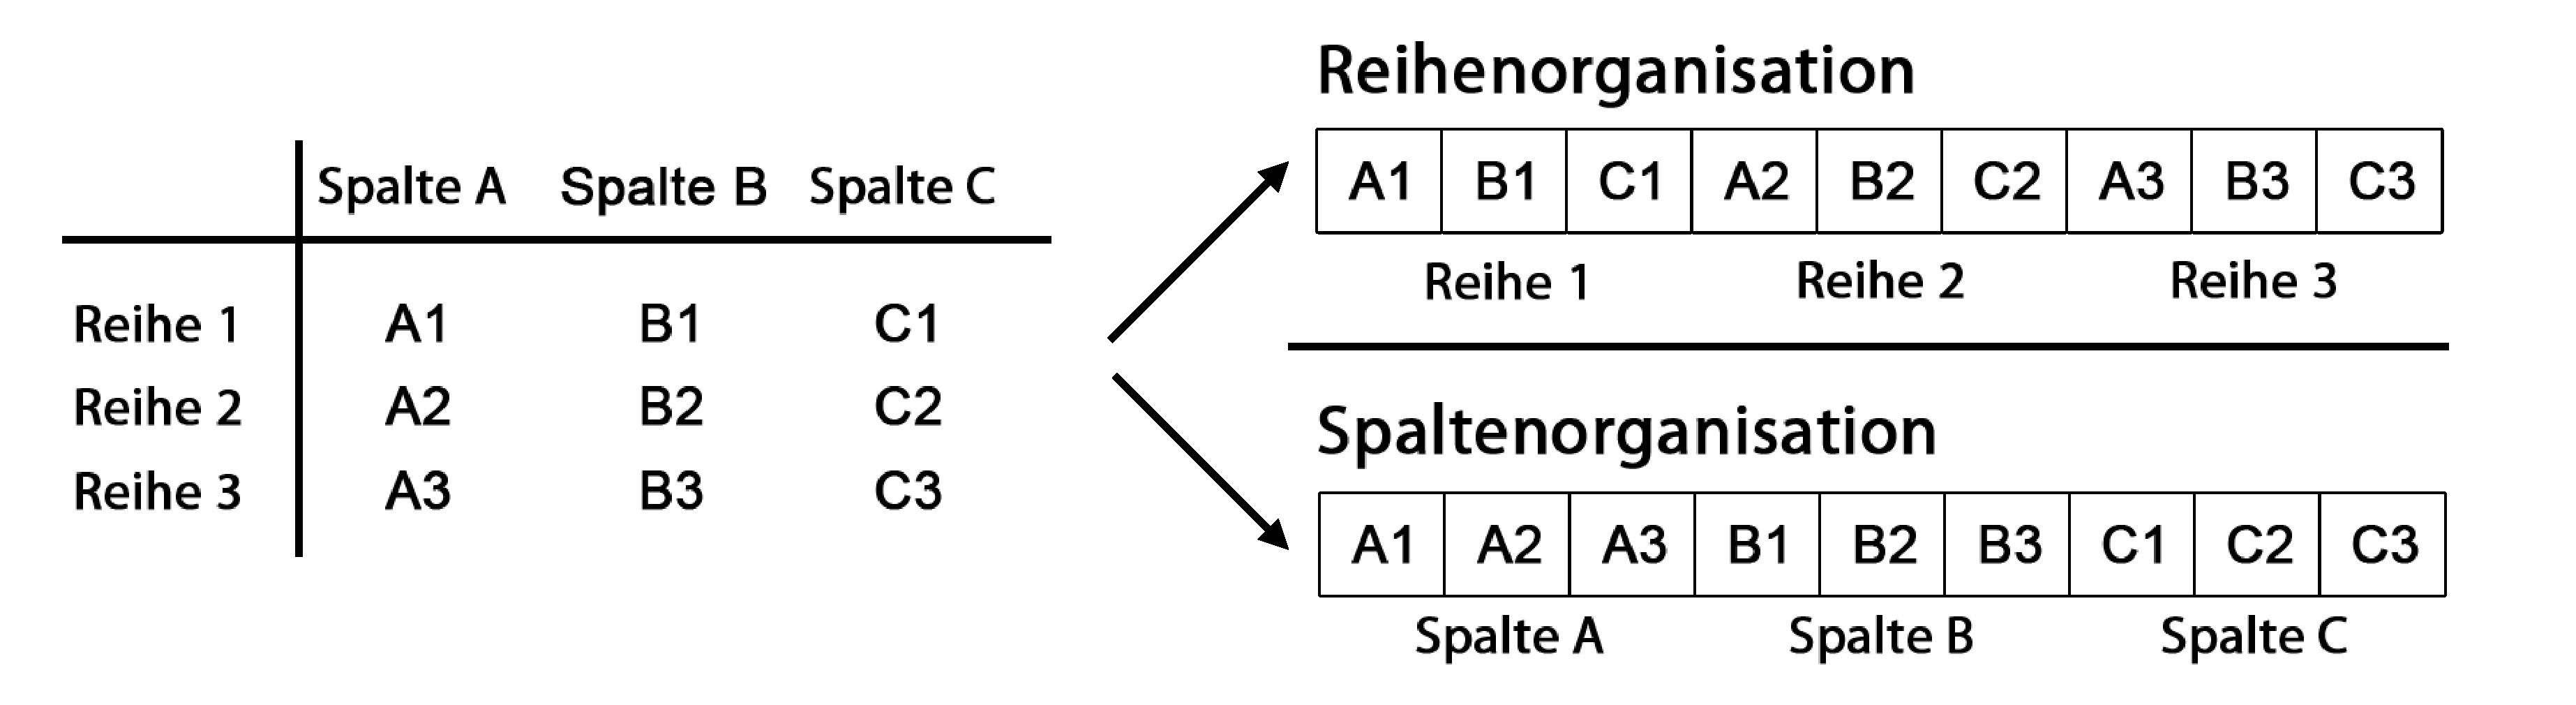
\includegraphics[width=15cm]{images/in-memory-row-column.pdf}
\caption
[Vergleich zwischen der Reihen- und Spaltenorganisation von Daten]
{Vergleich zwischen der Reihen- und Spaltenorganisation von Daten, Darstellung in Anlehnung an \seCite{}{S.13}{Kle.10} \label{fig:vergleich_spalte_zeile}}
\end{figure}

Die zeilenbasierte Organisation ist von Vorteil, wenn auf einzelne Datensätze komplett zugegriffen werden soll. Die spaltenbasierte Organisation ist bei Tabellen mit einer hohen Anzahl an Spalten und bei spaltenbasierten Operationen wie der Aggregation oder der Suche überlegen. Durch die Unterstützung von beiden Organisationsformen kann die jeweils beste Form gewählt werden.\seFootcite{vgl.}{S.13f}{Kle.10}

Veränderungen in einem Datensatz einer Tabelle können auf Wunsch nicht in dem Eintrag der Tabelle direkt geändert, sondern nur die Differenzen an die Tabelle angefügt werden. Dadurch bleibt die Information, wie sich der Datensatz im Laufe der Zeit verändert hat, erhalten und kann in späteren Auswertungen als weitere Information hinzugezogen werden. Zusätzlich ist das Anfügen einer Veränderung schneller durchzuführen als die Veränderung eines bestehenden Datensatzes.\seFootcite{vgl.}{S.109f}{PZ.11}

Zu den genannten Veränderungen wird in Anwendungen, die auf Basis von SAP HANA entwickelt werden, versucht, ein Teil der Anwendungslogik schon auf der Datenbank selbst zu berechnen.\seFootcite{vgl.}{S.155f}{PZ.11} Erreicht wird dies durch die Erweiterung der Abfragesprache \gls{sql} zu \gls{glos:sqlscript}. Mit \gls{glos:sqlscript} ist es unter anderem durch das Hinzufügen von Datentypen, Prozeduren und Operationen möglich, Anwendungslogik abzubilden. Diese Berechnungen können von der Datenbank durch Parallelisierung sehr schnell durchgeführt werden.\seFootcite{vgl.}{S.9f}{SQLScript.11} Als Resultat kann die Datenübertragung zwischen dem \gls{dbms} und der Anwendung verringert werden. Es muss nur noch das Ergebnis und nicht die Datensätze, auf denen das Ergebnis basiert, übertragen werden. Zusätzlich wird die Komplexität der Anwendung verringert, da ein Teil der Logik von dem \gls{dbms} übernommen wird.

\subsubsection{Oberon}
Als Oberflächentechnologie wird für das \gls{saplrm} das Oberon Framework genutzt. Es wurde ursprünglich als Oberfläche für \gls{glos:bydesign} entwickelt und wird jetzt auch für weitere Anwendungen, unter anderem für Anwendungen, die auf SAP HANA und \gls{ngap} basieren, verwendet.\seFootcite{vgl.}{}{Oberon-A} Ein Beispiel einer mit dem Oberon Framework umgesetzte Oberfläche ist in \vref{fig:oberon} zu sehen.

\begin{figure}[ht]
\centering
\setlength{\unitlength}{1mm}
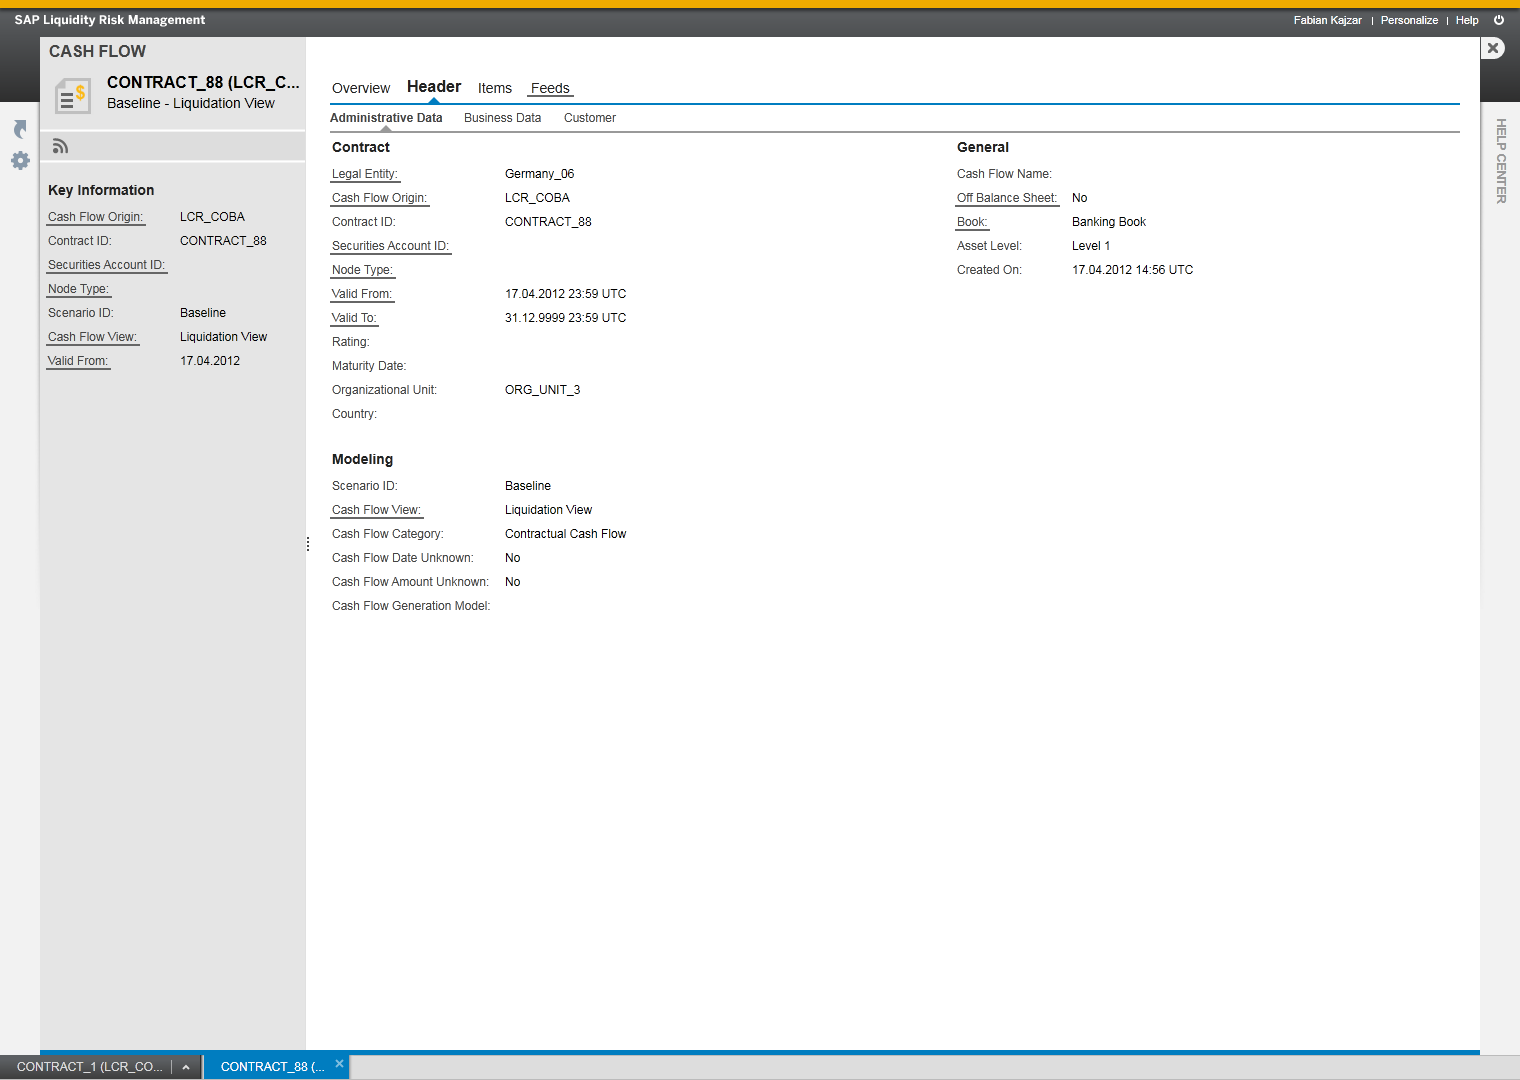
\includegraphics[width=15cm]{images/OberonUI-crop.png}
\caption{Darstellung eines Zahlungsstrom-Eintrags mit dem Oberon Framework\label{fig:oberon}}
\end{figure}

Oberflächen werden mit dem Oberen Framework mit der Programmiersprache C\# und Microsoft Silverlight\footnote{Microsoft Silverlight -- http://www.microsoft.com/silverlight/} entwickelt. Silverlight ist eine Technologie von Microsoft, die als Plug-in für verschiedene moderne Browser verfügbar ist und die Entwicklung von \gls{glos:ria} unterstützt. Die \gls{glos:ria} stellt dabei die erste Schicht der drei Schichtenarchitektur von Anwendungen dar. Die weiteren Schichten, die Anwendungslogik und die Persistenz, werden von \gls{ngap} und SAP HANA übernommen.\seFootcite{vgl.}{}{Oberon-A}

Das Oberon Framework ist als Standardframework ausgelegt und versucht, möglichst viele Anforderungen abzudecken. Dadurch soll es in vielen Produkten verwendet werden können. Allerdings ist es sehr wahrscheinlich, dass spezielle Anforderungen eines bestimmten Bereichs nicht mit dem Oberon Framework abgedeckt werden können. In diesem Fall müssen eigene Lösungen für die Anforderungen entwickelt werden.\seFootcite{vgl.}{}{Oberon-A}

\subsection{Berechnungskomponente}
\label{sec:berechnungskomponente}
Die Berechnungskomponente stellt den wichtigsten Teil des \gls{saplrm} dar. Mit ihr werden alle Berechnungen im Umfeld des Liquiditätsrisikomanagements zentral durchgeführt. Die Berechnung findet auf Basis von Liquiditätsgruppen statt. Mit Hilfe von Liquiditätsgruppen werden sowohl aggregierte Zahlungsströme als auch Kennzahlen einheitlich berechnet. Liquiditätsgruppen können in Polyhierarchien angeordnet werden. Dabei handelt es sich um eine Hierarchie, bei der ein Element mehrere übergeordnete Elemente haben kann. Dadurch können Berechnungen modular aufgebaut, wiederverwendet und einfach nachvollzogen werden. Das Abbilden von komplexen Berechnungsvorschriften wird erleichtert.\seFootcite{vgl.}{S.38}{LRM-PPT.12} Eine Hierarchie ist in \vref{fig:liquigruppe_hierarchie} zu sehen.

\begin{figure}[ht]
\centering
\setlength{\unitlength}{1mm}
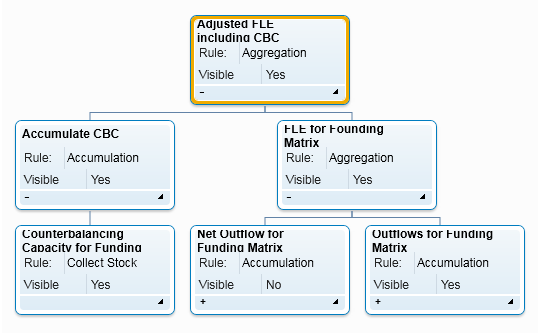
\includegraphics[width=10cm]{images/liquigruppe_hierarchie.PNG}
\caption{
Beispiel für die hierarchische Anordnung von Liquiditätsgruppen
\label{fig:liquigruppe_hierarchie}}
\end{figure}

Es existieren zwei Arten von Liquiditätsgruppen: Die Datenbankselektion und die Berechnung. Die Datenbankselektion bildet immer den Ursprung einer Berechnung. Dabei werden einzelne Zahlungsströme nach festgelegten Selektionskriterien ausgewählt und nach Bedingungen zusammengefasst. Mögliche Selektionskriterien sind der zugrunde liegende Produkttyp des Zahlungsstroms, wie zum Beispiel verzinsliches Wertpapier, oder das entsprechende Finanzrating, zum Beispiel AAA. Gleichzeitig findet eine Währungsumwandlung in eine einheitliche Zielwährung statt. Mehrere Zahlungsströme werden in Abhängigkeit ihrer Fälligkeit in Behältern zusammengefasst. Diese Behälter werden von dem festgelegten Laufzeitband definiert.\seFootcite{vgl.}{S.40}{LRM-PPT.12}

Ein Laufzeitband ist eine spezielle Einteilung der Zeitachse. Der Grund für die Einführung von Laufzeitbändern liegt in der späteren Auswertung der berechneten Werte. Dabei ist für naheliegende Zeiträume, zum Beispiel die nächste Woche, der entsprechende Wert an jedem einzelnen Tag entscheidend. Für den weiteren Horizont, zum Beispiel den Zeitraum zwischen drei und fünf Jahren, ist nicht jeder einzelne Tag entscheidend. Es reichen hier aggregierte Werte, zum Beispiel nach Monat oder Jahr. Somit kann in eine Auswertung sowohl die aktuelle Situation begutachtet werden, als auch die langfristigen Auswirkungen, ohne dass die Auswertung unübersichtlich wird. Jeder Eintrag entspricht dabei einem Behälter. Die Anzahl und Größe der Behälter ist in einem Laufzeitband definiert.\seFootcite{vgl.}{S.44}{LRM-PPT.12} Ein Beispiel für ein Laufzeitband ist in \vref{fig:laufzeitband} dargestellt.

\begin{figure}[ht]
\centering
\setlength{\unitlength}{1mm}

\includegraphics[width=15cm]{images/Abbildung4-Laufzeitband.pdf}
\caption{Mögliche Ausprägung eines Laufzeitbandes\label{fig:laufzeitband}}
\end{figure}

Neben der Datenbankselektion existiert die Liquiditätsgruppenart Berechnung. Dabei werden aggregierte Zahlungsströme nach verschiedenen Regeln verrechnet. Zur Verfügung stehende unter anderem Addition, Subtraktion, Multiplikation und Division. 

Generell hat eine Liquiditätsgruppe genau einen Output-Parameter, eine Berechnungsregel und kann zusätzlich mehrere Input-Parameter besitzen. Die Berechnung innerhalb einer Liquiditätsgruppe kann von szenarioabhängigen Variablen beeinflusst werden. Damit lassen sich zum Beispiel erwartete Kreditausfälle simulieren. Über diese Variablen werden die Szenarien umgesetzt. Mehrere Variablenausprägungen legen ein Szenario fest.\seFootcite{vgl.}{S.39 und S.45}{LRM-PPT.12}

\label{sec:berechnungskomponente:parameter}
Zur Laufzeit wird die Berechnungskomponente mit vier Parametern aufgerufen. In dem ersten Parameter werden eine oder mehrere Liquiditätsgruppen festgelegt, von denen später das Ergebnis zurückgeliefert wird. Ein weiterer Parameter legt den Stichtag fest, nach dem die Zahlungsströme ausgewählt werden. Jede Berechnung wird immer auf Basis von einem Laufzeitband durchgeführt, welches die Behälter festlegt, in die die Ergebnisse zusammengefasst werden. Schließlich wird noch eine Zielwährung festgelegt, in die alle Zahlungsströme umgerechnet werden.

Das Resultat der Berechnung ist jeweils der Output der festgelegten Liquiditätsgruppen. Zur Berechnung der Gruppen müssen in der Regel im Hintergrund weitere Liquiditätsgruppen berechnet werden, die allerdings nicht als Ergebnis zurückgeliefert werden. Während einer Berechnung werden Ergebnisse von Gruppen, die schon einmal berechnet wurden, zwischengespeichert, um Rechenaufwand zu sparen. Die Gruppen, die berechnet werden müssen, können aus der Hierarchie der entsprechenden Liquiditätsgruppe abgelesen werden.\seFootcite{vgl.}{S.44 und S.47}{LRM-PPT.12}

\section{BusinessObjects Xcelsius}
\label{sec:xcelsius}
\subsection{Überblick und Funktionsumfang} 
\gls{xcelsius} ist ein Teil der SAP BusinessObjects-Portfolio. Dabei handelt es sich um Anwendungen, mit denen Daten in einem Unternehmen analysiert und ausgewertet werden können. \gls{xcelsius} ist davon ein Tool zur Visualisierung von Daten durch die Erstellung von interaktiven Dashboards.

Dazu bietet es viele Möglichkeiten um Daten visualisieren und interaktiv beeinflussen zu können. Neben 20 Diagrammtypen, darunter unter anderem Linien-, Kreis-, Balken- und Flächendiagramme, stehen Schaltflächen zur Manipulation, wie zum Beispiel Schieberegler, Optionsfelder und Drehknöpfe, zur Verfügung. Zusätzlich können Kartenelemente zur Darstellung von Geoinformationen genutzt werden und Bilder und Texte unterstützend in ein Dashboard eingebunden werden. Viele Komponenten bieten zusätzlich Einstellungsmöglichkeiten, durch die das Aussehen oder das Verhalten angepasst werden kann.\seFootcite{vgl.}{S.31f und S.229f}{Egg.09}

Die Daten, auf denen die Visualisierungen in \gls{xcelsius} basieren, werden durch die Integration von Microsoft Excel verwaltet. Excel steht dabei in vollem Umfang zur Verfügung. Es können sowohl Berechnungen, als auch Formatierungen mit Excel durchgeführt werden. In \gls{xcelsius} wird Excel als Schnittstelle zwischen der Datenbeschaffung aus verschiedensten Quellen und der eigentlichen Visualisierung genutzt. Alle Daten, die visualisiert werden sollen, werden in ein Tabellenblatt von Excel geschrieben und von dort aus ausgelesen. Die Daten können demnach vor der Darstellung in Excel beliebig bearbeitet werden.\seFootcite{vgl.}{S.32 und S.236}{Egg.09} 

Die gesamte Erstellung eines Dashboards findet nach dem \gls{wysiwyg}-Prinzip statt. Der Anwender sieht schon während der Erstellung, wie das Ergebnis aussieht. Durch die Verwendung von Excel und dem Umsetzen des \gls{wysiwyg}-Prinzips benötigen Nutzer meist nur eine geringe Einarbeitungszeit und die Bedienung kann als intuitiv beschrieben werden. Besondere Programmiersprachenkenntnisse sind für die Erstellung von Dashboards nicht erforderlich.\seFootcite{vgl.}{S.32 und S.239}{Egg.09}

Die mit \gls{xcelsius} erstellten Dashboards werden mit Hilfe der Adobe Flex Technologie dargestellt. Dadurch ist kein spezieller Server oder ein \gls{dbms} notwendig. Es wird nur das Flash-Plug-in benötigt. Außerdem muss für die Darstellung keine Netzwerkverbindung zu einem Server oder dem Internet vorhanden sein. Zusätzlich können Dashboards in verschiedene Formate exportiert werden, um sie so in Microsoft PowerPoint-Präsentationen oder auf Internetseiten einzubinden.\seFootcite{vgl.}{S.31f und S.230}{Egg.09}

Als Datenquellen für ein Dashboard stehen mehrere Möglichkeiten zur Verfügung. Zum einen können Daten einfach in das Excel kopiert werden. Es ist auch möglich, ein \gls{bw}-System direkt anzuschließen, oder Daten über Webservices zu beziehen. Hierzu wird das \gls{xml}-Format verwendet. Außerdem existieren weitere Möglichkeiten, mit dem Dashboards zum Beispiel untereinander Daten austauschen können.\seFootcite{vgl.}{S.283f}{Egg.09}

\subsection{Bedienungskonzept}
Der vorgesehene Ablauf des Erstellens von Dashboards soll an dem Beispiel der Absatzzahlen von Produkten verdeutlicht werden. Zunächst soll jedoch die Oberfläche von \gls{xcelsius} dargestellt werden.

Die Oberfläche von \gls{xcelsius} lässt sich in vier Bereiche aufteilen. Die Bereiche sind in \vref{fig:xcelsius_ui_aufbau} dargestellt. Der Bereich A zeigt die Zeichenfläche, also das eigentliche Dashboard an. Auf der Zeichenfläche können Komponenten beliebig platziert werden. Alle verfügbaren Komponenten werden in dem Bereich B auf der linken Seite nach Kategorien geordnet dargestellt. Um eine Komponente auf der Zeichenfläche zu platzieren, wählt der Nutzer die Komponente aus und platziert sie per Drag \& Drop auf der Zeichenfläche. 

\begin{figure}[ht]
\centering
\setlength{\unitlength}{1mm}
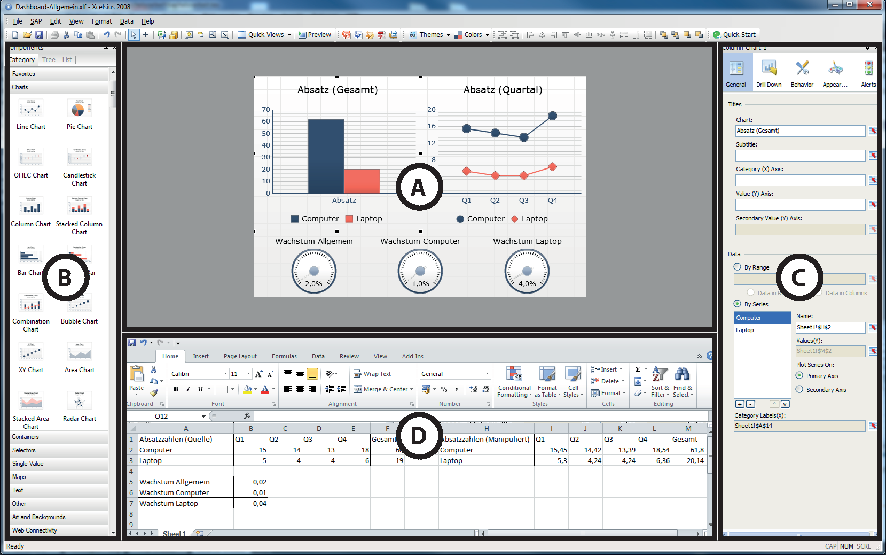
\includegraphics[width=15cm]{images/Abbildung5-Xcelsius-Oberflaeche-AI.pdf}
\caption{Die Oberfläche von BusinessObjects Xcelsius\label{fig:xcelsius_ui_aufbau}}
\end{figure}

Viele Komponenten bieten Einstellungsmöglichkeiten an, mit denen das Verhalten und das Aussehen der Komponente festgelegt werden kann. Wird eine Komponente auf der Zeichenfläche ausgewählt, werden alle verfügbaren Eigenschaften in Bereich C auf der rechten Seite dargestellt. Eigenschaften einer Komponente stellen oft die Daten dar, die die Komponenten anzeigen soll. Alle Daten werden in Bereich D festgelegt. Die Verbindung zwischen der Datenhaltung (Microsoft Excel in Bereich D) und der Darstellung (Zeichenfläche in Bereich A) von \gls{xcelsius} erfolgt durch das Referenzieren von Zellen oder Zellenbereichen über die Eigenschaften einer Komponente (Bereich C).\seFootcite{vgl.}{S.229}{Egg.09}

Für das Dashboard der Absatzzahlen in \vref{fig:xcelsius_ui_beispiel} werden die Daten in das Tabellenblatt eingetragen. Diese Daten können entweder fest eingegeben werden, meistens werden sie aber dynamisch über eine Datenquelle, zum Beispiel einen Webservice, in das Tabellenblatt geschrieben. In dem Beispiel wurden die Absatzzahlen fest in den Zellenbereich A eingetragen. 

Als nächstes können in Excel Berechnungen durchgeführt werden. In dem Beispiel wird die Summe der Absatzzahlen pro Jahr durch eine Formel berechnet. Um die Interaktivität von Dashboards zu zeigen, soll der Nutzer die Möglichkeit haben, die Auswirkungen von verschiedenen Wachstumsraten interaktiv zu sehen. Dazu werden die veränderten Absatzzahlen (Bereich B) auf Basis der Quelldaten in Bereich A und den Wachstumsdaten in Bereich C berechnet.\seFootcite{vgl.}{S.229f}{Egg.09}

\begin{figure}[ht]
\centering
\setlength{\unitlength}{1mm}
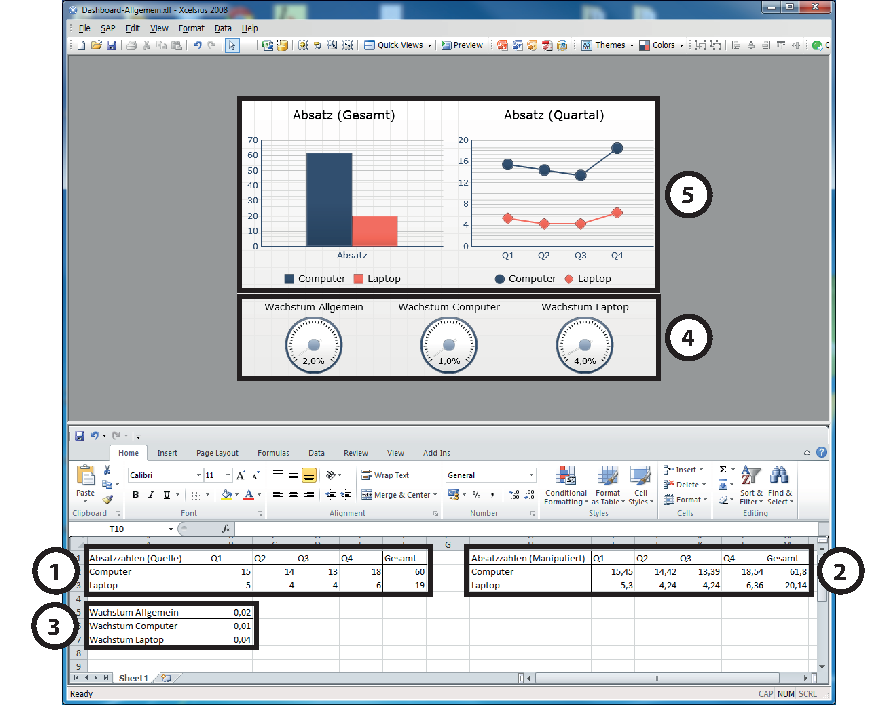
\includegraphics[width=15cm]{images/Abbildung6-Visualisierung-Absatz-Xcelsius-AI.pdf}
\caption{Visualisierung von Absatzzahlen in BusinessObjects Xcelsius\label{fig:xcelsius_ui_beispiel}}
\end{figure} 

Schließlich werden auf der Zeichenfläche zwei Diagramme, ein Säulendiagramm und ein Liniendiagramm in Bereich E festgelegt. Sie beziehen ihre Daten aus Bereich B. Die Wachstumsraten können mit drei Drehknöpfen in Bereich D festgelegt werden. Die Werte der Drehknöpfe sind mit den Zellen in Bereich C verknüpft. Dreht der Nutzer an einem Drehknopf, wird der aktualisierte Wert in die Zelle in Bereich C geschrieben. Da die Datenquelle der Diagramme mit Bezug auf die Wachstumswerte berechnet wird, verändern sich die Diagramme dynamisch. Das Prinzip ist schematisch noch einmal in \vref{fig:xcelsius_ablauf_schema} dargestellt. So ist es möglich, mit einfachen Mitteln, interaktive Dashboards zu erstellen.\seFootcite{vgl.}{S.237}{Egg.09}

\begin{figure}[ht]
\centering
\setlength{\unitlength}{1mm}
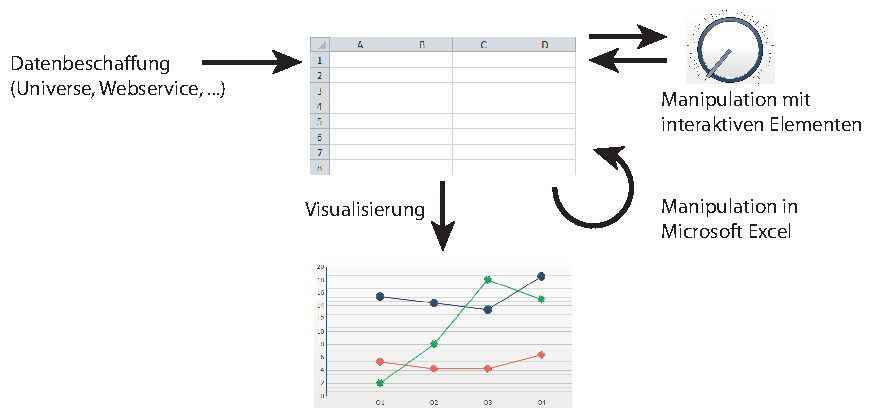
\includegraphics[width=15cm]{images/Abbildung4-Arbeitsweise-Xcelsius.pdf}
\caption{Schematische Darstellung der Arbeitsweise von BusinessObjects Xcelsius\label{fig:xcelsius_ablauf_schema}}
\end{figure}

\subsection{Architektur}
\gls{xcelsius} basiert auf dem \gls{glos:netFramework} von Microsoft und ist in weiten Teilen in C++ geschrieben. Neben C++ wird \gls{glos:actionscript} und das Adobe Flex Framework für die Benutzeroberfläche eingesetzt. Die Architektur von \gls{xcelsius} ist modular aufgebaut und besteht aus mehreren Teilen. Ein Überblick ist in \vref{fig:xcelsius_architektur} dargestellt.

\begin{figure}[ht]
\centering
\setlength{\unitlength}{1mm}
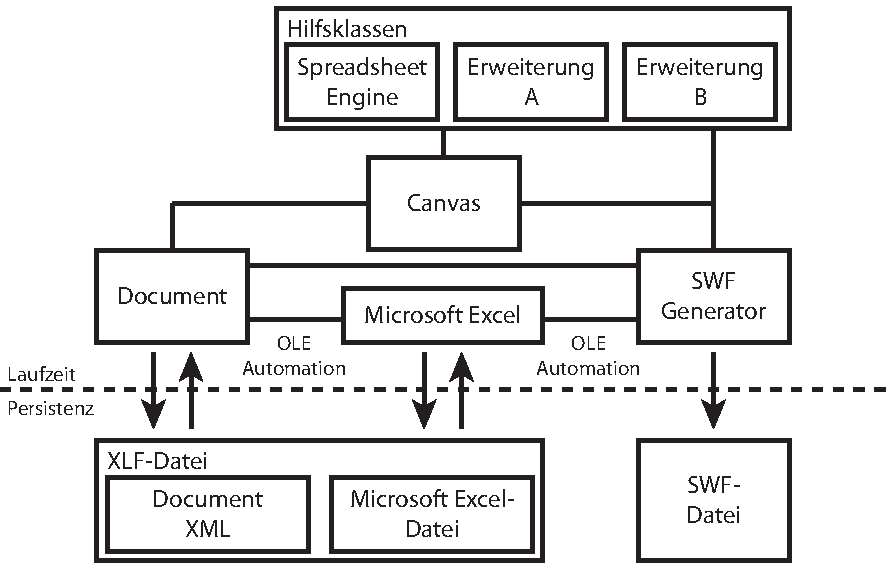
\includegraphics[width=15cm]{images/Abbildung5-Architektur-Xcelsius.pdf}
\caption{Architektur von BusinessObjects Xcelsius\label{fig:xcelsius_architektur}}
\end{figure}

Das zentrale Element ist das \class{Document}. Dabei handelt es sich um ein Objektmodell, das den aktuellen Zustand des Dashboards repräsentiert. Für die Darstellung wird das \class{Canvas} verwendet, welches in \gls{glos:actionscript} geschrieben ist. Die \class{Canvas}-Komponente nutzt dabei mehrere Hilfskomponenten. Dabei handelt es sich um die Komponenten, die später auf dem Dashboard platziert werden können. Diese Komponenten sind auch der Ansatzpunkt für spätere Erweiterungen. Eine Erweiterung ist intern eine zusätzliche Hilfskomponente.

An das \class{Document} ist mittels OLE Automation Microsoft Excel angebunden. OLE Automation ist eine Schnittstelle für die Kommunikation zwischen Prozessen. Speichern und Laden eines Dashboards übernimmt die XLF-Komponente. Diese erstellt oder lädt eine \gls{xcelsius} File (.xlf), welches intern aus dem Document im \gls{xml}-Format und einer Excel-Datei besteht.

Für den Export von erstellten Dashboards existiert der \class{SWF Generator}. Aus dem \class{Document} und den Daten und Formeln, die in Microsoft Excel erstellt wurden, wird eine .swf-Datei generiert. In dieser werden nun alle Berechnungen, die bis jetzt von Microsoft Excel übernommen wurden, von der Hilfskomponente \class{SpreadsheetEngine} berechnet.\seFootcite{vgl.}{}{Xcelsius-Arch.09}

\subsection{Erweiterungsmöglichkeiten}

Durch die Einstellungsmöglichkeiten der einzelnen Komponenten und die Einbindung des vollen Funktionsumfangs von Microsoft Excel ist \gls{xcelsius} von sich aus sehr flexibel. Zusätzlich dazu existiert noch ein \gls{glos:sdk} mit dem komplett eigene Komponenten erstellt werden können. Dadurch ist es möglich, \gls{xcelsius} um nahezu beliebige Funktionen zu erweitern.

Die Erweiterungen, die mit dem \gls{glos:sdk} programmiert werden können, müssen auf dem Adobe Flex SDK 2.0.1 basieren. Die Programmiersprache ist \gls{glos:actionscript}. Es können drei verschiedene Typen von Erweiterungen mit dem \gls{glos:sdk} entwickelt werden. Dabei handelt es sich um visuelle Komponenten, die später auf dem erstellten Dashboard dargestellt werden, um Datenverbindungen oder eine Erweiterung der Steuerungslogik von Excel.\footnote{\seCite{vgl.}{S.229}{Egg.09} \seCite{und}{S.3f}{Xcelsius-SDK.08}} Erweiterungen in Form einer visuellen Komponente oder für die Steuerungslogik von Excel spielen für die Arbeit keine Rolle.

Entscheidend für diese Bachelorarbeit ist die Datenverbindung. Dabei handelt es sich um Erweiterungen, die später auf den erstellten Dashboards nicht sichtbar sind. Während der Erstellung der Dashboards werden die Datenverbindungen konfiguriert, um dann später im Hintergrund aktiv zu sein. Eine typische Aufgabe einer Datenverbindung ist das Schreiben von Daten aus beliebigen Quellen in das Tabellenblatt des Dashboards. Von dort aus können die Daten dann in \gls{xcelsius} genutzt werden.

Das Ergebnis der Entwicklung einer Datenverbindung ist dann eine .swf-Datei. Sie besteht aus einer einfache Oberfläche für die Konfiguration und in \gls{glos:actionscript} geschriebene Klassen, in denen die Logik umgesetzt ist. Die Datei wird, in Verbindung mit Informationen zu der Komponente, wie zum Beispiel Name, Version, Typ und Entwickler, mit dem \gls{xcelsius} \gls{glos:sdk} zu einem \gls{xcelsius} Plug-in zusammengefügt. Das Resultat kann dann in \gls{xcelsius} importiert und die Komponenten so genutzt werden.\footnote{\seCite{vgl.}{S.283f}{Egg.09} \seCite{und}{S.6}{Xcelsius-SDK.08}}

\section{Zusammenfassung}
In diesem Kapitel wurde ein Einblick in zwei zentrale Anwendungen der Bachelorarbeit gegeben -- dem \gls{saplrm} und \gls{xcelsius}. Wichtig für den weiteren Verlauf der Bachelorarbeit ist zum einen die Berechnungskomponente des \gls{saplrm}, da diese als Ergebnis dieser Bachelorarbeit in weiteren Anwendungen genutzt werden soll. Zum anderen wurde \gls{xcelsius} im Hinblick auf das Bedienungskonzept und der Erweiterbarkeit genauer untersucht. Die guten Erweiterungsmöglichkeiten und das offene Bedienkonzept spielen für den weiteren Verlauf eine entscheidende Rolle.

\chapter{Spezifikation der Zwischenschicht}
\label{sec:spezifikation}

\section{Einleitung}
In diesem Kapitel wird die Spezifikation der Zwischenschicht durchgeführt. Dazu wird in einem ersten Schritt die Ausgangssituation dargestellt und auf Verbesserungspotential untersucht. Anschließend wird die angestrebte Zielsituation skizziert. Ausgehend von der Zielsituation werden dann in einem weitern Schritt die dafür notwendigen Anforderungen festgelegt. Diese dienen später zur Evaluation des Ergebnisses. Schließlich werden noch die wichtigsten Anwendungsfälle näher beschrieben, um so eine genauere Vorstellung von der Erweiterung zu erhalten.

\section{Ausgangssituation}
In dem derzeitigen Stand des \gls{saplrm} gibt es für die Analyse der aktuellen Liquiditätssituation einer Bank zwei Einstiegsmöglichkeiten. Es existiert die Kennzahlenanalyse und die Finanzierungsmatrix. Diese unterschieden sich in ihrer Nutzung.

Der Zweck der Kennzahlenanalyse ist die Darstellung von Kennzahlen, die nach einer festen Vorschrift berechnet werden können. Neben internen Kennzahlen, die eine Bank für sich selbst definiert hat, sind hier vor allem offizielle Kennzahlen von Bedeutung. Dazu gehören zum Beispiel im Rahmen von Basel III der \gls{glos:lcr} und der \gls{glos:nsfr}. Somit kann die Kennzahlenanalyse genutzt werden, um offizielle regulatorische Vorschriften zu überwachen. Die Darstellung der Kennzahlen ist ausschließlich in tabellarischer Form möglich. Ein Beispiel zeigt \vref{fig:lrm_istzustand_keyfigureanalysis}.

\begin{figure}[ht]
\centering
\setlength{\unitlength}{1mm}
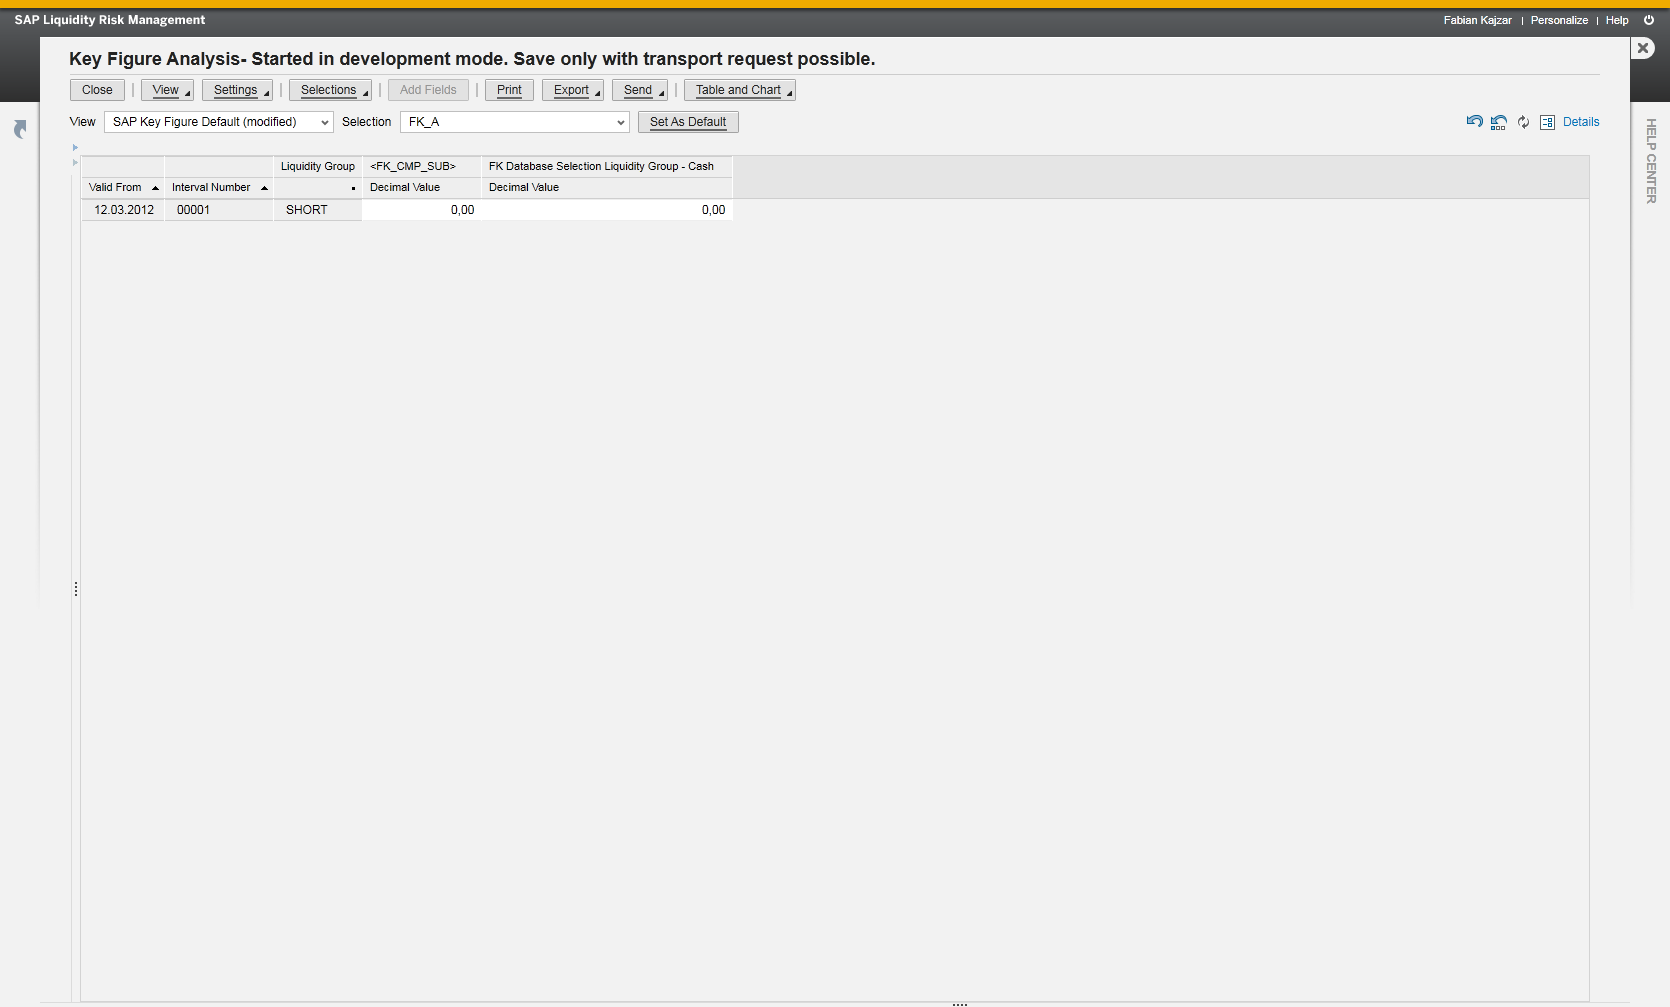
\includegraphics[width=15cm]{images/KeyFigureAnalysis_Example-crop.png}
\caption{Darstellung der Kennzahlenanalyse im \gls{saplrm}\label{fig:lrm_istzustand_keyfigureanalysis}}
\end{figure}

Neben der Kennzahlenanalyse existiert die Finanzierungsmatrix. Hier sollen nicht feste Kennzahlen dargestellt werden. Vielmehr wird die Möglichkeit geboten, die Liquiditätssituation der Bank frei zu analysieren. Sowohl die Finanzierungsmatrix, als auch die Kennzahlenanalyse, nutzen für die Berechnung der Werte die Berechnungskomponente. Bei der Finanzierungsmatrix hat der Nutzer die Möglichkeit, die Selektionskriterien in Form der nötigen Parameter für den Aufruf der Berechnungskomponente zur Laufzeit festzulegen. Die Darstellung ist hier auf ein Liniendiagramm festgelegt. \vref{fig:lrm_istzustand_fundingmatrix} zeigt die Finanzierungsmatrix.

\begin{figure}[ht]
\centering
\setlength{\unitlength}{1mm}
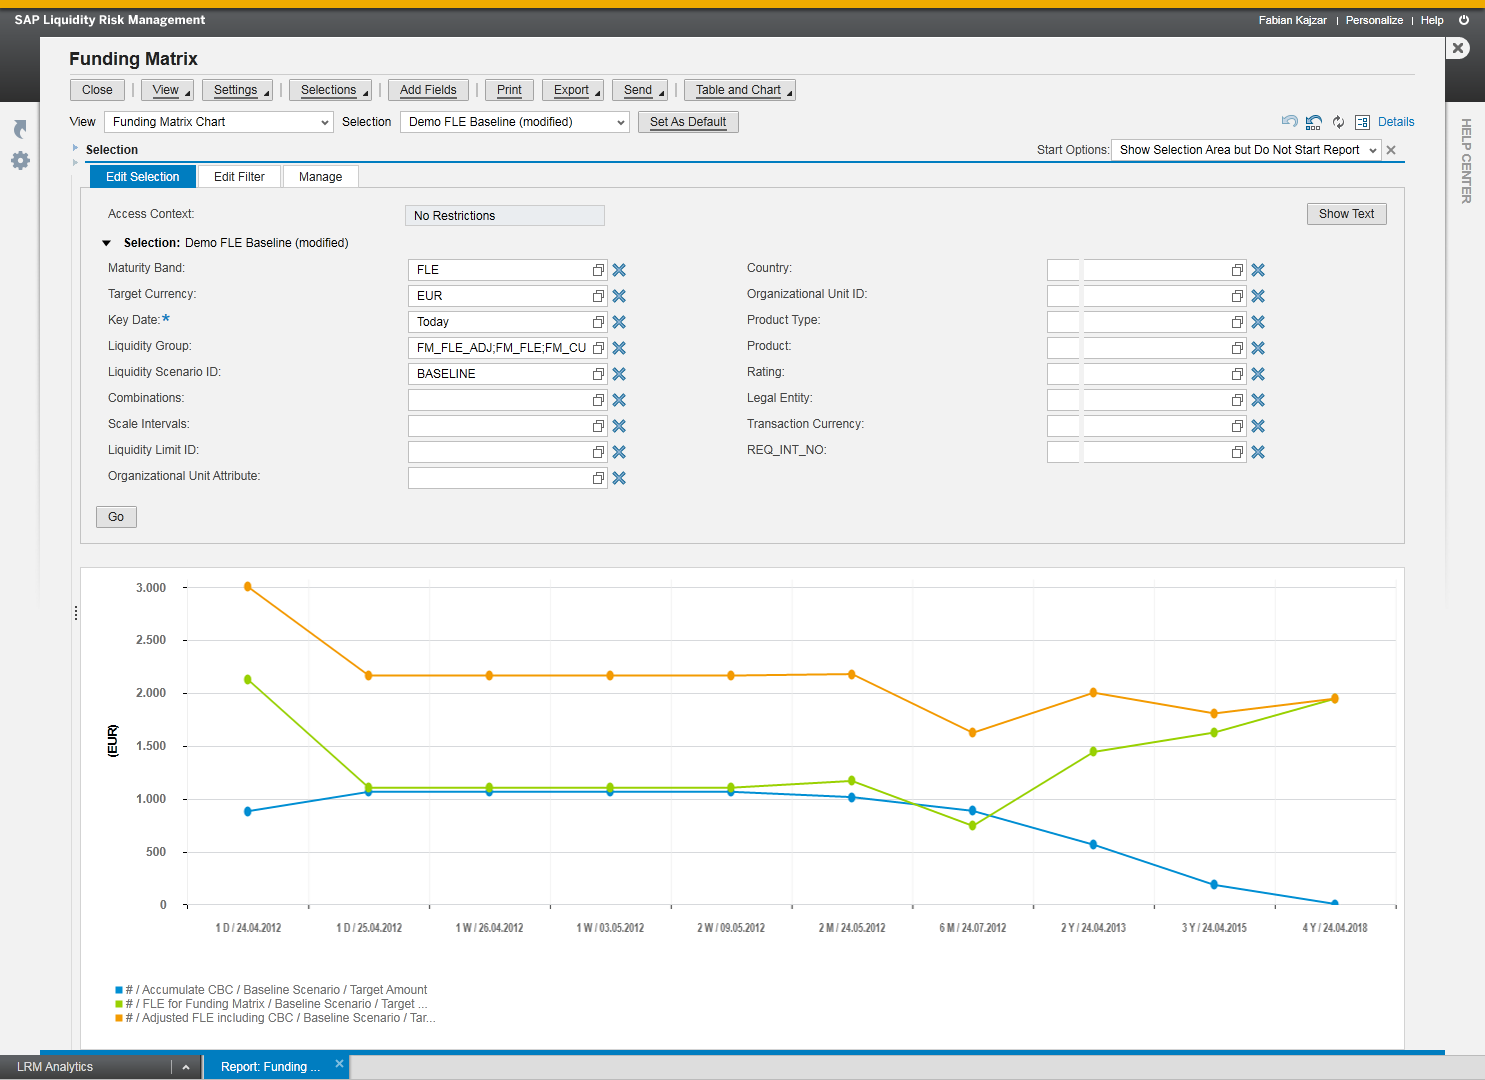
\includegraphics[width=15cm]{images/Funding_Matrix_Example-crop.png}
\caption{Darstellung der Finanzierungsmatrix im \gls{saplrm}\label{fig:lrm_istzustand_fundingmatrix}}
\end{figure} 

Allgemein ist festzustellen, dass in der aktuellen Version keine Möglichkeit besteht, die Ergebnisse der Berechnungen in irgendeiner Form in anderen Auswertungen, zum Beispiel Auswertungen, die die gesamte Situation der Bank beschreiben, einzubinden. Des Weiteren besteht bei der Darstellung der Ergebnisse keine Formatierungsmöglichkeit. Somit sind zum Beispiel Farbe, Form und Größe des Diagramms fest vorgegeben und nicht durch den Nutzer änderbar. Dies ist in der Nutzung des Oberon Frameworks begründet.

\section{Zielsetzung}
\label{sec:zielsetzung}

Im Rahmen dieser Bachelorarbeit sollen einige Limitierungen, die in der aktuellen Version des \gls{saplrm} vorhanden sind, aufgehoben werden. Hier ist vor allem die Bereitstellung von weiteren Alternativen zu nennen. Neben der Sicht auf die Liquiditätssituation der Bank durch die beiden Einstiegspunkte Kennzahlenanalyse und der Finanzierungsmatrix im \gls{saplrm} soll diese Auswertung mit Hilfe von weiteren Anwendungen durchgeführt werden können.

Durch die Anbindung von weiteren Anwendungen bietet sich die Möglichkeit, die Liquiditätssteuerung in die Gesamtsteuerung der Bank einzubinden. Ein Ziel ist es, in einen Bericht, der Daten zu der allgemeinen Situation der Bank anzeigt, auch Informationen über das Liquiditätsrisikomanagement aufzunehmen. Dadurch kann die Situation der Bank gesamtheitlich erfasst werden und Entscheidungen unter der Berücksichtigung von weiteren Informationen getroffen werden.

Simultan dazu können durch eine Anbindung des \gls{saplrm} an weitere Anwendungen die jeweiligen Vorteile der angebundenen Anwendung ausgenutzt werden. Hier ist zum Beispiel die Flexibilität in der Darstellung der Daten zu nennen. Wenn die Anwendung weitere grafische Visualisierungsmöglichkeiten bietet, können diese auf die Daten des \gls{saplrm} angewendet werden.

Insgesamt soll die Anbindung des \gls{saplrm} mit möglichst wenig erforderlichen Einstellungen konfigurierbar sein. Gleichzeitig ist es erstrebenswert, dass das Konzept der Anbindung und die Implementierung, die im Rahmen der Bachelorarbeit entwickelt wird, in der grundsätzlichen Idee und Architektur auch auf weitere Anwendungen übertragen werden kann.

\section{Anforderungen}
\label{sec:anforderungen}
Für die Erweiterung werden im Rahmen der Spezifikation einige Anforderungen definiert. Die Anforderungen werden zunächst in funktionale und nicht-funktionale Anforderungen unterteilt. 

Bei den funktionalen Anforderungen existieren die zwei folgenden Hauptanforderungen:

\begin{seToplist}{ XXXXX }

\item[\anfl{kpi}] \textbf{Einbindung von Kennzahlen} \newline
Die Erweiterung soll es ermöglichen, dass Kennzahlen, die im \gls{saplrm} mit Hilfe der Berechnungskomponente ermittelt werden und im Bereich der Kennzahlenanalyse zur Verfügung stehen, in weitere Anwendungen integriert werden und dort weiterverarbeitet werden können.

\item[\anfl{fundingMatrix}] \textbf{Freie Analyse der Liquiditätssituation} \newline
Mit der Erweiterung soll die Einbindung der Ergebnisse von beliebigen Liquiditätsgruppen ermöglicht werden. Die Liquiditätsgruppen sollen in Anlehnung an die Finanzierungsmatrix im \gls{saplrm} eingestellt werden und auf der Berechnungskomponente basieren. Neben den erforderlichen Parametern, wie zum Beispiel dem genutzten Laufzeitband und der Zielwährung sollen weitere Einschränkungsmöglichkeiten geboten werden, welche die Berechnungskomponente unterstützt.

\end{seToplist}

Durch die Umsetzung dieser beiden Anforderungen können die Ziele, die im \vref{sec:zielsetzung} festgelegt sind, erreicht werden. Dadurch bieten sich für den Nutzer bei der Auswertung und Analyse der Liquiditätssituation einer Bank zusätzliche Möglichkeiten.

Neben den funktionalen Anforderungen wurden auch nicht-funktionale Anforderungen identifiziert. Diese sollen im Folgenden näher erläutert werden:

\begin{seToplist}{ XXXXX }

\item[\anfl{uebertragbarkeit}] \textbf{Übertragbarkeit} \newline
Im Rahmen der Bachelorarbeit wird exemplarisch die Anbindung einer weiteren Anwendung zur Auswertung an das \gls{saplrm} implementiert. Das Konzept der Umsetzung soll dennoch auf weitere Anwendungen übertragen werden können.

\item[\anfl{korrektheit}] \textbf{Korrektheit der Ergebnisse} \newline
Die Daten, die mit Hilfe der Erweiterung in zusätzlichen Anwendungen verfügbar gemacht werden, müssen mit den Ergebnissen des \gls{saplrm} übereinstimmen. Nur wenn das sichergestellt ist, kann die Erweiterung sinnvoll genutzt werden.

%SAP LRM Abkürzung wg Zeilenumbruch erstetzt
\item[\anfl{erweiterbarkeit}] \textbf{Erweiterbarkeit} \newline
Das SAP LRM befindet sich aktuell noch in einer ersten Version in der Entwicklung. Weitere Versionen sind schon jetzt in Planung. Zusätzliche Funktionen und Möglichkeiten, die in einer Weiterentwicklung des SAP LRM eingeführt werden, sollen mit möglichst geringem Aufwand auch auf die Erweiterung übertragen werden können.

\item[\anfl{wartbarkeit}] \textbf{Wartbarkeit} \newline
Um die Folgekosten der Erweiterung, zum Beispiel im Hinblick auf die Beseitigung von Fehlern, möglichst gering zu halten, soll eine gute Wartbarkeit von Anfang an bei der Entwicklung beachtet werden.

\item[\anfl{sicherheit}] \textbf{Sicherheitsanforderungen} \newline
Die Erweiterungen wird Zugang zu den Daten des \gls{saplrm} bieten. Es handelt sich dabei um vertrauliche Daten, die Zugangsbeschränkungen unterliegen. Es muss sichergestellt sein, dass die Zugangsbeschränkungen eingehalten werden und Daten nicht von unberechtigten Personen ausgelesen werden können.

\item[\anfl{leistung}] \textbf{Leistung} \newline
Ein wichtiges Unterscheidungsmerkmal des \gls{saplrm} durch die Nutzung von SAP HANA ist die schnelle Analyse von Daten. Die Erweiterung soll die Geschwindigkeitsvorteile von SAP HANA auch in anderen Anwendungen verfügbar machen.

\end{seToplist}

Die Reihenfolge der Anforderungen spiegelt gleichzeitig auch die Priorität der Umsetzung wieder. Die wichtigsten Anforderungen sind \anfRef{anf:uebertragbarkeit}{} und \anfRef{anf:korrektheit}{}. \anfRef{anf:leistung}{} steht bei der Entwicklung nicht im Mittelpunkt.

\section{Anwendungsfälle}
Zum besseren Verständnis des Ziels der Erweiterung werden die Hauptanwendungsfälle im Folgenden näher beschrieben. Der Anwendungsfall 1\usecaseRef{useCase:1} konkretisiert die \anfRef{anf:kpi}{} und behandelt die Einsicht in wichtige Liquiditätskennzahlen einer Bank.

\useCase{1: Liquiditätskennzahl einsehen}{ \label{useCase:1}

\useCaseEntry{Ziel}{Liquiditätskennzahl der Bank einsehen}
\useCaseEntry{Vorbedingung}{Die Liquiditätskennzahl ist im \gls{saplrm} angelegt und verfügbar}
\useCaseEntry{Nachbedingung: Erfolg}{Die Liquiditätskennzahl kann eingesehen werden}
\useCaseEntry{Nachbedingung: Fehlschlag}{Anzeige einer Fehlermeldung}
\useCaseEntry{Akteure}{Controller, Manager}
\useCaseEntry{Auslösendes Ereignis}{Der Wert der Liquiditätskennzahl soll überprüft werden}

\textbf{Beschreibung}
\begin{seToplist}{ x 1 x }
\vspace*{-4mm}
\useCaseItem{1}{Die einzusehende Liquiditätskennzahl wird ausgewählt}
\useCaseItem{2}{Die Daten werden aus dem \gls{saplrm} ermittelt}
\useCaseItem{3}{Die Daten werden der Anwendung zur Verfügung gestellt}
\end{seToplist}

}

Der Anwendungsfall 2\usecaseRef{useCase:2} bezieht sich auf die \anfRef{anf:fundingMatrix}{}. Hierbei geht es um die freie Analyse der Liquiditätssituation einer Bank.

\useCase{2: Liquiditätssituation analysieren}{ \label{useCase:2}

\useCaseEntry{Ziel}{Liquiditätssituation der Bank analysieren}
\useCaseEntry{Vorbedingung}{Erforderliche Zahlungsströme, Liquiditätsszenarien, Liquiditätsgruppen und Laufzeitbänder sind im \gls{saplrm} angelegt und verfügbar}
\useCaseEntry{Nachbedingung: Erfolg}{Die Liquiditätssituation kann eingesehen werden}
\useCaseEntry{Nachbedingung: Fehlschlag}{Anzeige einer Fehlermeldung}
\useCaseEntry{Akteure}{Controller, Manager}
\useCaseEntry{Auslösendes Ereignis}{Es besteht Unklarheit über die Liquiditätssituation der Bank}

\textbf{Beschreibung}
\begin{seToplist}{ x 1 x }
\vspace*{-4mm}
\useCaseItem{1}{Der zu analysierende Zeitraum wird mit dem Laufzeitband festgelegt}
\useCaseItem{2}{Die Zielwährung der Analyse wird festgelegt}
\useCaseItem{3}{Das Liquiditätsszenario wird festgelegt}
\useCaseItem{4}{Die zu analysierenden Liquiditätsgruppen werden festgelegt}
\useCaseItem{5}{Die Daten werden aus dem \gls{saplrm} ermittelt}
\useCaseItem{6}{Die Daten werden der Anwendung zur Verfügung gestellt}
\end{seToplist}

\textbf{Erweiterungen}
\begin{seToplist}{ x 1 x }
\vspace*{-4mm}
\useCaseItem{4a}{Weitere Selektionsmerkmale, zum Beispiel nach Produkttyp oder Organisationseinheit werden festgelegt}
\useCaseItem{6a}{Die Daten werden in der Anwendung weiterverarbeitet}
\useCaseItem{6b}{Die Daten werden in der Anwendung visualisiert}
\end{seToplist}

}

\section{Zusammenfassung}
In diesem Kapitel wurde die angestrebte Zielsituation, die mit der Erweiterung erreicht werden soll, genauer beschrieben. Dafür wurden sowohl funktionale als auch nicht-funktionale Anforderungen festgelegt. Diese spielen am Ende der Bachelorarbeit noch eine wichtige Rolle. Sie stellen Kriterien dar, anhand deren die Erweiterung gemessen und bewertet werden kann. Schließlich wurde mit den zwei Hauptanwendungsfällen die grundlegende Interaktion mit der Erweiterung konkretisiert.

\chapter{Umsetzungsmöglichkeiten}

\section{Einleitung}
Dieses Kapitel greift die Ergebnisse der Spezifikation auf und untersucht verschiedene Möglichkeiten der Umsetzung. Dazu werden die in Frage kommenden Alternativen genauer dargestellt und die jeweiligen Vor- und Nachteile ermittelt. Durch einen abschließenden Vergleich wird dann eine Umsetzungsmöglichkeit für das weitere Vorgehen festgelegt.

\section{Rahmenbedingungen}
Bis zu diesem Zeitpunkt ist die Arbeit, mit Ausnahme der Vorstellung von \gls{xcelsius} in \vref{sec:xcelsius}, allgemein gehalten. Die Spezifikation beschreibt ein allgemeines Konzept für die Einbindung von Daten des \gls{saplrm} zur weiteren Analyse. Für das weitere Vorgehen soll das Konzept an dem konkreten Beispiel von \gls{xcelsius} umgesetzt werden. Der folgende Teil behandelt demnach die konkrete Anbindung von \gls{xcelsius} an das \gls{saplrm}. Gleichzeitig soll aber bei der Analyse und dem Entwurf die \anfRef{anf:uebertragbarkeit}{an die Übertragbarkeit } wenn möglich weiterhin beachtet werden.

\section{BusinessObjects Universum}
Eine Möglichkeit, externe Daten in \gls{xcelsius} zu integrieren, stellt BusinessObjects Universum dar. Dabei handelt es sich um eine Zwischenschicht, die zwischen dem Bereitsteller der Daten und dem Konsumenten geschaltet wird. Ein Universum ist eine semantische Ebene, die es ermöglicht, Daten zu konsumieren, ohne die technischen Aspekte der Datenbank kennen zu müssen.\seFootcite{vgl.}{S.48f}{Universe.06}


Es können Daten aus relationalen \gls{dbms}, die zum Beispiel in normalisierter Form vorliegen, und aus \gls{bw}-Systemen, die Daten zum Beispiel im Sternschema ablegen, konsumiert werden. Das Sternschema ist ein besonderes Datenmodell, welches besonders für Leseoperationen optimiert ist. Das Universum abstrahiert diese Daten auf Objekte, die dem Nutzer bereitgestellt werden.\seFootcite{vgl.}{S.49}{Universe.06}

Die Einbindung von Universen wird in \gls{xcelsius} standardmäßig unterstützt. Es könnte somit im \gls{saplrm} eine oder mehrere Datenbanktabellen erstellt werden, die mit den Ergebnissen der Berechnungskomponente gefüllt werden. Für diese Datenbanktabellen wird ein Universum erstellt, welches dann schließlich an \gls{xcelsius} angebunden wird. Ein Überblick ist in \vref{fig:umsetzung_universe} dargestellt.

\begin{figure}[ht]
\centering
\setlength{\unitlength}{1mm}
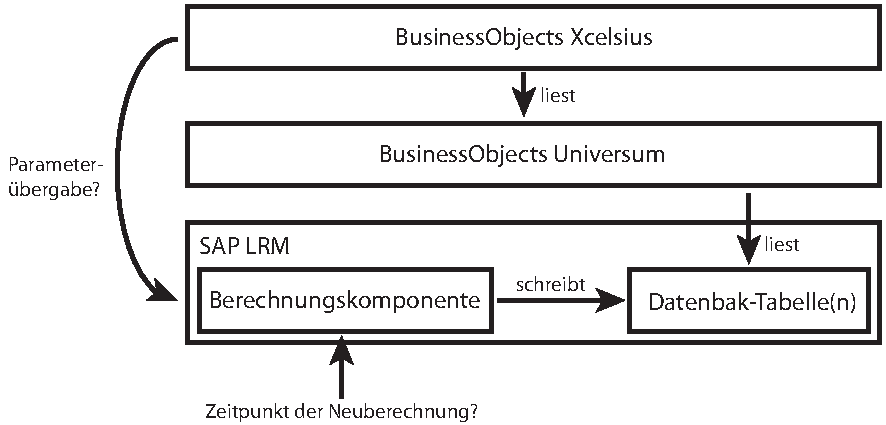
\includegraphics[width=15cm]{images/Abbildung9-Umsetzung-Universum.pdf}
\caption{Umsetzungsmöglichkeit der Erweiterung mittels BusinessObjects Universum \label{fig:umsetzung_universe}}
\end{figure}

Da ein Universum allerdings nur lesenden Zugriff auf die Daten bietet, stellt sich die Frage, wie eventuelle Selektionsparameter von \gls{xcelsius} an die Berechnungskomponente übergeben werden können. Zusätzlich muss die Berechnung durch die Berechnungskomponente manuell angestoßen werden, um die Tabelle mit den aktuellen Daten zu füllen. Eine automatische, periodische Berechnung, zum Beispiel durch einen eingeplanten Hintergrundprozess, würde stets veraltete Daten liefern.

Schließlich sind Universen nur für die Verwendung mit BusinessObjects Anwendungen ausgelegt. Das Kriterium der Übertragbarkeit in \anfRef{anf:uebertragbarkeit}{} kann somit nicht garantiert werden.

\section{Webservice}
%SAP LRM wg Blocksatzverletzung ersetzt
Eine weitere Möglichkeit stellen Webservices dar. Für die Umsetzung muss im SAP LRM der Webservice implementiert werden. In \gls{xcelsius} wird dieser Webservice aufgerufen und somit über den Webservice Daten konsumiert. Ein Überblick stellt \vref{fig:umsetzung_webservice} dar.

\begin{figure}[ht]
\centering
\setlength{\unitlength}{1mm}
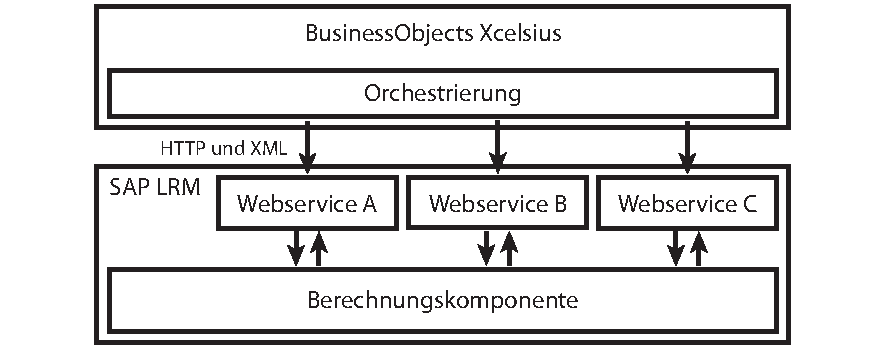
\includegraphics[width=15cm]{images/Abbildung10-Umsetzung-Webservices.pdf}
\caption{Umsetzungsmöglichkeit der Erweiterung mittels Webservices \label{fig:umsetzung_webservice}}
\end{figure} 

Dadurch, dass der Aufruf direkt im \gls{saplrm} entgegen genommen wird und nicht indirekt, zum Beispiel über ein Universum erfolgt, können eventuelle Selektionsparameter dynamisch übergeben werden. Auch das Problem mit veralteten Daten besteht nicht, da die Berechnung bei jedem Aufruf nach Bedarf durchgeführt werden kann.

Werden für die Umsetzung der Webservices offene Standards, wie zum Beispiel \gls{http} für die Übertragung oder \gls{xml} als Beschreibungssprache eingesetzt, können die Webservices auch von anderen Anwendungen verwendet werden. Dies ist für das Kriterium der Übertragbarkeit in \anfRef{anf:uebertragbarkeit}{} wichtig.

Außerdem kommt hinzu, dass bei dieser Umsetzungsmöglichkeit eine gute Modularisierung und Wiederverwendbarkeit erreicht werden kann. Die benötigte Funktionalität kann auf mehrere kleine Webservices aufgeteilt werden. Es entstehen voneinander unabhängige Teile, die leichter gewartet und unabhängig voneinander verwendet werden können. In \gls{xcelsius} müssen diese Teile dann orchestriert werden.

Teile des \gls{saplrm} wurden mit Hilfe eines Frameworks umgesetzt. Dieses bietet die Möglichkeit, bestimmte Klassen ohne zusätzlichen Programmieraufwand automatisch über einen Webservice bereitzustellen. Dazu zählen unter anderem die Liquiditätsszenarien und die Laufzeitbänder. Somit könnten Teile der Webservices ohne großen Aufwand umgesetzt werden.

Ein mögliches Risiko dieser Umsetzungsmöglichkeit stellt die \anfRef{anf:leistung}{an die Performance } dar. Der zusätzliche Aufwand für das Aufrufen von mehreren Webservices, in festgelegten Reihenfolgen und Abhängigkeiten, kann zu einer längeren Gesamtlaufzeit führen. Zusätzlich führt der Ausfall eines Teil-Webservices zur Funktionsunfähigkeit der gesamten Erweiterung.

\gls{xcelsius} bietet zwar eine Möglichkeit zur Einbindung von einzelnen Webservices, allerdings besteht standardmäßig keine Möglichkeit, mehrere Webservices zusammenzusetzen und zu orchestrieren. Dafür müsste eine eigene Erweiterung auf Basis des \gls{xcelsius} \gls{glos:sdk} entwickelt werden.

\section{Gegenüberstellung und Auswahl der Umsetzungsmöglichkeiten}
Für die Auswahl der im Rahmen der Bachelorarbeit angewendeten Umsetzungsmöglichkeit wurden die Vor- und Nachteile der Alternativen ermittelt und in \vref{table:vergleich_umsetzung} gegenübergestellt.

\begin{table}[ht]
\centering
\begin{tabular}{p{25mm}|p{55mm}|p{55mm}}
& \multicolumn{1}{c|}{\textbf{Vorteile}} & \multicolumn{1}{c}{\textbf{Nachteile}} \tabularnewline \hline
\begin{description}[leftmargin=0pt, topsep=0pt, itemsep=1pt] 
\item \textbf{Universum}
\end{description}
&
\begin{itemize}[leftmargin=*, topsep=0pt, itemsep=1pt] 
\item Standardmäßige Anbindung von Universen
\end{itemize}
&
\begin{itemize}[leftmargin=*, topsep=0pt, itemsep=1pt] 
\item zusätzliche Infrastruktur notwendig
\item Übertragbarkeit auf andere Anwendungen
\item Problem der dynamischen Übergabe von Parametern
\item Problem der Aktualisierung der berechneten Daten
\end{itemize}
\tabularnewline \hline
\begin{description}[leftmargin=0pt, topsep=0pt, itemsep=1pt] 
\item \textbf{Webservices}
\end{description}
&
\begin{itemize}[leftmargin=*, topsep=0pt, itemsep=1pt] 
\item Übergabe von Selektionsparametern einfach möglich
\item keine zusätzliche Infrastruktur erforderlich
\item gute Modularisierung und Übertragbarkeit
\item teilweise Bereitstellung von Webservices durch Framework
\end{itemize}
&
\begin{itemize}[leftmargin=*, topsep=0pt, itemsep=1pt] 
\item Komplexe Orchestrierung erforderlich
\item Performanceprobleme bei Web\-ser\-vice-\-Aufrufen
\item Ausfall eines Teil-Webservices führt zum Ausfall des Gesamtsystems
\end{itemize}
\tabularnewline
\end{tabular}
\caption{Gegenüberstellung der Vor- und Nachteile der Umsetzungsmöglichkeiten für die Erweiterung \label{table:vergleich_umsetzung}}
\end{table}

Bei der Gegenüberstellung fällt auf, dass die Umsetzung mit Hilfe von BusinessObjects Universum im Vergleich zu der Umsetzung über Webservices deutlich weniger Vorteile bietet. Gleichzeitig bietet die Möglichkeit mit BusinessObjects Universum zusätzlich noch mehr Nachteile. Unter diesen Nachteilen findet sich auch die ungelöste Frage der Parameterübergabe und die fehlende Übertragbarkeit auf andere Anwendungen, welche als wichtige Anforderung definiert ist.

Aus diesen Gründen wurde für die weitere Vorgehensweise die Umsetzung mit Hilfe von Webservices ausgewählt.

\section{Zusammenfassung}
In diesem Kapitel wurde das Ergebnis der Spezifikation auf Umsetzbarkeit überprüft. Dabei wurde eine Umsetzung mittels Webservices oder mit Hilfe von BusinessObjects Universum in Betracht gezogen. Die Ermittlung und Gegenüberstellung von den Vor- und Nachteilen hat ergeben, dass eine Umsetzung mit Webservices erfolgversprechender ist. Deshalb wurde festgelegt, dass die weitere Umsetzung der Zwischenschicht für \gls{xcelsius} auf der Orchestrierung von Webservices beruht.

\chapter{Umsetzung}

\section{Einleitung}
In diesem Kapitel wird der komplette Entwicklungsprozess der Erweiterung für \gls{xcelsius} behandelt. Dabei wird die Analyse, der Entwurf und die eigentliche Implementierung abgedeckt. Die Prämisse dafür ist die Umsetzung auf Grundlage von Webservices. Sowohl die Analyse als auch der Entwurf behandeln die komplette Erweiterung. Der Schwerpunkt ist hierbei auf das statische und das dynamische Modell gelegt. In der Implementierung wird die Umsetzung der wichtigsten Kernelemente der Erweiterung näher betrachtet.

\section{Analyse}

\subsection{Überblick}
In diesem Abschnitt wird der Analyseprozess der Entwicklung näher betrachtet. Die Ermittlung der Anforderungen an die Anwendung, welches ein Teil der Analysephase ist, wurde in diesem Fall schon in dem allgemeinen Teil der Bachelorarbeit in \vref{sec:anforderungen} durchgeführt. Die dort ermittelten Anforderungen werden ohne Änderungen übernommen und in dem Folgenden nicht noch einmal näher erläutert.

Die Entwicklung der Erweiterung für \gls{xcelsius} kann in fünf Teilbereiche unterteilt werden. Sie werden für die Strukturierung der Analyse genutzt. Bei den Bereichen handelt es sich um folgende Teile:


\begin{seToplist} { XXX }
\item[ 1] Bereitstellung der Webservices im \gls{saplrm} \newline
Das \gls{saplrm} System stellt über Webservices alle benötigten Daten bereit.

\item[ 2] Konsumierung der Webservices in \gls{xcelsius} \newline
Die Webservices werden konsumiert und zunächst in ein internes Objektformat umgewandelt.

\item[ 3] Orchestrierung der Webservices in \gls{xcelsius} \newline
Die Ergebnisse der Konsumierung der Webservices werden miteinander verbunden und in eine interne Zielobjektstruktur umgewandelt.

\item[ 4] Datenaustausch zwischen der Erweiterung und \gls{xcelsius} \newline
Die Ergebnisse der Orchestrierung müssen in das Tabellenblatt von \gls{xcelsius} geschrieben und Selektionsparameter aus dem Tabellenblatt gelesen werden.

\end{seToplist}

\subsection{Grundlegende Architektur und Funktionsweise}
In diesem Abschnitt wird ein Überblick (siehe dazu \vref{fig:ueberblick-architektur}) über die grundlegende Architektur der Lösung gegeben. Dabei werden Erweiterungen in zwei Systemen, dem \gls{saplrm} und \gls{xcelsius}, umgesetzt. Gleichzeitig wird die grundlegende Funktionsweise, gerade im Hinblick auf die Interaktion mit dem Nutzer, näher gebracht.

\begin{figure}[ht]
\centering
\setlength{\unitlength}{1mm}
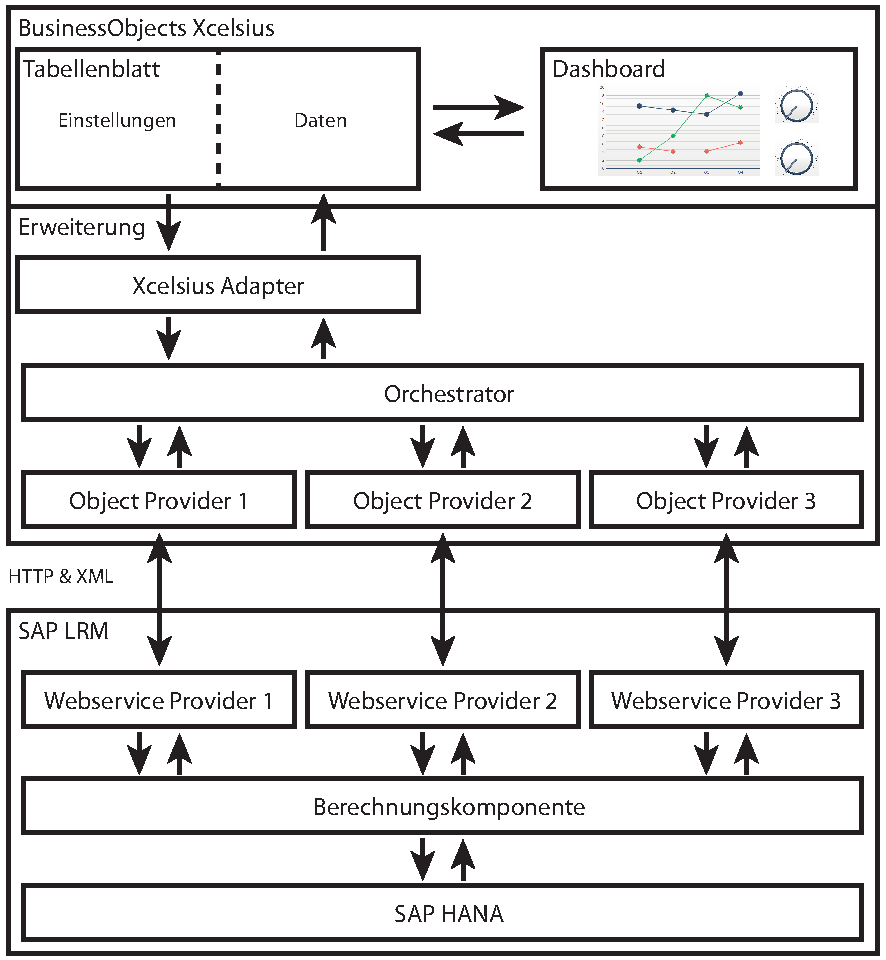
\includegraphics[width=15cm]{images/Abbildung11-Architektur-Erweiterung.pdf}
\caption{Überblick der grundlegenden Architektur der Erweiterung\label{fig:ueberblick-architektur}}
\end{figure}

Im \gls{saplrm} System muss für jeden Webservice ein Webservice-Provider bereitgestellt werden. Der Webservice-Provider kann über einfache Funktionsaufrufe entweder Berechnungen über die Berechnungskomponente durchführen lassen, oder auf Objekte des \gls{saplrm}, wie zum Beispiel einem Laufzeitband oder eine Liquiditätsgruppe, zugreifen. Das Ergebnis liefert er über \gls{http} im \gls{xml}-Format.

Die drei restlichen Teile, die im Überblick eingeführt wurden, werden in einem Plug-in für \gls{xcelsius} implementiert. Dazu zählt die Konsumierung der bereitgestellten Services und anschließend die Orchestrierung.

Der \gls{xcelsius}-Adapter ist über ein Tabellenblatt die Schnittstelle für den Nutzer. Das Tabellenblatt wird dabei in zwei Bereiche unterteilt. Dies sind ein Daten- und ein Ein\-stel\-lungs-Teil. Die Ergebnisse der Erweiterung werden von dem Adapter in den Daten-Teil geschrieben. Damit endet die Zuständigkeit der Erweiterung. Der Nutzer kann die Daten beliebig weiterverarbeiten und zum Beispiel mit Diagrammen visualisieren.

%Blocksatzverletzung
Die Selektionsparameter, die zum Beispiel für die Berechnungskomponente im SAP LRM gebraucht werden (siehe dazu \vref{sec:berechnungskomponente:parameter}), werden aus dem Ein\-stel\-lungs-Teil des Tabellenblatts ausgelesen. Wie die Daten von dem Nutzer in den Bereich geschrieben werden, ist wiederum komplett dem Nutzer überlassen. Eine Möglichkeit sind Kombinationsfelder, die \gls{xcelsius} standardmäßig bereitstellt.

Die Erweiterung stellt nur die Möglichkeit zur Verwendung von Daten aus dem \gls{saplrm} in \gls{xcelsius} bereit. In welcher Form die Daten weiter verarbeitet werden, wird bewusst komplett offengelassen.

\subsection{Statisches Modell}
Für diese Bereiche wurde in einem ersten Schritt die grundlegenden Klassen und ihre Assoziationen zueinander identifiziert. Das entsprechende Klassendiagramm der Analysephase ist in \vref{fig:klassendiagramm_analyse} dargestellt.

\begin{figure}[ht]
\centering
\setlength{\unitlength}{1mm}
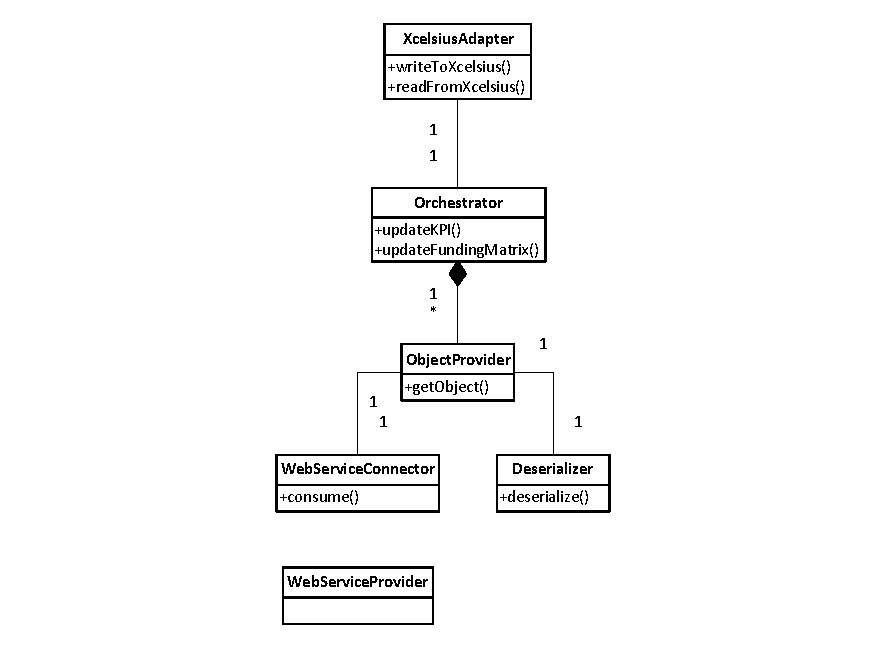
\includegraphics[width=15cm]{Visio/Analyse.pdf}
\caption{Klassendiagramm der Analysephase \label{fig:klassendiagramm_analyse}}
\end{figure}

Das Kernstück der Erweiterung ist die Klasse \class{Orchestrator}. Hier ist die komplette Logik der Orchestrierung für die Kennzahlenanalyse und die Finanzierungsmatrix hinterlegt, das heißt die Ergebnisse der einzelnen Webservices werden kombiniert. Dazu existieren die entsprechenden Methoden \method{updateKPI()} und \method{updateFundingMatrix()}. Für den Datenaustausch mit dem Tabellenblatt von \gls{xcelsius} existiert zwischen der Klasse \class{Orchestrator} und der Klasse \class{XcelsiusAdapter} eine 1:1 Assoziation.

Die Klasse \class{XcelsiusAdapter} stellt die Verbindung zwischen der Erweiterung und dem Tabellenblatt von \gls{xcelsius} dar. Mit der Methode \method{writeToXcelsius()} können Daten in das Tabellenblatt geschrieben werden. Zum Lesen von Daten existiert die Methode \method{readFromXcelsius()}.

Eine weitere wichtige Klasse stellt der \class{ObjectProvider} dar. Ein \class{ObjectProvider} ist eine abstrahierte Schicht über einem Webservice. Die Aufgabe eines \class{ObjectProvider} ist der einfache Zugriff auf Objekte, die über einen Webservice bezogen werden. Dieser Zugriff findet über die Methode \method{getObject()} statt. Mehrere \class{ObjectProvider} sind Teil der Klasse \class{Orchestrator}. Zwischen diesen beiden Klassen existiert eine Komposition.

Um die Webservices abstrahiert darstellen zu können, nutzt ein \class{ObjectProvider} zwei weitere Klassen, den \class{WebServiceConnector} und den \class{Deserializer}. Hier besteht jeweils eine 1:1 Assoziation. Der \class{WebServiceConnector} übernimmt die Kommunikation zwischen der Erweiterung und dem \gls{saplrm} System über \gls{http}. Der \class{Deserializer} wandelt das Resultat der Kommunikation über den Webservice in ein internes Objektformat um.

Die Klasse \class{WebServiceProvider} muss im \gls{saplrm} implementiert werden. Sie nimmt die Anfragen der Erweiterung über \gls{http} entgegen, liest die entsprechenden Objekte aus der Datenbank und serialisiert sie im \gls{xml}-Format.

\subsection{Dynamisches Modell}
Um eine bessere Vorstellung von den Vorgängen zu erlangen, wird in dem Folgenden exemplarisch der Ablauf einer Anfrage durch einen Nutzer erläutert. Das entsprechende Sequenzdiagramm ist in \vref{fig:sequenz_analyse} dargestellt.

\begin{figure}[!ht]
\setlength{\unitlength}{1mm}
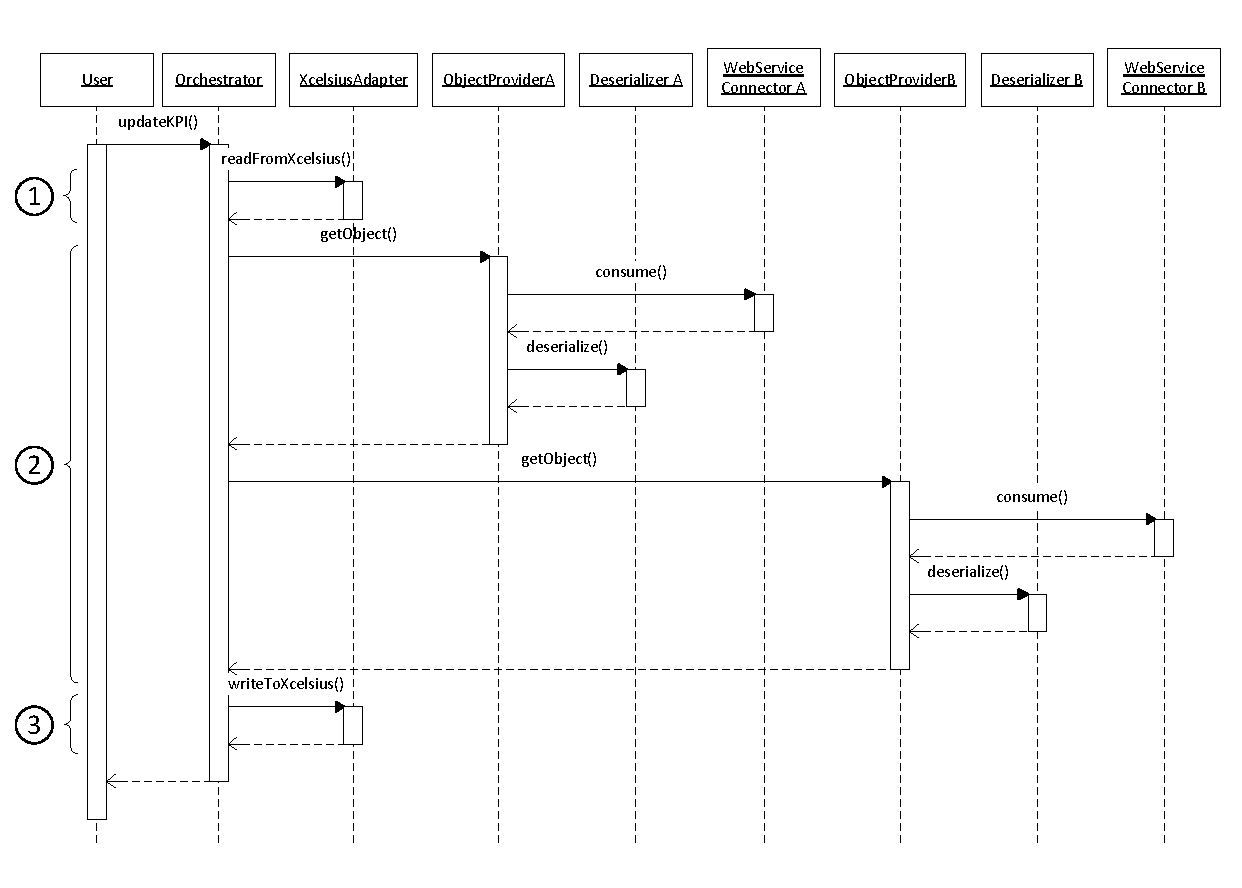
\includegraphics[angle=90,height=197mm]{Visio/Analyse-Sequenz-1.pdf}
\caption{Sequenzdiagramm der Analysephase \label{fig:sequenz_analyse}}
\end{figure} 

In dem Beispiel möchte der Nutzer den Wert einer Kennzahl abfragen. Dazu ruft er in der \instance{Orchestrator}-Instanz die Methode \method{updateKPI()} auf. Daraufhin werden drei Schritte durchlaufen, die in dem Diagramm auf der linken Seite markiert sind. 

Zunächst wird über den \instance{XcelsiusAdapter} die aktuellen Selektionseinstellungen des Nutzers ermittelt. Dazu gehört die Kennzahl, die abgerufen werden soll, und eventuell weitere Einstellungen. Anschließend wird in einem zweiten Schritt ein oder mehrere Webservices über die entsprechenden \instance{WebServiceProvider} konsumiert. Die Objekte, die die \instance{WebServiceProvider} zurückliefern werden durch den \instance{Orchestrator} verbunden.

Die \instance{WebServiceProvider} rufen über einen \instance{WebServiceConnector} den \gls{xml}-Inhalt ab. Anschließend wird das Ergebnis an den entsprechenden \instance{Deserializer} weitergegeben. Dieser wandelt es in eine interne Objektstruktur um und gibt die Instanz an den \instance{ObjectProvider} zurück. Der \instance{ObjectProvider} leitet es an den \instance{Orchestrator} weiter.

Der Aufruf der \instance{WebServiceProvider} durch den \instance{Orchestrator} kann asynchron erfolgen. Hat der \instance{Orchestrator} alle Ergebnisse der \instance{ObjectProvider} erhalten, erfolgt die Umwandlung in das Zielobjektformat und schließlich in dem dritten Schritt das Übergeben des Ergebnisses an den \instance{XcelsiusAdapter}. Dieser schreibt die Daten in das Tabellenblatt von \gls{xcelsius}.

Dadurch stehen die Daten dem Nutzer in \gls{xcelsius} zur Verfügung. Der Aufruf von \method{updateKPI()} ist fertig.

\section{Entwurf}

\subsection{Orchestrierung der Webservices}
Durch die Verwendung eines \gls{glo:abap} Frameworks zur Implementierung von wichtigen Klassen im \gls{saplrm}, existieren schon Webservices, die für die Erweiterungen genutzt werden können. Bei den Klassen handelt es sich um:

\begin{seList}
\item Laufzeitband
\item Liquiditätsszenario
\item Liquiditätsgruppe
\end{seList}

Hierfür bietet das Framework eine Schnittstelle, mit der auf die Objekte über das \gls{glos:atom} zugegriffen werden kann. Diese Webservices können in der Erweiterung genutzt werden. Zusätzlich befindet sich eine iPad-App für das \gls{saplrm} in Entwicklung. Für diese wurden zwei weitere Webservices entwickelt, die dem Zugriff auf Kennzahlen und die Finanzierungsmatrix bieten.

Es ergeben sich fünf nutzbare Webservices, die orchestriert werden müssen. Das Ziel ist immer der Zugriff auf den Webservice der Finanzierungsmatrix oder den Webservice für die Kennzahlen. Die Abhängigkeiten der jeweiligen Webservices sind in \vref{fig:webservice_abhaengigkeiten} dargestellt und sollen im Folgenden erläutert werden:

\begin{figure}[ht]
\centering
\setlength{\unitlength}{1mm}
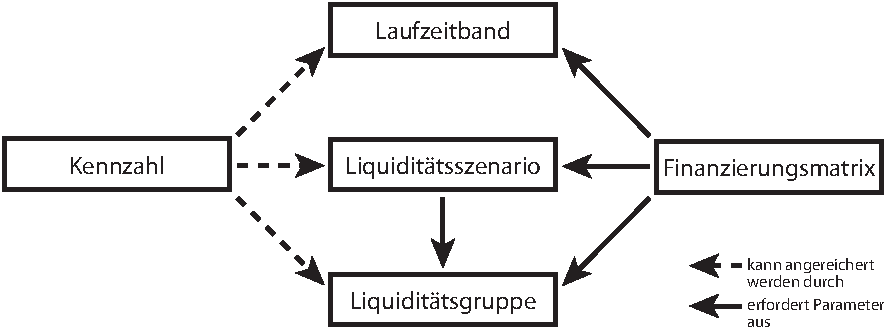
\includegraphics[width=15cm]{images/Abbildung14-Abhaengigkeiten-Webservices.pdf}
\caption{Abhängigkeiten der Webservices\label{fig:webservice_abhaengigkeiten}}
\end{figure}


Der Webservice der Finanzierungsmatrix ruft bei einem Aufruf die Berechnungskomponente des \gls{saplrm} auf und muss demnach mit den vier erforderlichen Parametern versorgt werden (siehe dazu \vref{sec:berechnungskomponente:parameter}). Es besteht eine Abhängigkeit zu den drei Webservices, die automatisch durch das Framework bereit stehen. Der Webservice der Liquiditätsgruppen ist so umgesetzt, dass er ein Liquiditässzenario als Parameter erwartet und darauf alle möglichen Liquiditätsgruppen zurückliefert -- auch hier besteht eine Abhängigkeit.

Der Webservice der Kennzahlen erfordert keine Parameter und kann eigenständig aufgerufen werden. Er liefert alle Kennzahlen, die im \gls{saplrm} angelegt und verfügbar sind. Das Resultat beinhaltet allerdings nicht alle Informationen, zum Beispiel zu dem verwendeten Liquiditätsszenario für die Berechnung oder der dahinter liegenden Liquiditätsgruppe. Das Ergebnis kann also durch weitere Aufrufe von Webservices angereichert werden.

\subsection{Statisches Modell}
Im Gegensatz zu der Analyse wird der Entwurf auf einer höheren Detailstufe durchgeführt und das Resultat der Analyse auch im Hinblick auf die Performance untersucht und optimiert. Das sich daraus ergebende Klassendiagramm ist in \vref{fig:klassendiagramm_entwurf} zu sehen.


\begin{figure}[!ht]
\centering
\setlength{\unitlength}{1mm}
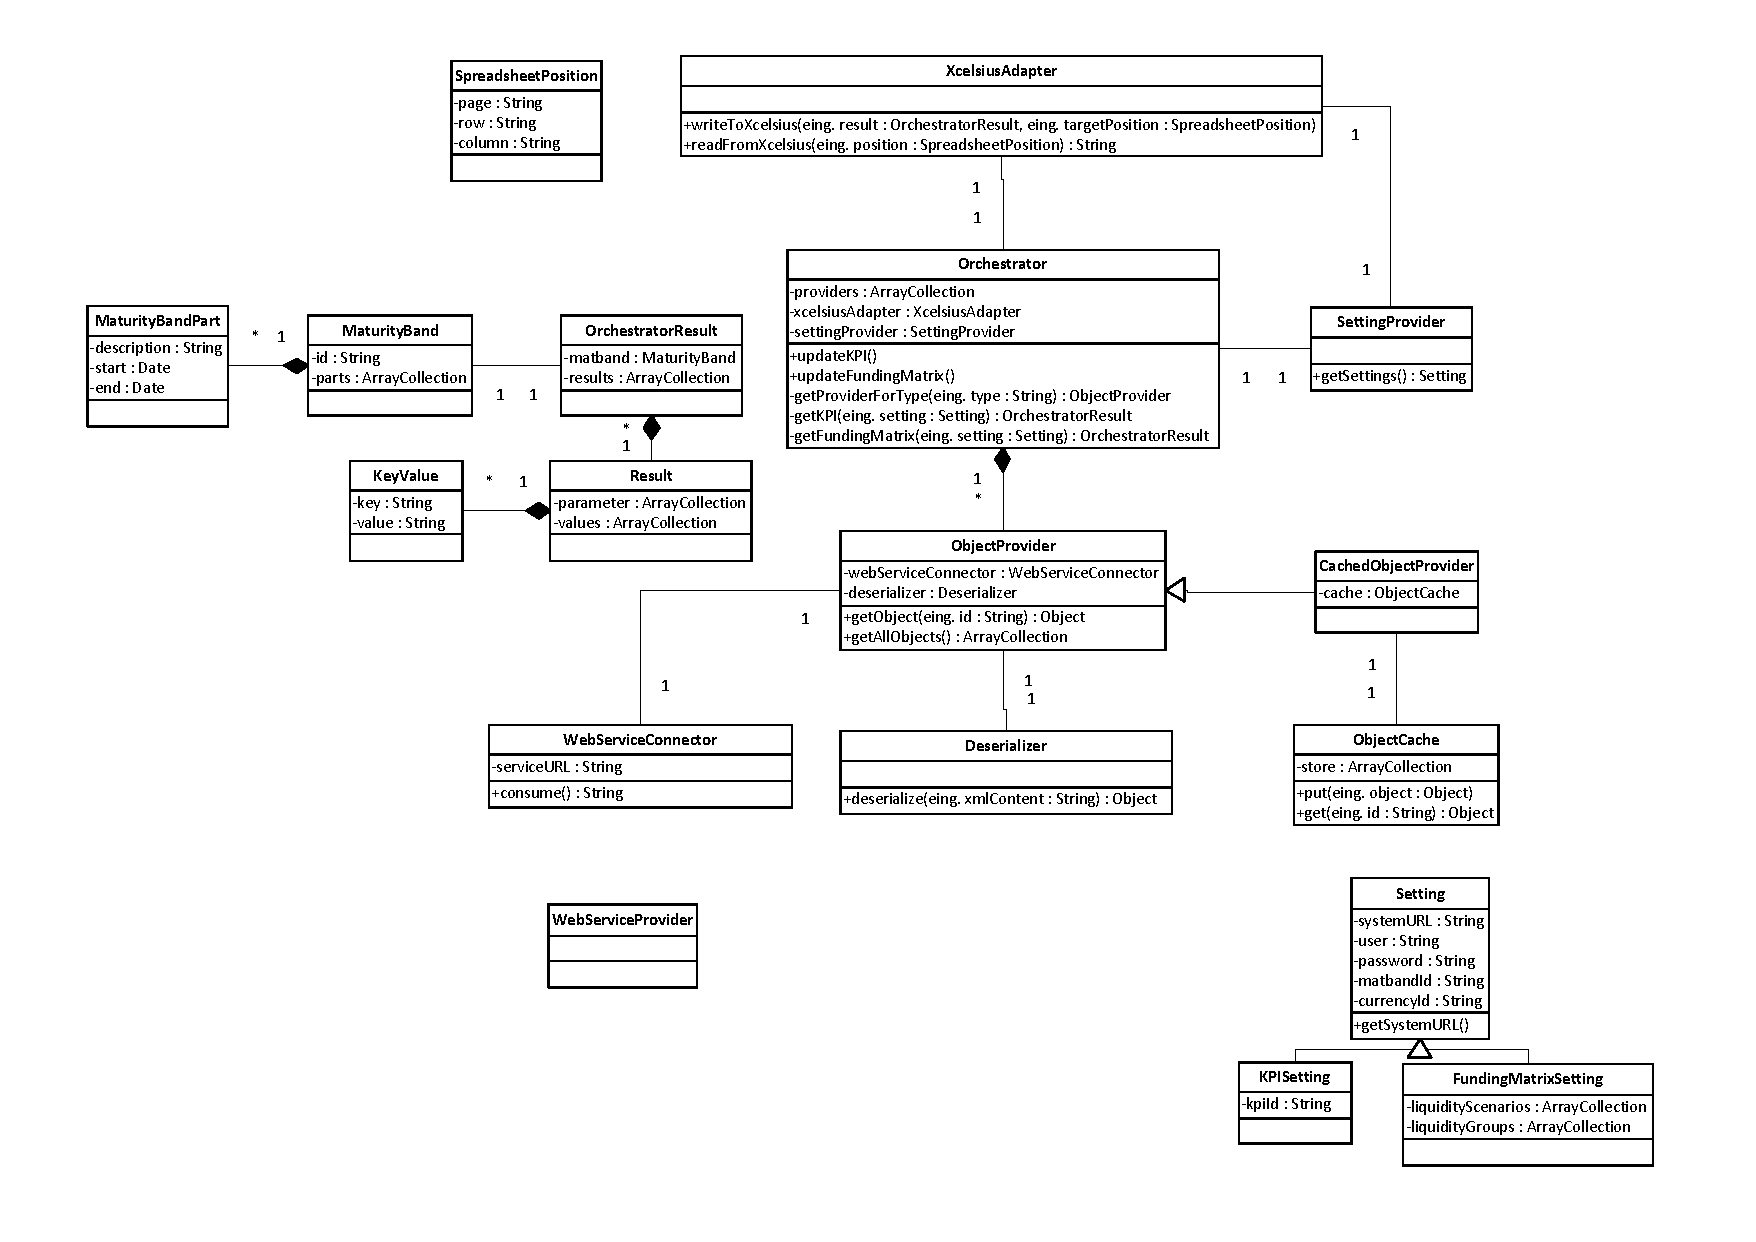
\includegraphics[angle=90,height=197mm]{Visio/Entwurf.pdf}
\caption{Klassendiagramm der Entwurfsphase\label{fig:klassendiagramm_entwurf}}
\end{figure}

Objekte, wie zum Beispiel ein Liquiditätsszenario oder ein Laufzeitband, werden nur einmal angelegt und danach in der Regel nicht mehr geändert. Bei der Orchestrierung der Webservices müsste allerdings nach dem Ergebnis der Analyse jedes Mal eine neue Abfrage gestartet werden. Um das zu verhindern wird die Klasse \class{ObjectProvider} durch die neu hinzugefügte Klasse \class{CachedObjectProvider} erweitert. Ein \class{CachedObjectProvider} hält alle Objekte, die schon einmal angefragt wurden, in einem internen Cache und liefert bei einer erneuten Nachfrage das Objekt aus dem Cache zurück, ohne einen neuen Webservice aufrufen zu müssen.

Für das Ermitteln der aktuellen Einstellungen, die der Nutzer in dem Tabellenblatt von \gls{xcelsius} hinterlegt hat, wurde die Klasse \class{SettingProvider} hinzugefügt. Der \class{SettingProvider} nutzt den \class{XcelsiusAdapter} zum Auslesen des Tabellenblattes und liefert über die Methode \method{getSetting()} alle erforderlichen Einstellungen für die Abfragen der Webservices zurück. Dadurch kann der \class{XcelsiusAdapter} sich rein auf das funktionale Lesen und Schreiben des Tabellenblattes beschränken und von der Logik, welche Zelle in welcher Art ausgelesen werden muss, befreit werden.

Für den einfachen Zugriff auf die einzelnen \class{ObjectProvider} wurde der Klasse \class{Orchestrator} die Hilfsmethode \method{getProviderForType()} hinzugefügt. Die später von dem Nutzer aufgerufenen Methoden \method{updateKPI()} und \method{updateFundingMatrix()} nutzen die neuen Hilfsmethoden \method{getKPI()} und \method{getFundingMatrix()}. Durch die neue Signatur kann der \class{XcelsiusAdapter} und der \class{SettingProvider} einfacher angebunden werden.

\label{sec:entwurf:statisch:orchestratorresult}
Zudem wird mit der Klasse \class{OrchestratorResult} die Zielobjektstruktur der Orchestrierung festgelegt. Eine Instanz der Klasse \class{OrchestratorResult} besteht dabei aus beliebig vielen \class{Result}-Instanzen. Genauer gesagt wird für jede abgefragte Liquiditätsgruppe eine \class{Result}-Instanz erzeugt.

Eine \class{Result}-Instanz hat zum einen mehrere Parameter. Diese sind, um eine gute Erweiterbarkeit zu erreichen, in einfachen Key-Value Paaren verwaltet. Beispiele für Parameter können die Liquiditätsgruppe und das genutzte Liquiditätsszenario sein. Zum anderen werden in dem Attribut \class{values} die einzelnen Werte gespeichert.

Die Werte beziehen sich in ihrer Reihenfolge auf das zugrundeliegende Laufzeitband. Dieses ist für alle \class{Result}-Instanzen das Gleiche und ist deshalb nur einmal als Attribut des \class{OrchestratorResult} vorhanden. Die einzelnen Abschnitte des Laufzeitbandes sind in dem Attribut \class{parts} abgelegt. Ein Laufzeitbandabschnitt hat eine Beschreibung, ein Start- und ein End-Datum.

Generell wurden alle Klassen um typisierte Attribute erweitert. Den Methoden wurde die Signatur hinzugefügt.

\subsection{Dynamisches Modell}

An dem Dynamischen Modell müssen in der Entwurfsphase nur kleinere Änderungen durch die neu hinzugekommenen Klassen durchgeführt werden. Das angepasste Sequenzdiagramm ist in \vref{fig:sequenz_entwurf} dargestellt.

\begin{figure}[!ht]
\centering
\setlength{\unitlength}{1mm}
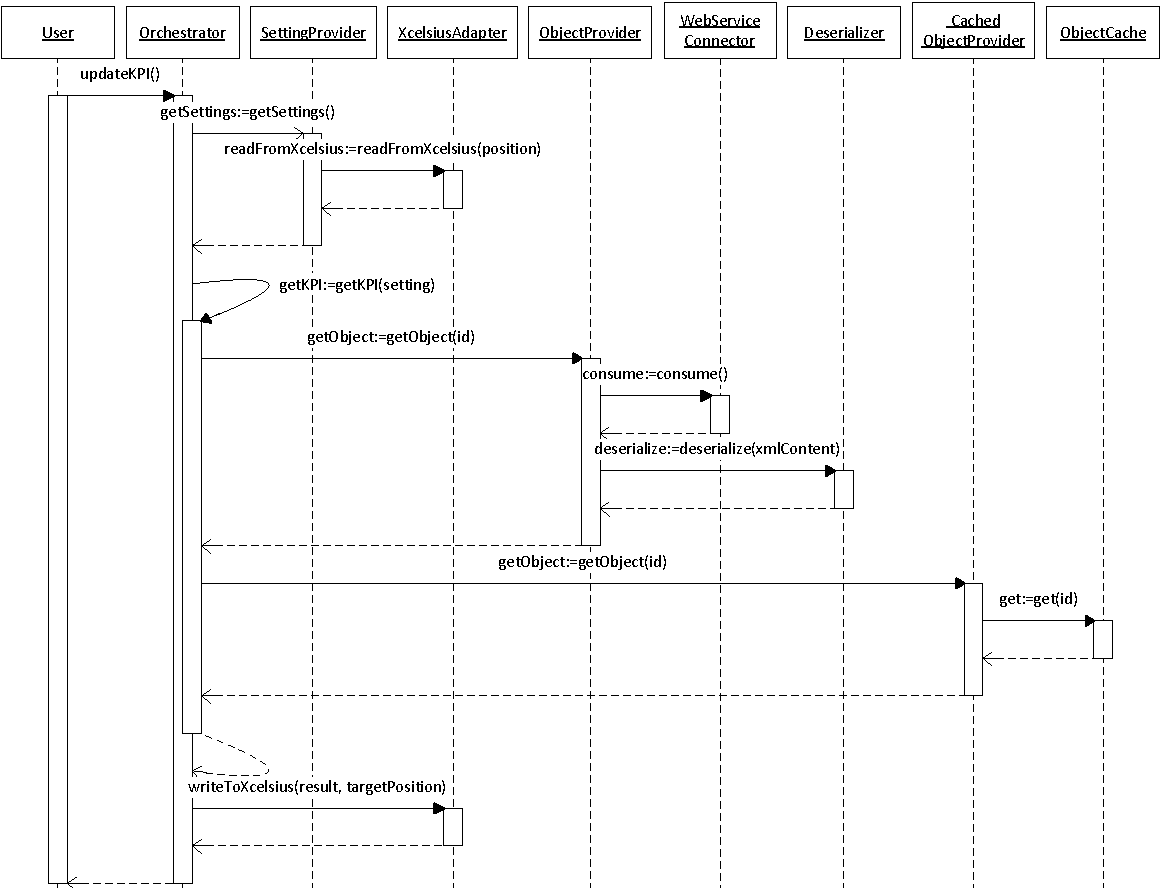
\includegraphics[angle=90,height=197mm]{Visio/Entwurf-Sequenz.pdf}
\caption{Sequenzdiagramm der Entwurfsphase\label{fig:sequenz_entwurf}}
\end{figure}

Am Anfang ist die Einbindung des \class{SettingProvider} zu sehen. Außerdem lässt sich das Zusammenspiel zwischen der öffentlichen, parameterlosen Methode \method{updateKPI()} und der privaten Methode \method{getKPI()} sehen. In der Orchestrierung wird nun auch ein \class{CachedObjectProvider} verwendet. Dieser hatte das angeforderte Objekt schon einmal über seinen Webservice abgefragt und in seinem Cache zwischengespeichert. Dieser Vorgang ist in dem Sequenzdiagramm aus Platzgründen nicht abgebildet. Die erneute Anfrage kann er ohne einen weiteren Aufruf eines Webservices direkt beantworten.

\subsection{Zielstruktur in BusinessObjects Xcelsius}
Eine zentrale Rolle in der Erweiterung spielt die Übergabe der Ergebnisse der Orchestrierung an das Tabellenblatt von \gls{xcelsius}. Dies muss in einer Art und Weise geschehen, sodass der Nutzer die Daten später einfach weiterverarbeiten oder visualisieren kann.

Diese Aufgabe wird von dem \class{XcelsiusAdapter} übernommen. Ausgangspunkt ist immer eine \class{OrchestratorResult}-Instanz, welche das Ergebnis der Orchestrierung darstellt. Den Aufbau der Instanz ist in \vref{sec:entwurf:statisch:orchestratorresult} dargestellt. Diese Objektstruktur muss in eine Tabellenstruktur in \gls{xcelsius} umgewandelt werden. Ein konkretes Beispiel für die Objektstruktur zeigt \vref{fig:objektstruktur}, welches in \vref{tab:zielstruktur} entsprechend umgesetzt ist.

\begin{figure}[ht]
\centering
\setlength{\unitlength}{1mm}
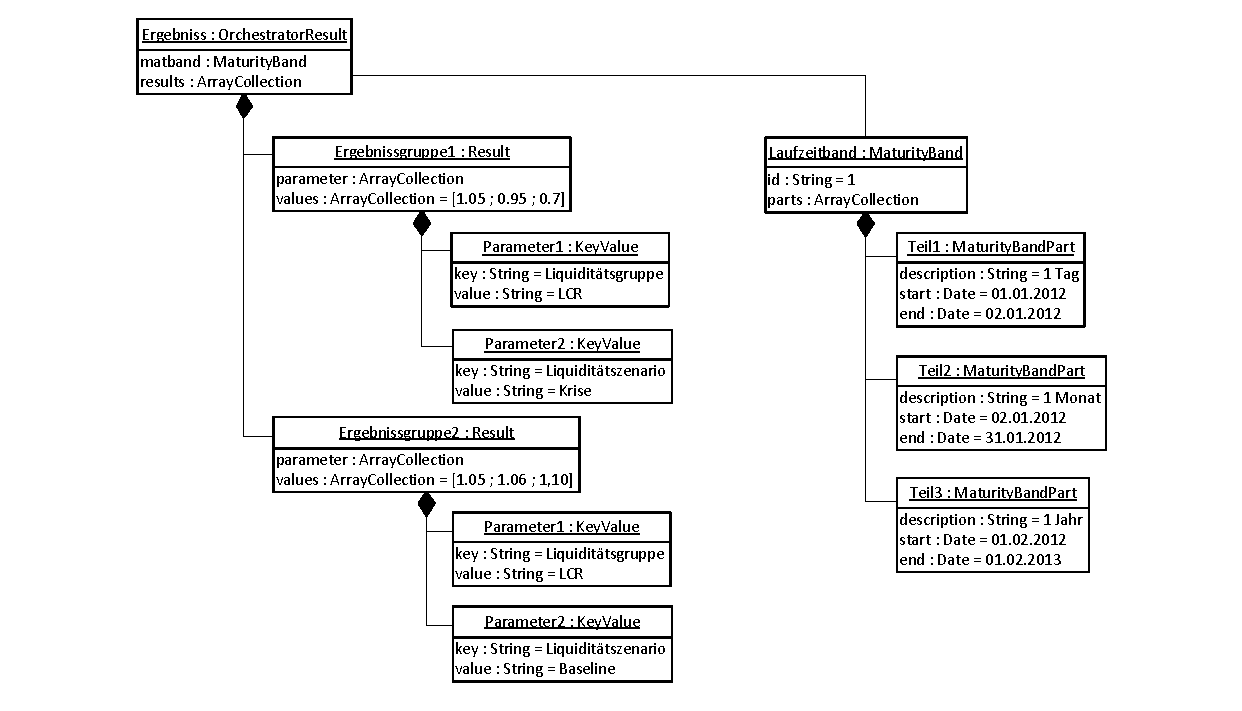
\includegraphics[width=15cm]{Visio/Entwurf-Objektstruktur.pdf}
\caption{Interne Objektstruktur vor der Umwandlung durch den Xcel\-si\-us\-Adap\-ter \label{fig:objektstruktur}}
\end{figure} 

% Table generated by Excel2LaTeX from sheet 'Sheet1'
\begin{table}[ht]
  \centering
  \caption{Ergebnis der Umwandlung durch den XcelsiusAdapter}
    \begin{tabular}{l|r|r}
    \toprule
    \textbf{Liquiditätsgruppe:} & \textbf{FLE} & \textbf{FLE} \\
    \textbf{Liquiditätsszenario:} & \textbf{Krise} & \textbf{Baseline} \\
    \midrule
    1 Tag & 1,05  & 1,05 \\
    1 Monat & 0,95  & 1,06 \\
    1 Jahr & 0,70  & 1,10 \\
    \bottomrule
    \end{tabular}%
  \label{tab:zielstruktur}%
\end{table}%

Die Tabellenstruktur soll folgendermaßen aufgebaut werden: Eine Ergebnisreihe wird immer in einer Spalte dargestellt. Dabei handelt es sich um alle Ergebniswerte, die für eine Liquiditätsgruppe ermittelt wurden. Die Ergebnisreihen sind in der Objektstruktur die \class{Ergebnis}-Instanzen. Die Werte sind in der ArrayCollection \class{values} gespeichert. Sie beziehen sich auf die einzelnen Abschnitte des zugrundeliegenden Laufzeitbandes.

In der ersten Spalte werden die Abschnitte des Laufzeitbandes abgetragen. Diese können zum Beispiel später in einer Visualisierung als X-Achsenbeschriftung verwendet werden. In der Objektstruktur sind das die \instance{Laufzeitbandabschnitt}-Instanzen. In einer Zeile in der Tabellenstruktur sind demnach die Werte aller \class{Ergebnis}-Instanzen für ein Laufzeitbandabschnitt eingetragen.

Über den eigentlichen Werten werden noch die Parameter eingetragen, die als Key-Value-Paar in der \class{Ergebnis}-Instanz vorhanden sind. Sie können bei einer Visualisierung als Beschriftung für eine Ergebnisreihe verwendet werden.

So entsteht die Tabellenstruktur in \vref{tab:zielstruktur}, welche durch den \class{XcelsiusAdapter} in das Tabellenblatt geschrieben wird. Dort können die Daten durch den Nutzer weiterverarbeitet werden.

\section{Implementierung}
\subsection{Adobe Flex Sandbox}
Alle Anwendungen, die mit Hilfe von Adobe Flex programmiert sind, unterliegen bestimmten Sicherheitsbeschränkungen. Darunter fällt auch die Erweiterung, die im Rahmen dieser Bachelorarbeit entwickelt wird. Die Ausführung von Adobe Flex-Anwendungen erfolgt in einer Sandbox. Dadurch sollen ungewollte Änderungen auf Client-Seite verhindert werden. Die Anwendung darf sich nur in einem klar definierten Raum bewegen.

Eine dieser Beschränkungen ist die Verhinderung von Cross-Domain Requests. Dabei handelt es sich um einen Aufruf eines Webservices, dessen Ziel eine andere Domain ist. In dem konkreten Beispiel der Erweiterung für \gls{xcelsius} ist die Domain der lokale Computer (localhost). Es ist nur möglich, Webservices aufzurufen, die der Computer selbst bereitstellt. Das \gls{saplrm} selbst läuft nicht auf dem Computer, sondern auf einem Server in einer eigenen Domain. Dadurch ist das Konsumieren von Daten aus dem \gls{saplrm} zunächst nicht möglich, da es durch die Sandbox blockiert wird. Die Beschränkung ist in \vref{fig:flex_sandbox} dargestellt.

\begin{figure}[ht]
\centering
\setlength{\unitlength}{1mm}
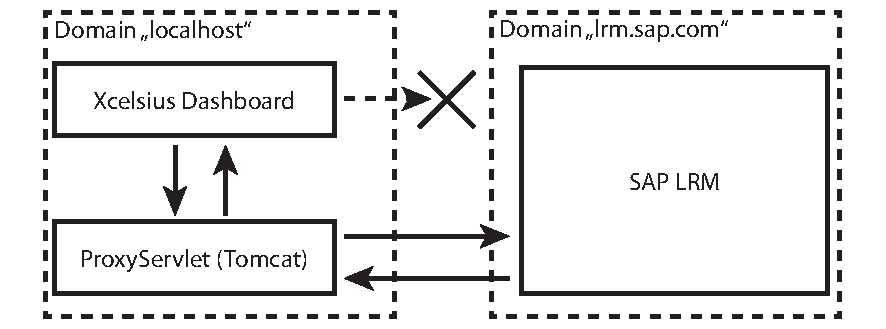
\includegraphics[width=15cm]{images/Abbildung18-Flex-Sandbox.pdf}
\caption{Sandbox-Problematik von Adobe Flex\label{fig:flex_sandbox}}
\end{figure}

Für dieses Problem kommen zwei Lösungsansätze in Frage. Zum einen ist es möglich, dass der Anbieter des Webservices explizit festlegen kann, dass der Webservice auch über verschiedene Domains hinweg konsumiert werden kann. Dies geschieht über eine Datei crossdomain.xml, welche in dem Hauptverzeichnis der Domain abgelegt werden muss. Bei der Erweiterung wäre das der Anwendungsserver des \gls{saplrm}. Änderungen an diesem zu veranlassen würde einen hohen Aufwand benötigen. 

Um diesen Aufwand zu umgehen, wurde der zweite Lösungsansatz umgesetzt. Hierbei wird auf dem Client ein lokaler Webserver installiert. Dieser Webserver ist über die Domain localhost erreichbar. Alle Anfragen der Erweiterung gehen gegen den lokalen Webserver. Dadurch, dass die Adobe Flex-Anwendung auch unter der Domain localhost ausgeführt wird, ist der Zugriff erlaubt. Der Webserver stellt die Anfrage an den richtigen Webservice im \gls{saplrm} und leitet die Antwort an die Erweiterung weiter.

Für die Umsetzung wurde lokal ein \gls{glos:tomcat}-Webserver installiert. Für diesen wurde ein einfaches Java-HttpServlet entwickelt, welches die geforderte Funktionalität umsetzt. Der Quelltext des Servlets ist in \vref{listing:servlet} zu sehen.

Für die Zukunft sollte allerdings versucht werden, die Lösung über die Datei crossdomain.xml umzusetzen. Dadurch entfällt der zusätzlich notwendige lokale Webserver.

\subsection{Asynchroner Programmablauf}
\label{sec:asynchron}
Im Vergleich zu dem Entwurf und der Analyse, bei dem alle Aufrufe synchron durchgeführt wurden, wird dies aus zwei Gründen in der Umsetzung auf hauptsächlich asynchrone Aufrufe umgestellt. Dabei handelt es sich um folgende Gründe:

Auf der einen Seite kann sich dadurch ein Geschwindigkeitsvorteil ergeben. Falls sich bei der Orchestrierung die Antwort eines Webservice-Aufrufes verzögert, können trotzdem alle anderen Anfragen schon verarbeitet werden. Der dadurch gewonnene Vorteil ist aufgrund einer Limitierung durch das verwendete Framework jedoch nicht sehr groß, da die Anwendung später nur auf einem Thread ausgeführt wird. Eine echt-parallele Verarbeitung von zwei simultan erhaltenen Antworten ist somit nicht möglich.

Auf der anderen Seite wird für den Aufruf der Webservices in der Klasse \class{WebServiceConnector} die Adobe Flex-Klasse \class{HTTPService} verwendet. Diese bietet nur die Möglichkeit über \class{EventListener} auf zwei Events, nämlich dem erfolgreichen Aufruf des Webservices und dem fehlgeschlagen Aufruf zu reagieren. Dabei werden zwei Callback-Methoden angegeben, die dann asynchron aufgerufen werden. Ab diesem Zeitpunkt endet somit der bis dahin ausschließlich synchrone Aufruf. Der entsprechende Quelltext ist in \vref{listing:ws_aufruf} dargestellt.

\begin{programm}[ht]
\begin{lstlisting}[language=ActionScript]
public function consume():void{
	// HTTPService-Instanz erstellen
	webService = new HTTPService();
	webService.url = serviceURL;     
	webService.method = "GET";
	// Event Listener hinzufuegen
	webService.addEventListener(ResultEvent.RESULT,onHttpRequestSuccess);
	webService.addEventListener(FaultEvent.FAULT,onHttpRequestFailure);
	// Anfrage senden
	webService.send();
}
		
public function onHttpRequestSuccess(event:ResultEvent):void{
	// Asynchroner Aufruf bei Erfolg
	// ...
}
		
public function onHttpRequestFailure(event:FaultEvent):void{
	//Asynchroner Aufruf bei Fehlschlag
	// ...
}
\end{lstlisting}
\caption{Aufruf eines Webservices in der Erweiterung\label{listing:ws_aufruf}}
\end{programm}

Durch die Asynchronität ändert sich entsprechend die Signatur der Methoden. Der Rückgabewert entfällt, stattdessen wird ein zusätzlicher Parameter mitgegeben. Bei \gls{glos:actionscript} kann dies entweder eine Methode eines Objektes sein, siehe dazu \vref{listing:ws_aufruf}. Alternativ kann auch eine Objekt-Instanz übergeben werden. Auf dieser Instanz wird dann zu dem entsprechenden Zeitpunkt eine festgelegte Methode aufgerufen.

Anfang und Ende eines Aufrufes von einem Webservice über den \class{ObjectProvider} und den \class{Deserializer} ist der \class{Orchestrator}. Dieser startet die Aufrufe in der Methode \method{getKPI()} oder \method{getFundingMatrix()} und erhält die Antworten durch die Asynchronität in beliebiger Reihenfolge in der Methode \method{onObjectProviderSuccess()}. Um die Aufrufe unterscheiden und identifizieren zu können, wird bei dem Aufruf ein \class{RequestToken} mitgegeben. Dieser wird weitergereicht und schließlich auch der Methode \method{onObjectProviderSuccess()} als Parameter zurückgegeben.

Um festzustellen, ob alle Anfragen erfolgreich zurückgekommen sind und somit mit der finalen Orchestrierung begonnen werden kann, werden die \class{RequestToken} in einer internen Liste verwaltet. Diese Liste enthält alle Anfragen, von denen die Antwort noch aussteht. Wird die Antwort erhalten, wird der Token aus der Liste entfernt, in einen \class{ResultToken} umgewandelt, indem das eigentliche Ergebnis angehängt wird, und in einer weiteren Liste zwischengespeichert. Wurden alle Anfragen erfolgreich beantwortet, kann die Orchestrierung durchgeführt werden. Die einzelnen Ergebnisse können dann aus der Liste mit den \class{ResultToken}-Instanzen bezogen werden.

Die Methode \method{onObjectProviderSuccess()} wird asynchron aufgerufen und verändert unter anderem die beiden Listen zur Verwaltung der Token. Demnach handelt es sich hierbei normalerweise um einen kritischen Abschnitt, in dem kritische Daten verändert werden. Der Zugriff auf diese Methode müsste synchronisiert werden. Da aber die Anwendung später auf nur einem Thread ausgeführt wird, kann auf eine Synchronisation verzichtet werden.

In \vref{listing:orchestrierung:webservices} ist in allgemeiner Form der erläuterte Ablauf implementiert. Dabei werden zwei beliebige \class{ObjectProvider} abgefragt. Die jeweiligen Ergebnisse können dann in gewünschter Weise orchestriert werden. Die in dem Beispiel verwendeten Klassen wurden teilweise vereinfacht und entsprechen nicht den Klassen in dem statischen Modell der Erweiterung.

\begin{programm}[ht]
\begin{lstlisting}[language=ActionScript]
private function orchestrateWebServices():void{
	// Verwaltung der Token
	pendingRequestToken = new ArrayCollection();
	finishedRequestToken = new ArrayCollection();
	
	// Beispielhafte Anfrage an ein ObjectProvider
	var objectProviderA:ObjectProvider = new ObjectProvider();
	var token:RequestToken = new RequestToken(RequestToken.REQUEST_A);
	pendingRequestToken.addItem(token);
	objectProvider.getObject(token,this);
	
	// beliebige weitere Anfragen an ObjectProvider ...
}
// Callback-Methode fuer die ObjectProvider
public function onObjectProviderSuccess(result:Object, token:RequestToken):void{
	// Ergebnis der Anfrage vermerken
	pendingRequestToken.removeItemAt(pendingRequestToken.getItemIndex(token));
	finishedRequestToken.addItem(new ResultToken(token,result));
	
	if(pendingRequestToken.length == 0){ // alle Ergebnisse liegen vor
		// Zugriff auf Ergebnisse
		var ergA:Object = getResultForRequest(RequestToken.REQUEST_A);
		// Ergebnisse orchestrieren ...
	}
}
// Hilfsmethode fuer den Zugriff auf ein Resultat	
private function getResultForRequest(request:String):Object{
	for each(var token:ResultToken in finishedRequestToken){
		if(token.attribute == request)
			return token.result;
	}
	throw "no result";
}
\end{lstlisting}
\caption{Beispielhafter Ablauf der Orchestrierung von Webservices\label{listing:orchestrierung:webservices}}
\end{programm}


\subsection{Webservice-Ablauf}
In diesem Abschnitt soll an dem Beispiel des Finanzierungsmatrix-Webservices exemplarisch gezeigt werden, wie der Aufruf und die Umwandlung in ein internes Objektformat realisiert wird.

Der Ausgangspunkt ist dazu der \class{Orchestrator}, der die \method{getObject()}-Methode des \class{FundingMatrixObjectProviders} aufruft. Zunächst wird hier die passende \gls{url} für den Webservice-Aufruf auf Grundlage der Einstellungen generiert. In diesem Fall werden über die \gls{url} die Parameter Liquiditätsgruppen, Liquiditätsszenarien, Laufzeitband und Zielwährung übergeben. Es wird eine \class{WebserviceConnector}-Instanz erzeugt und über die \method{consume()}-Methode des \class{WebserviceConnectors} der eigentliche Aufruf gestartet. Entsprechend dem asynchronen Programmablauf, siehe dazu \vref{sec:asynchron}, wird die eigene Instanz als Callback und der \class{RequestToken} mitgegeben.

Tritt bei dem Aufruf ein Fehler auf, wird asynchron die Methode \method{onWebServiceFail()} aufgerufen. Der Fehler muss nur dem \class{Orchestrator} weitergeleitet werden. Dazu wurde auch hier bei dem \method{getObject()}-Aufruf eine Referenz auf den \class{Orchestrator} als Callback mitgegeben.

Wenn kein Fehler auftritt, wird statt der Methode zur Behandlung des Fehlers die \method{onWebServiceSuccess()}-Methode aufgerufen. Der Parameter \class{ResultEvent} enthält die Antwort des Webservices als Zeichenkette. Diese muss nun in die interne Objektstruktur umgewandelt werden. Dazu wird der \class{FundingMatrixObjectDeserializer} verwendet. Die \gls{xml}-Eingabe für den \class{Deserializer} und die daraus generierte Objektstruktur ist in \vref{fig:umwandlung:ueberblick} dargestellt.

\begin{figure}[ht]
\centering
\setlength{\unitlength}{1mm}
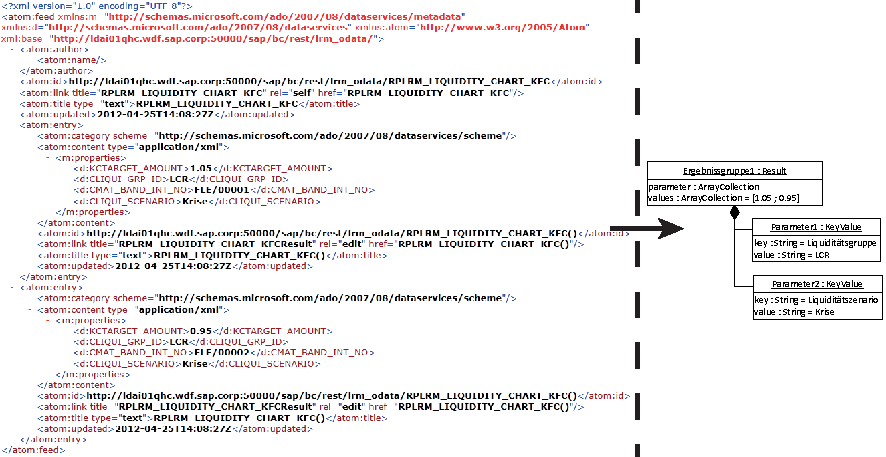
\includegraphics[width=15cm]{images/Abbildung21-Umwandlung.pdf}
\caption{Umwandlung der XML-Antwort in die interne Objektstruktur\label{fig:umwandlung:ueberblick}}
\end{figure}

Bei der Deserialisierung kann wiederum auf Hilfsklassen von Adobe Flex zugegriffen werden. Über die Klasse \class{SimpleXMLDecoder} kann einfach ein Proxy-Objekt erzeugt werden. Dadurch kann auf die einzelnen Elemente in der \gls{xml}-Struktur wie auf Attribute eines Objektes zugegriffen werden. Der Quellcode der Umwandlung, wie sie in \vref{fig:umwandlung:ueberblick} dargestellt ist, findet sich in \vref{listing:deserialisierung}.


\begin{programm}[ht]
\begin{lstlisting}[language=ActionScript]
public override function deserialize(content:String):Object{			
	var decoder:SimpleXMLDecoder = new SimpleXMLDecoder();
	var proxyObject:Object = decoder.decodeXML(new XMLDocument(content));
	
	var result:ArrayCollection = new ArrayCollection();
	var resultGroup:Result = null;			
			
	for each(var entry:Object in proxyObject.feed.entry as Array){
		var liquiGroup:String = entry.content.properties.CLIQUI_GRP_ID as String;
		var liquiScenario:String = entry.content.properties.CLIQUI_SCENARIO as String;
		if(resultGroup == null || resultGroup.getParameter(Result.LIQUIDITY_GROUP) != liquiGroup || resultGroup.getParameter(Result.LIQUIDITY_SCENARIO) != liquiScenario){
			if(resultGroup != null) // dont add null at first time
				result.addItem(resultGroup);
			resultGroup = new Result();
			resultGroup.addParameter(new KeyValue(Result.LIQUIDITY_GROUP,liquiGroup));
			resultGroup.addParameter(new KeyValue(Result.LIQUIDITY_SCENARIO,liquiScenario));
		}
		var value:Number = entry.content.properties.KCTARGET_AMOUNT as Number;
		resultGroup.addValue(value);
	}
	result.addItem(resultGroup);
	return result;
}
\end{lstlisting}
\caption{Deserialisierung des XML-Formats in die interne Objektstruktur\label{listing:deserialisierung}}
\end{programm}


Die \class{ObjectProvider} und \class{Deserializer} für die weiteren Webservices sind analog dazu programmiert. Bei einem \class{CachedObjectProvider} wird in der \method{getObject()}-Methode zunächst ermittelt, ob sich das angeforderte Objekt schon im Cache befindet und dann direkt zurückgegeben. Ist es noch nicht vorhanden, wird der Webservice-Aufruf gestartet und nach der Deserialisierung wird das Objekt im Cache für weitere Anfragen gehalten.

\subsection{BusinessObjects Xcelsius Binding}
\label{sec:xcelsius_binding}
Für den Datenaustausch zwischen der entwickelten Erweiterung und dem Tabellenblatt von \gls{xcelsius} muss auf die bereitgestellten Funktionen des \gls{xcelsius} \gls{glos:sdk} zurückgegriffen werden. Dabei wird das Konzept des Bindings genutzt.

Bei diesem Konzept wird ein Attribut einer Instanz fest mit einem Zellenbereich auf dem Tabellenblatt verbunden. Dabei kann es sich entweder um ein flaches Attribut, wie zum Beispiel eine Zeichenkette oder eine Zahl, handeln, die dann mit einer einzelnen Zelle auf dem Tabellenblatt verbunden wird. Es kann allerdings auch auf einer Tabellenblatt-Seite ein Bereich festgelegt werden, der dann zum Beispiel mit einem zweidimensionalen Array verbunden wird.

Für solch eine Verbindung muss zusätzlich noch eine Richtung festgelegt werden. Das \gls{xcelsius} \gls{glos:sdk} bietet dabei drei Möglichkeiten an:

\begin{seToplist}{ XXX }

\item[1.] \textbf{Input-Binding} \newline
Bei einem Input-Binding findet der Datenfluss nur von dem Tabellenblatt zu der Erweiterung statt. Er dient damit ausschließlich dazu, auf das Tabellenblatt lesend zuzugreifen. Sobald sich der Wert im Tabellenblatt ändert, wird diese Änderung auf das Attribut übertragen.

\item[2.] \textbf{Output-Binding} \newline
Das Output-Binding bietet ausschließlich schreibenden Zugriff auf das Tabellenblatt. Wird also der Attributswert verändert, wird die dazugehörige Zelle oder der Zellenbereich entsprechend angepasst. Der Datenfluss findet nur von der Erweiterung zu dem Tabellenblatt statt.

\item[3.] \textbf{Input-Output-Binding} \newline
Bei dieser Verbindungsart findet zwischen dem Tabellenblatt ein beidseitiger Austausch statt. Von beiden Seiten her werden Veränderungen auf die jeweils andere Seite übertragen. Der Wert der Zelle wird mit dem Attributswert synchronisiert.

\end{seToplist}

Für die Umsetzung der Erweiterung spielen Input-Output-Bindings keine Rolle. Es werden nur Input- oder Output-Bindings verwendet. Das Auslesen der gewählten Parameter findet über mehrere Input-Bindings statt. Für das Laufzeitband wird dabei eine Zelle mit dem Attribut \class{selectedMaturityBand} des \class{XcelsiusAdapter} verknüpft. Bei den Liquiditätsszenarien und den Liquiditätsgruppen können jeweils mehrere ausgewählt werden. Hier bezieht sich das Binding demnach nicht auf eine einzelne Zelle, sondern auf einen Zellenbereich.

Neben der Berechnung der Finanzierungsmatrix und der Einbindung der Kennzahlenanalyse wird unterstützend eine Wertehilfe angeboten. Auch dafür müssen entsprechende Bindings angelegt werden. Die Wertehilfe bietet zum einen alle im \gls{saplrm} vorhandenen Liquiditätsszenarien an. Diese können dann als Grundlage für Kombinationsfelder genutzt werden.

Neben der Wertehilfe für die Liquiditätsszenarien existiert eine weitere Wertehilfe für Liquiditätsgruppen. Diese basiert auf den aktuell ausgewählten Liquiditätsszenarien und liefert für diese die existierenden Liquiditätsgruppen zurück.

Eine letzte Wertehilfe wurde für die Laufzeitbänder hinzugefügt. Durch diese Wertehilfen ist es für den Nutzer später einfacher, gültige Selektionskriterien festzulegen. Der Nutzer muss nicht den Namen der existierenden Gruppen, Szenarien oder Laufzeitbänder kennen, er braucht sie nur aus einer Liste auszuwählen.

\section{Zusammenfassung}
In diesem Kapitel wurde der komplette Entwicklungsprozess, bestehend aus der Analyse, dem Entwurf und der Implementierung, dargelegt. Das Ergebnis ist eine Erweiterung für \gls{xcelsius}, mit der \gls{xcelsius} zur Visualisierung der Daten des \gls{saplrm} genutzt werden kann. Dabei werden die Vorteile der Berechnungskomponente des \gls{saplrm} und die Geschwindigkeit von SAP HANA ausgenutzt. Gleichzeitig ist durch die modulare Struktur der Grundstein für zum einen Weiterentwicklungen des \gls{saplrm} als auch die Integration des \gls{saplrm} mit weiteren Anwendungen gelegt. Die Evaluierung der Ergebnisse wird in dem folgenden Kapitel durchgeführt.

\chapter{Evaluation der Erweiterung für BusinessObjects Xcelsius}

\section{Einleitung}
In diesem Kapitel wird die Evaluation der im Rahmen der Bachelorarbeit entwickelten Erweiterung durchgeführt. Dabei wird die Erweiterung insbesondere auf zwei Aspekte hin genauer untersucht. Zum einen soll aufgezeigt werden, welche neuen Möglichkeiten sich mit der Erweiterung ergeben und wie diese genutzt werden können. Außerdem muss überprüft werden, in wiefern die Anforderungen und die Zielsetzung, die in der Spezifikation in \vref{sec:spezifikation} festgelegt wurden, erfüllt werden können.

\section{Neue Möglichkeiten}
Durch die Erweiterung ist es nun möglich, \gls{xcelsius} in Verbindung mit den Daten des \gls{saplrm} zu nutzen. Dazu muss zu einem Dashboard lediglich eine neue Verbindung, die Teil der Erweiterung ist, hinzugefügt werden.

Für diese Verbindung müssen in den Einstellungen dann einige erforderliche Bindings, siehe dazu \vref{sec:xcelsius_binding}, festgelegt werden. Der Dialog zum Festlegen der Einstellungen ist in \vref{fig:einstellung} zu sehen. Erforderlich sind hierbei der Nutzer mit entsprechendem Passwort für die Authentifizierung, und die \gls{url}, unter der das \gls{saplrm} erreichbar ist.

\begin{figure}[ht]
\centering
\setlength{\unitlength}{1mm}
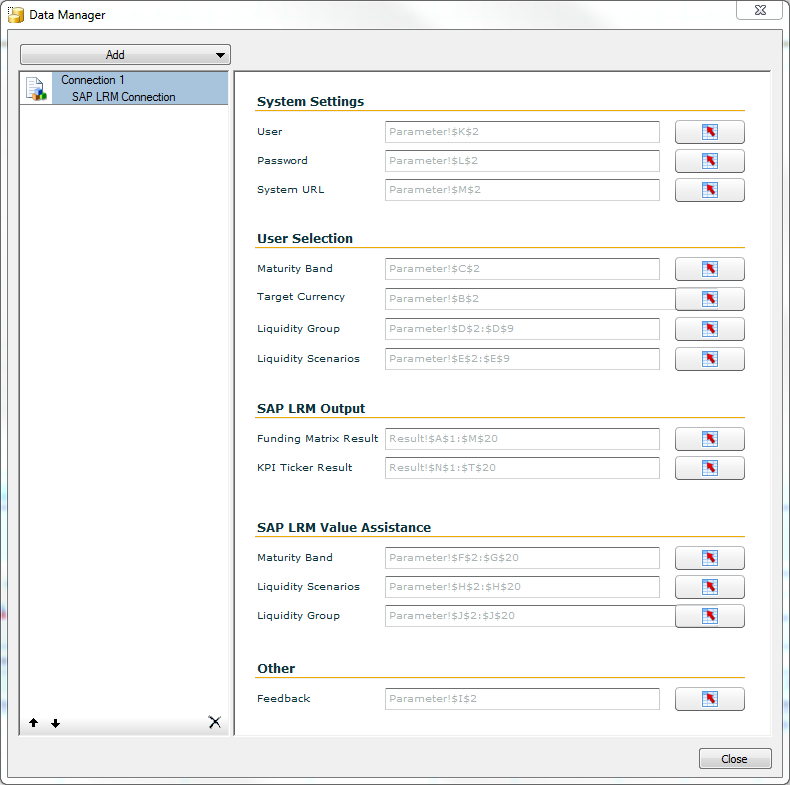
\includegraphics[width=10cm]{images/xcelsius_einstellungen.PNG}
\caption{Einstellungsmöglichkeiten der Erweiterung für BusinessObjects Xcelsius\label{fig:einstellung}}
\end{figure} 

Für die Finanzierungsmatrix müssen für alle erforderlichen Parameter für die Berechnungskomponente (vgl. \vref{sec:berechnungskomponente:parameter}) und ein Bereich, in den das Ergebnis geschrieben wird, mit Bindings verbunden werden.

Da die Kennzahlenanalyse keine Parameter erfordert, reicht hier ein Binding für das Ergebnis. Die Wertehilfen, die zusätzlich angeboten werden, können genutzt werden, sind aber nicht zwingend erforderlich. Wenn der Nutzer sich dafür entscheidet, sie anzuwenden, muss entsprechend für jede Hilfe auch ein Binding erzeugt werden.

In dem erstellten Beispieldashboard wurden alle zur Verfügung stehenden Funktionalitäten ausgenutzt. Die Finanzierungsmatrix wurde als Liniendiagramm dargestellt. Die erforderlichen Parameter werden durch die Kombinationsfelder auf der linken Seite festgelegt. Die Auswahlmöglichkeiten beruhen dabei auf der angebotenen Wertehilfe. 

An dieser Stelle wären durchaus auch noch andere Möglichkeiten denkbar, zum Beispiel über Checkboxen oder ähnlichen Auswahlelementen. Dies zeigt, dass die Erweiterung hier keinerlei Beschränkungen vorgibt. Die Form des Parameter-Inputs und der Verarbeitung der Ergebnisse ist komplett offen gehalten und nur durch die Möglichkeiten von \gls{xcelsius} beschränkt.

Die Kennzahlenanalyse, die in der ursprünglichen Situation, wie in \vref{fig:lrm_istzustand_keyfigureanalysis} zu sehen, nur als einfache Tabelle dargestellt wurde, kann nun beliebig visualisiert werden. In dem Beispiel zeigt sich dies durch die Tachometer.


\section{Erfüllung der Anforderungen}
An die Erweiterung wurden in der Spezifikation in \vref{sec:anforderungen} einige funktionale und nicht-funktionale Anforderungen gestellt. Um diese zu überprüfen wurde ein Beispieldashboard, das in \vref{fig:umsetzung_dashboard} zu sehen ist, erstellt.

\begin{figure}[ht]
\centering
\setlength{\unitlength}{1mm}
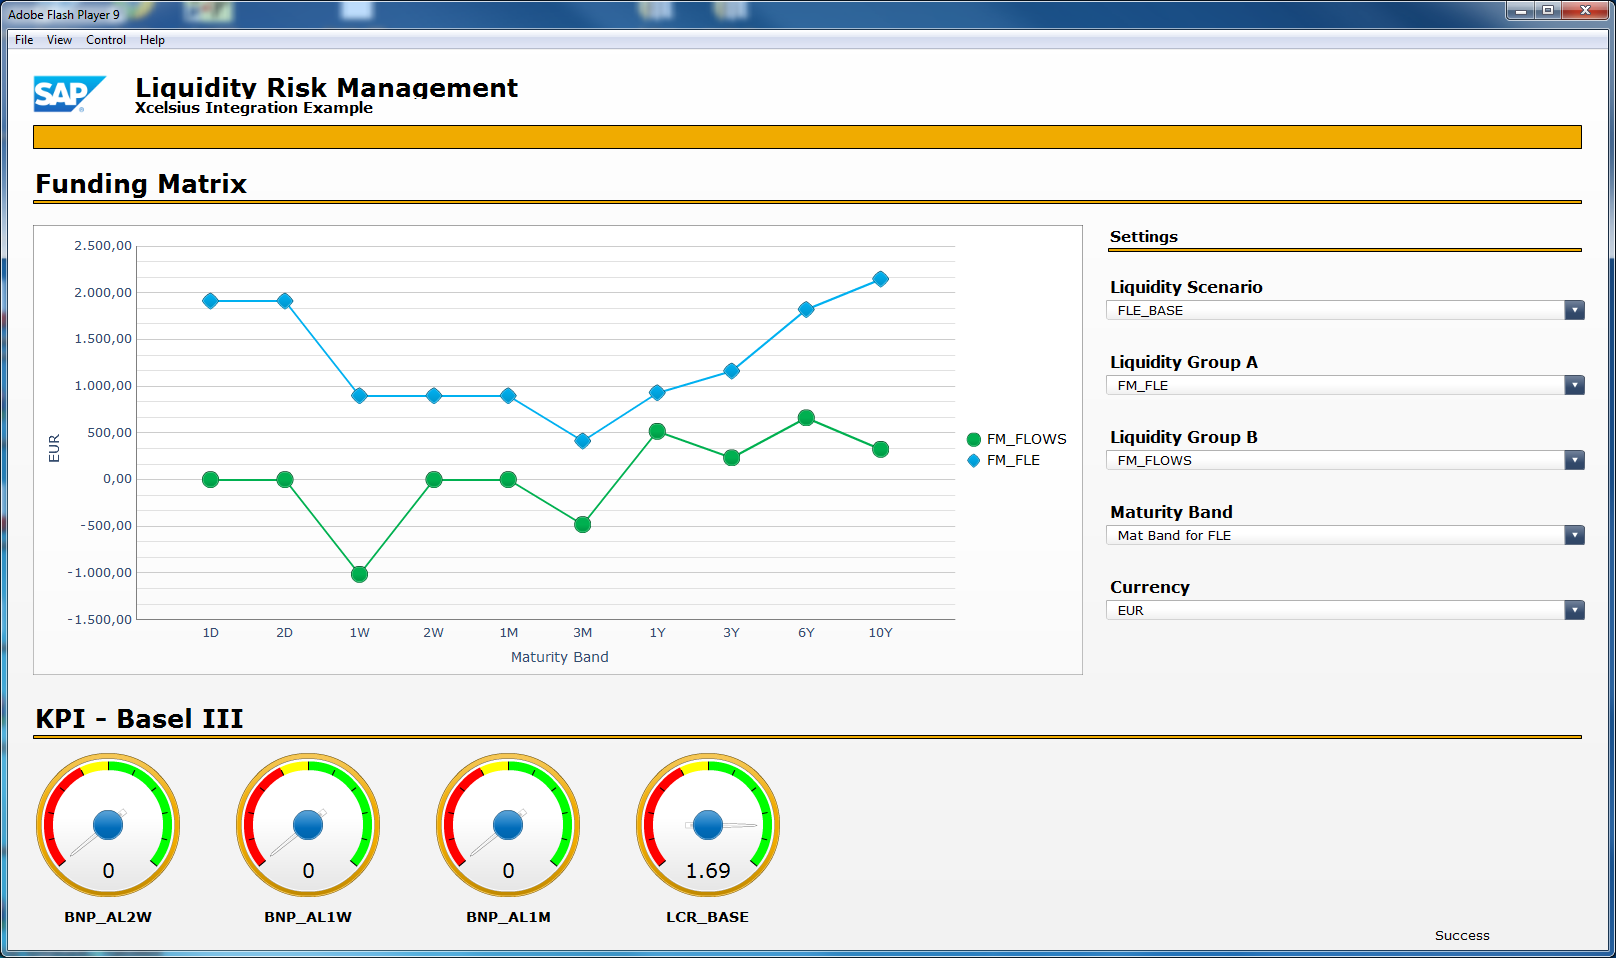
\includegraphics[width=15cm]{images/dashboard_preview.PNG}
\caption{BusinessObjects Xcelsius Dashboard mit den Daten des \gls{saplrm}\label{fig:umsetzung_dashboard}}
\end{figure} 

Es ist einfach zu erkennen, dass beide funktionalen Anforderungen mit der Erweiterung erfüllt werden können. Sowohl die Daten für die Kennzahlen, als auch die Daten für die Finanzierungsmatrix stehen zur Verfügung. In dem Beispiel ist eine Kennzahl mit dem Tachometer (unten) visualisiert, die Finanzierungsmatrix im oberen Teil als Liniendiagramm.

%\item[\anfl{uebertragbarkeit}] \textbf{Übertragbarkeit} \newline
%Im Rahmen der Bachelorarbeit wird exemplarisch die Anbindung einer weiteren Anwendung zur Auswertung an das \gls{saplrm} implementiert werden. Das Konzept der Umsetzung soll dennoch auf weitere Anwendungen übertragen werden können.
Die \anfRef{anf:uebertragbarkeit}{an die Übertragbarkeit } wird dadurch gewährleistet, dass die komplette Analyse programmiersprachenunabhängig durchgeführt wurde. Sie kann mit jeder objektorientierten Programmiersprache umgesetzt werden -- es müsste nur die Schnittstelle zu der eigentlichen Anwendung, also der Xcel\-si\-us\-Adap\-ter, entsprechend angepasst werden.


%\item[\anfl{erweiterbarkeit}] \textbf{Erweiterbarkeit} \newline
%Das \gls{saplrm} befindet sich aktuell noch in einer ersten Version in Entwicklung. Weitere Versionen sind schon jetzt in Planung. Zusätzliche Funktionen und Möglichkeiten, die in einer Weiterentwicklungen des \gls{saplrm} eingeführt werden, sollen mit möglichst geringem Aufwand auch auf die Erweiterung übertragen werden können.

%\item[\anfl{wartbarkeit}] \textbf{Wartbarkeit} \newline
%Um die Folgekosten der Erweiterung, zum Beispiel im Hinblick auf die Beseitigung von Fehlern, möglichst gering zu halten, soll eine gute Wartbarkeit von Anfang an bei der Entwicklung beachtet werden.
Durch den modularen Aufbau mit den verschiedenen ObjectProvidern können neue Funktionalitäten durch die Erstellung von weiteren Implementierungen leicht umgesetzt werden. Somit kann auch \anfRef{anf:erweiterbarkeit}{} als erfüllt betrachtet werden. Gleichzeitig wird dadurch die \anfRef{anf:wartbarkeit}{an die Wartbarkeit } abgedeckt.

%\item[\anfl{korrektheit}] \textbf{Korrektheit der Ergebnisse} \newline
%Die Daten, die mit Hilfe der Erweiterung in zusätzlichen Anwendungen verfügbar gemacht werden, müssen mit den Ergebnissen des \gls{saplrm} übereinstimmen. Nur wenn das sichergestellt ist, kann die Erweiterung sinnvoll genutzt werden.
Die Korrektheit der Ergebnisse, siehe \anfRef{anf:korrektheit}{}, wird dadurch sichergestellt, dass die Berechnungskomponente des \gls{saplrm} über die selbe Schnittstelle aufgerufen wird, wie es auch die Benutzeroberfläche in Oberon macht. Somit stimmen die Ergebnisse überein.

%\item[\anfl{sicherheit}] \textbf{Sicherheitsanforderungen} \newline
%Die Erweiterungen wird Zugang zu den Daten des \gls{saplrm} bieten. Es handelt sich dabei um vertrauliche Daten, die Zugangsbeschränkungen unterliegen. Es muss sichergestellt sein, dass die Zugangsbeschränkungen eingehalten werden und Daten nicht von unberechtigten Personen ausgelesen werden können.
Der Zugang zu den Daten ist, genau wie bei der existierenden iPad-Anwendung, durch Nutzer und Password vor unberechtigtem Zugriff geschützt. Dabei wird die gleiche Authentifizierungsmethode verwendet. Für potentielle Angreifer ist somit der Aufwand für unberechtigten Zugriff nicht geringer geworden -- \anfRef{anf:sicherheit}{} ist abgedeckt.

%\item[\anfl{leistung}] \textbf{Leistung} \newline
%Ein wichtiges Unterscheidungsmerkmal des \gls{saplrm} durch die Nutzung von \gls{HANA} ist die schnelle Analyse von Daten. Die Erweiterung soll die Geschwindigkeitsvorteile von \gls{HANA} auch in anderen Anwendungen verfügbar machen.
Schließlich bleibt noch \anfRef{anf:leistung}{}. Die Leistung aus der Sicht des Nutzers setzt sich aus der Zeit für die Berechnung der Werte durch die Berechnungskomponente und der eigentlichen Darstellung zusammen. Die Zeit für die Berechnung ist dabei festgesetzt und kann nicht beeinflusst werden. Die Zeit zur Darstellung ist dabei in \gls{xcelsius} mit der Erweiterung sogar schneller als die Darstellung mit dem Oberon Framework. Ein Hauptgrund ist hierbei das vergleichsweise langsame Rendern des Diagramms durch Oberon. Durch eine echt-parallele Verarbeitung der Webservice-Aufrufe könnte die Leistung der Erweiterung sogar noch gesteigert werden. Auch diese Anforderung ist somit erfüllt, obwohl sie bei der Entwicklung nicht im Mittelpunkt stand.

\section{Zusammenfassung}
In diesem Kapitel wurden die Evaluation der Erweiterung für \gls{xcelsius} durchgeführt. Diese hat ergeben, dass sich durch die reine Integration der Daten des \gls{saplrm} unter der bewussten Vermeidung von Vorgaben, was die Visualisierung oder die Art des Inputs und des Outputs betrifft, sich sehr viele Möglichkeiten ergeben. Es können alle Funktionen von \gls{xcelsius} genutzt werden, wodurch sich eine größere Flexibilität in der Auswertung der Daten des \gls{saplrm} bietet. Außerdem wurde die Abdeckung der gestellten Anforderungen überprüft und dabei festgestellt, dass die Anforderungen erfolgreich umgesetzt wurden.

\chapter{Zusammenfassung \& Ausblick}
% Fragestellung aus Einleitung aufgreifen \loreIpsum

Im Rahmen dieser Bachelorarbeit wurden zwei Ziele verfolgt. Auf der einen Seite sollte ein Konzept für die Nutzung weiterer Anwendungen in Verbindung mit der Berechnungskomponente des \gls{saplrm} entwickelt werden. Auf der anderen Seite sollte dieses Konzept für eine Anwendung beispielsweise umgesetzt werden. 

Das entwickelte Konzept basiert auf der Orchestrierung von Webservices. Dabei werden ein oder mehrere Webservices von der Zielanwendung konsumiert und die jeweiligen Ergebnisse orchestriert. Die Webservices nutzen dabei für den Bezug der Daten die Berechnungskomponente des \gls{saplrm}. Durch die Nutzung von weit verbreiteten Standards wie \gls{http} und \gls{xml} kann das Konzept einfach für verschiedene Anwendungen umgesetzt werden. Durch den modularen Aufbau, der durch die Orchestrierung der Webservices erreicht wird, ist auch eine gute Erweiterbarkeit sichergestellt. Durch eine Weiterentwicklung des \gls{saplrm} neu hinzugekommene Funktionen können einfach in das Konzept eingearbeitet werden. Außerdem wird durch den modularen Aufbau die spätere Wartung erleichtert.

Neben der Entwicklung des Konzeptes wurde im Rahmen der Bachelorarbeit die Umsetzung für \gls{xcelsius} durchgeführt. Das Ergebnis der Umsetzung ist eine Erweiterung, mit der die Einbindung von Daten, die auf der Berechnungskomponente basieren, erreicht werden kann. Durch die erfolgreiche Implementierung wurde gleichzeitig die Funktionsfähigkeit des Konzeptes gezeigt. Die Erweiterung wurde dabei so umgesetzt, dass die gewonnene Flexibilität von \gls{xcelsius} in vollem Umfang genutzt werden kann. Neben der bestehenden Oberfläche des \gls{saplrm} ist somit eine neue Möglichkeit zum Konsumieren der Daten hinzugekommen.

Mit der Erweiterung besteht erstmalig die Möglichkeit, das Liquiditätsrisikomanagement bei Banken in die Gesamtbankensteuerung einzubinden. Bestehende Dashboards von \gls{xcelsius} können mit Informationen über die Liquiditätssituation der Bank erweitert werden. Das erleichtert die Sicherstellung der Einhaltung von regulatorischen Vorschriften, wie zum Beispiel dem \gls{lcr} oder dem \gls{nsfr} im Rahmen von Basel III.

Basierend auf den Erkenntnissen dieser Arbeit bietet sich eine Umsetzung des Konzeptes für weitere Plattformen an. Eine Möglichkeit stellt dabei Panopticon, eine Anwendung zur Analyse von Echtzeitdaten, dar.\footnote{Panopticon -- http://www.panopticon.com/} Bezüglich der Anbindung von \gls{xcelsius} ist durch die dargestellte Sandbox-Limitierung und der daraus resultierenden Cross-Domain Request-Problematik Bedarf für Weiterentwicklungen gegeben. Weiterhin muss die Erweiterung stets an die Veränderungen durch die Weiterentwicklung des \gls{saplrm} angepasst werden.

Zusammengefasst lässt sich sagen, dass die Anbindung von weiteren Anwendungen viele neue Möglichkeiten für das Liquiditätsrisikomanagement bei Banken bietet. Die Implementierung für \gls{xcelsius} stellt eine lauffähige Version dar, bietet aber für die Zukunft noch Möglichkeiten für Weiterentwicklungen.

%	Ergebnisse der Arbeit wiedergeben

%	Arbeit in größeren Zusammenhang stellen

%	Ausblick auf mögliche Konsequenzen der Arbeit

%	Eigene Einschätzung








\end{onehalfspacing}


% -------------------------------------------------------------------------------------
% Anhang der Arbeit
% -------------------------------------------------------------------------------------
\seAppendix{}

\pagenumbering{Roman}
\setcounter{page}{8}


\chapter{Anhang}

\begin{lstlisting}[language=Java]
import java.io.*;
import java.net.*;
import javax.servlet.http.*;
import javax.servlet.*;
import sun.misc.BASE64Encoder;

@SuppressWarnings("serial")
public class ProxyServlet extends HttpServlet {

 public void doGet(HttpServletRequest req, 
  HttpServletResponse res) throws ServletException {
  try {
   String requestedUrl = req.getServletPath();
   String params = req.getQueryString();

   // build request url
   String urlString = "http://xhc.wdf.sap.corp"
    + requestedUrl;
   if (params != null)
    urlString += "?" + params;

   // build connection
   URL url = new URL(urlString);
   HttpURLConnection conn =
    (HttpURLConnection) url.openConnection();

   // set authorization
   BASE64Encoder encoder = new BASE64Encoder();
   String encoding = encoder.encode(
    "USER:PW".getBytes());
   conn.setRequestProperty("Authorization",
    "Basic " + encoding);

   // start request
   conn.setRequestMethod("GET");
   conn.connect();

   PrintWriter out = res.getWriter();
   BufferedReader reader = new BufferedReader(
   new InputStreamReader(
    conn.getInputStream()));

   // get response
   String content = null;
   while ((content = reader.readLine()) != null) {
    out.print(content);
   }

   out.flush();
   out.close();
  } catch (Exception e) {
   System.err.println("Request failed");
  }  
 }
\end{lstlisting}

\begin{programm}[ht]
\begin{lstlisting}
}
\end{lstlisting}
\caption{Proxy-Servlet zur Umgehung der Cross-Domain Request Beschränkungen\label{listing:servlet}}
\end{programm}

%\caption{Proxy-Servlet zur Umgehung der Cross-Domain-Request Beschränkungen\label{listing:servlet}}
%\end{programm}


% -------------------------------------------------------------------------------------
%  Erzeugung eines Glossars
% -------------------------------------------------------------------------------------
\newpage
\sePrintGlossary{}

% -------------------------------------------------------------------------------------
% Literaturverzeichnisses
% -------------------------------------------------------------------------------------
\sePrintBibliography{}


% Sammelwerke, die in der Grundform vorkommen sollten!
%\nocite{Bar.08}
%\nocite{Rom.10}
%\nocite{Zer.10}
%\nocite{Hof.11}
%\nocite{Eve.08}

\bibliographystyle{sty/bibliothek-style}
\seBibliography{literatur}

% -------------------------------------------------------------------------------------
% Erzeugung der ehrenw\"ortlichen Erkl\"arung
% -------------------------------------------------------------------------------------
\seEhrenwoertlicheErklaerung{}

\end{document}
